\documentclass[11pt]{article}

% ---------- Page geometry ----------
\usepackage[margin=1in]{geometry}
\usepackage[utf8]{inputenc}
\usepackage[T1]{fontenc}
\usepackage{lmodern}
\usepackage{microtype}
\usepackage{setspace}
\onehalfspacing
\emergencystretch=3em

% ---------- Math / symbols ----------
\usepackage{amsmath,amssymb}

% ---------- Graphics / tables ----------
\usepackage{graphicx}
\usepackage{booktabs}
\usepackage{longtable}
\usepackage{array}
\usepackage{multirow}
\usepackage{caption}
\captionsetup{font=small, labelfont=bf}
\usepackage{float}
\usepackage{adjustbox}
\usepackage{xcolor}
\usepackage[strings]{underscore}

% ---------- Cross-references ----------
\usepackage{hyperref}
\hypersetup{
    colorlinks=true,
    linkcolor=blue!50!black,
    citecolor=blue!40!black,
    urlcolor=blue!50!black,
    pdftitle={From Institutional Emergence to Historically Structured Continuity},
    pdfauthor={Kan Yuenyong}
}
\usepackage[capitalize,noabbrev]{cleveref}

% ---------- Bibliography ----------
\usepackage[backend=biber, style=authoryear, maxcitenames=2, maxbibnames=99, doi=false, isbn=false, url=true]{biblatex}
\addbibresource{references.bib}

% ---------- Section numbering depth ----------
\setcounter{secnumdepth}{3}
\setcounter{tocdepth}{2}

% ---------- Title ----------
\title{\textbf{From Institutional Emergence to Historically Structured Continuity:\\
An Outcome-Blind Agent-Based Search for Recurrent Governance Forms}}
\author{Kan Yuenyong}
\date{\today}

\begin{document}

\maketitle

\begin{abstract}
A companion dissertation uses structural equation modeling (SEM) on World
Values Survey data to identify a two-dimensional latent governance space
--- State Capacity ($S$) and Institutional Constraint ($Z$) --- and, within
it, three qualitatively theorized regions of empirically observed
governance configurations. The dissertation's own text is explicit that
this SEM result defines a coordinate space rather than classifying
countries into discrete types, and explicitly calls for future clustering
work to test whether those regions are, in fact, statistically discrete.
We report a four-stage, outcome-blind agent-based search for recurrent
institutional phenotypes that takes that open question seriously as a
generative one: can heterogeneous governance configurations, and
historically structured movement between them, emerge endogenously from
atomic microscopic mechanisms alone, with no governance typology, trajectory
count, or macro-level target ever encoded as a rule or a selection
criterion? Level 1.2 (24-run open discovery) and Level 1.2b (an ecologically
stratified, ledger-audited, 576-run rediscovery with an independent
384-run confirmation pool) establish that the tested synchronic substrate
is generatively sufficient --- it produces institutions and heterogeneous
institutional outcomes from purely local rules --- but not, by itself,
sufficient to compress those outcomes into a small number of discrete,
recurring forms: both milestones return a \texttt{continuum} verdict,
independently replicated on fresh data. Level 1.3 and Level 1.3b extend the
model with a historical operator, $M_{\text{historical}} = M_{\text{general}}
+ H$, formalizing $H$ as three wired pressure-transmission channels
(security, bargaining, coordination-complexity pressure), institutional
entrenchment, and dual performance/procedural legitimacy ledgers, and ask
whether history, as such, causally and persistently shapes institutional
trajectories even where it does not resolve them into discrete families.
It does. A sham-validated (12/12 byte-identical control match), matched-seed
causal intervention design finds that erasing, reversing, or exposure-
equalizing a run's realized pressure history produces a real, non-decaying,
in several tests \textit{growing} divergence from that same run with its
own history intact (final-sustained $|S_{\text{obs}}|$ gaps of
0.054--0.072); pressure-onset ordering produces a real but modest and
direction-inconsistent effect (24.1\%/32.4\% of 108 matched contrasts
statistically distinguishable on $S_{\text{obs}}$/$Z_{\text{obs}}$); and an
observer-side $S_{\text{obs}}$--$Z_{\text{obs}}$ coupling, real but modest
and sensitive to measurement weighting (Pearson $r\approx0.26$--$0.29$
across defensible variants, roughly halving to $r\approx0.14$ under an
equally defensible alternative), corroborates rather than reproduces the
dissertation's own $S$/$Z$ axes without being the same construct. A
formal eight-way decision-gate classification, reusing Level 1.2b's own
frozen discreteness rule unmodified, again returns \texttt{persistent\_%
continuum}: an eight-component Gaussian mixture achieves the lowest Bayesian
information criterion among tested candidates, but no $k$ from 1 to 8
clears even a 0.15 silhouette floor, cross-algorithm agreement is weak once
non-independent fits are excluded (adjusted Rand index 0.016--0.357), and
the partition does not reproduce across ecological strata (adjusted Rand
index $-0.043$ to $-0.014$) --- a statistical-component count is not, and
must not be read as, a count of institutional species. We conclude that
history is a real, causally demonstrated, persistent conditioning operator
on where a governance configuration sits and how it got there, without
collapsing the underlying space into the three, or any small fixed number
of, discrete attractors; the dissertation's three empirically observed
trajectories remain a legitimate empirical finding at their own analytical
level, best read as historically and institutionally interpreted regions of
a continuous, path-dependent configuration space that this model's own
generative and historical mechanisms are jointly sufficient, but not yet
calibrated, to explain in full.

\end{abstract}

\clearpage
\tableofcontents
\clearpage

\section{Introduction}
\label{sec:introduction}

A companion dissertation, \textit{Positive Governance}
\parencite{yuenyong2025positive}, uses structural equation modeling (SEM)
on World Values Survey data to identify a two-dimensional latent governance
space --- a State Capacity factor ($S$) and an Institutional Constraint
factor ($Z$, combining rule of law and democratic accountability) --- and
argues that this space, not a single one-dimensional governance ranking
such as the World Bank's Worldwide Governance Indicators, is the right unit
for comparative analysis. Within that space, the dissertation identifies
three qualitatively \textit{theorized} regions of empirically observed
governance configurations, which it labels Authoritarian Efficiency,
Constrained Liberalism, and Integrated Equilibrium. It is important, and a
central methodological commitment of this paper, to state precisely what
the dissertation itself claims for these three regions and what it does
not. The dissertation's own text is explicit that SEM ``does not classify
countries or predict trajectories; it defines the coordinate space,'' and
its own concluding chapter calls explicitly for \textit{future} work using
``unsupervised learning methods (e.g., cluster analysis, t-SNE) to
empirically identify governance archetypes.'' No clustering algorithm was
run on the SEM output to derive three trajectories; three is a qualitative,
interpretive typology laid over a statistically identified two-dimensional
space, not a statistically discovered partition count. We take this
distinction seriously throughout, because it is exactly the empirical
question a generative, agent-based search can speak to in a way a
cross-sectional SEM cannot: whether heterogeneous governance configurations,
and structured movement between them, can emerge \textit{endogenously} from
elementary micro-level mechanisms, with no typology, count, or macro-target
ever built in.

This paper reports a four-stage program of outcome-blind agent-based
search, structured around the dissertation's own governing equation,
$G = f(S, Z)$, extended by an unoperationalized external-influence term
$\beta$ the dissertation itself leaves open. We ask a bottom-up question the
dissertation's top-down SEM analysis cannot: if a population of
heterogeneous agents is given only elementary relational, ecological, and
organizational mechanisms --- cooperation, punishment, imitation, exit, a
resource ecology with real material accounting, proto-institutional rule
formation, delegation, monitoring, accountability, mobility, and
interpatch coordination --- and no encoding whatsoever of $S$, $Z$, or any
trajectory label, what persistent macroscopic governance patterns, if any,
emerge from the resulting dynamics, and does adding historically structured
pressure, sequencing, and entrenchment change the answer?

\subsection{From a synchronic null to a historically conditioned question}
\label{sec:intro-synchronic-to-historical}

The paper's first two milestones, Level 1.2 and Level 1.2b (in this
project's own internal numbering, continuing from an earlier development
sequence summarized in \cref{sec:model-genealogy}), tested a
\textit{synchronic} substrate: every simulated jurisdiction faces
materially the same menu of possible institutional configurations at
materially the same starting conditions, differing only in randomly drawn
traits and parameter draws, with no historically asymmetric pressure,
sequencing, or path-dependent lock-in represented anywhere. That search,
conducted twice --- once at a modest scale legitimately confounded by
near-universal ecological collapse, and once at roughly 24 times the scale
with that confound explicitly removed through exact ecological accounting
and ex-ante feasibility stratification --- did not independently recover a
small number of discrete, well-separated institutional forms. Both
milestones returned a \texttt{continuum} verdict, independently replicated
on fresh, disjoint data. We reported this as a positive, informative
finding, not a shortfall: the tested atomic governance ecology is
\textit{generatively sufficient} to produce institutions and heterogeneous
institutional outcomes from purely local rules, while showing, with real
statistical force, that generative sufficiency does not by itself imply
convergence onto a small number of recurring forms. We closed that
milestone by proposing, as the natural next hypothesis rather than a
finding already in hand, a formal decomposition

\begin{equation}
M_{\text{historical}} = M_{\text{general}} + H
\label{eq:historical-decomposition-intro}
\end{equation}

where $M_{\text{general}}$ is the synchronic substrate Level 1.2/1.2b
tested and $H$ denotes historically structured pressures, sequencing, and
entrenchment --- explicitly not implemented or tested at that time.

Level 1.3 and Level 1.3b, reported here for the first time, implement and
test $H$. They wire three pressure-transmission channels (security
pressure, bargaining pressure, and coordination-complexity pressure, each
via two of six candidate transmission mechanisms), institutional
entrenchment (age-dependent resistance to change), and dual
performance/procedural legitimacy ledgers into the same generative
substrate Level 1.2/1.2b already validated, and ask, generatively and then
causally, whether historically structured pressure and sequencing move the
institutional outcome space in ways a synchronic substrate cannot. Because
the observer layer's own $S$ and $Z$ composites ($S_{\text{obs}}$,
$Z_{\text{obs}}$; \cref{sec:observer-metrics-l13}) are constructed
independently of, and are not the same object as, the dissertation's SEM
latent factors, this program provides three complementary, non-duplicative
kinds of evidence about the dissertation's own $S$/$Z$ framework: whether a
generative mechanism set can produce heterogeneous configurations
distributed along axes that plausibly correspond to state capacity and
institutional constraint; whether a real, causal, historically structured
process shapes movement through that space; and whether the resulting
structure is discrete, in the way a three-trajectory typology would
require, or continuous.

\subsection{What this paper establishes, in sequence}
\label{sec:intro-sequence}

Six things are established across the paper's four linked milestones:

\begin{enumerate}
\item A general microscopic governance-generative agent-based model (ABM)
  was constructed, built strictly from agent-level mechanisms addressing
  cooperation, ecological viability, information, enforcement, delegation,
  accountability, mobility, and interpatch coordination
  (\cref{sec:model-methods}), with a structural firewall mechanically
  preventing any dissertation vocabulary, symbol, or trajectory label from
  ever entering the generative or observer layers.
\item An outcome-blind statistical search at Level 1.2/1.2b did not
  independently recover three discrete institutional types, or any small,
  stable number of them, in the synchronic substrate
  (\cref{sec:level12,sec:level12b}); both the initial and the ecologically
  stratified, 24-times-larger rediscovery returned an independently
  replicated \texttt{continuum} verdict.
\item Level 1.3 extended the substrate with historically structured
  pressure, sequencing, and entrenchment mechanisms and found, on pooled
  observational data, real ordering-dependent variation, a real
  (if construction-audited) $S_{\text{obs}}$--$Z_{\text{obs}}$ coupling, and
  a headline discovery result that itself failed independent fresh-data
  reproduction --- evidence leaning \texttt{continuum} again, but on a
  pooled, not purpose-designed, evidentiary base (\cref{sec:level13}).
\item Level 1.3b validated Level 1.3's findings with a purpose-designed,
  preregistered, eight-hypothesis program including, for the first time in
  this project, a sham-controlled causal intervention stage: erasing,
  reversing, or exposure-equalizing a run's realized pressure history
  produces real, persistent, non-decaying divergence from that run's own
  intact history, validated against a byte-identical sham control that
  itself introduces zero spurious divergence (\cref{sec:level13b}). History,
  in this precise causal sense, matters.
\item That same purpose-designed program, applying Level 1.2b's own frozen
  discreteness classifier unmodified, found the historically extended
  substrate's outcome space to be, if anything, \textit{more} decisively
  continuous than the synchronic substrate was: no tested $k$ from 1 to 8
  clears even the classifier's entry-level silhouette floor, cross-algorithm
  agreement is weak, and the leading eight-component partition does not
  reproduce across ecological strata (\cref{sec:level13b,sec:results}).
\item Taken together, the four milestones support a specific, bounded
  claim, stated precisely and repeatedly to avoid the very overclaiming this
  paper's own terminological discipline (\cref{sec:terminology-discipline}) is
  built to prevent: the governance space this model generates is
  historically structured, heterogeneous, and continuous --- not
  historically inert, and not discretely speciated into three, eight, or
  any other fixed count of institutional forms, using the precise
  vocabulary fixed in \cref{sec:terminology-discipline}
  (\cref{sec:discussion,sec:conclusion}).
\end{enumerate}

\subsection{Methodological triangulation, not duplication}
\label{sec:intro-triangulation}

We are explicit throughout that this paper's ABM evidence and the
dissertation's SEM evidence answer different questions at different
analytical levels, and that neither substitutes for the other.
\Cref{sec:disc-triangulation} develops this in full; in outline, the SEM
analysis \textit{identifies} a two-dimensional coordinate space from
cross-sectional survey data on real, already-formed states at one
historical moment; the ABM's generative layer establishes whether a
microscopic mechanism set is \textit{sufficient} to produce heterogeneous
configurations occupying an analogous space from nothing; and the ABM's
historical layer, uniquely, supports controlled causal experimentation ---
erasing or reversing a specific run's own history and comparing it against
itself, sham-validated --- that cross-sectional survey data structurally
cannot support at all. These three lines of evidence triangulate toward a
single account without duplicating each other, and no single one of them,
including this paper's own simulation results, is sufficient on its own to
settle whether real governance systems are, in fact, discretely speciated;
that stronger claim would require historically calibrated data this paper
does not use (\cref{sec:limitations}).

\subsection{Roadmap}
\label{sec:intro-roadmap}

Section~\ref{sec:theoretical-motivation} situates the project relative to
agent-based computational social science, common-pool-resource governance,
historical institutionalism and path dependence, and the methodological
literature on null results and discreteness testing in clustering.
Section~\ref{sec:model-genealogy} summarizes the level-by-level development
sequence, including Level 1.3/1.3b's own place in it.
Section~\ref{sec:model-methods} documents the full model and discovery
methodology, including the historical pressure/entrenchment/legitimacy
machinery and the extended eight-way decision-gate vocabulary.
Sections~\ref{sec:level12} and~\ref{sec:level12b} report the synchronic
Level 1.2/1.2b program; Sections~\ref{sec:level13}
and~\ref{sec:level13b} report the historical Level 1.3/1.3b program.
Section~\ref{sec:results} consolidates every headline quantitative result
across all four milestones. Section~\ref{sec:discussion} develops the
paper's theoretical synthesis: the richer generative state
$\mathcal{G}_t = [S_t, Z_t, H_t, E_t, L_t, P_t, R_t, C_t, \ldots]$, the
triangulation logic linking SEM identification, ABM generative sufficiency,
and historical causal experimentation, and a precise, bounded reading of
the relationship to the dissertation's own three trajectories.
Sections~\ref{sec:limitations}--\ref{sec:reproducibility} close with
limitations, conclusions, and reproducibility information. Appendices
provide a compact ODD-style model summary extended for Level 1.3/1.3b, full
parameter and outcome-count tables, the recurrence and decision-gate
procedures, the ledger accounting identities, and a condensed evidence
ledger mapping every numerical claim in this paper to its source file and
field; the complete claim-by-claim manifest is maintained separately in
\texttt{claim\_evidence\_manifest.csv}.

\section{Theoretical Motivation}
\label{sec:theoretical-motivation}

\subsection{Governance as an emergent relational ecology}
\label{sec:emergent-ecology}

Agent-based computational social science treats macro-level social pattern
as an emergent consequence of micro-level rules, rather than as a
directly-specified target
\parencite{epstein1996growing,railsback2019agent}. The tradition most
directly relevant here descends from two distinct lines: iterated-game
accounts of cooperation, reciprocity, and costly punishment
\parencite{axelrod1984evolution,axelrod1981evolution,fehr2002altruistic},
and empirically grounded common-pool-resource governance research
\parencite{ostrom1990governing,janssen2006empirically,poteete2010working}.
Ostrom's fieldwork identified design principles --- clearly defined
boundaries, congruence between rules and local conditions, collective-choice
arrangements, monitoring, graduated sanctions, conflict-resolution
mechanisms, and nested enterprises --- under which self-governing
institutions for shared resources persist without either central
authority or privatization. Our model does not encode these principles
directly; it encodes the more elementary primitives (extraction,
maintenance, monitoring, sanctioning, delegation, coordination) from which
such principles, if they matter, would have to emerge as statistical
regularities in simulated outcomes, not as assumed structure.

\subsection{From atomic interactions to proto-institutions}
\label{sec:atomic-to-proto}

The project's own development sequence (\cref{sec:model-genealogy}) is
built explicitly bottom-up: a population of heterogeneous agents interacts
bilaterally under a repeated cooperation/defection grammar with imperfect
observation, memory, and optional costly punishment; the population is
coupled to a materially accounted resource ecology; and only once that
ecology's own dynamics were understood did the project introduce a
locally shared, voluntarily adopted, imperfectly monitored and enforced
rule --- a \textit{proto-institution} --- as an opt-in generative
mechanism. Proto-institutions are then extended with delegation
(administrative capacity accumulated from realized performance, never
granted as a trait), discretion and its accountability counterweight
(audit, appeal, recall), and interpatch coordination. At every stage, the
mechanism defaults to a verified, byte-for-byte no-op, so that each new
layer is additive rather than a silent redefinition of what came before.

\subsection{Recurrent institutional phenotypes versus imposed typologies}
\label{sec:recurrent-vs-imposed}

A central methodological commitment of this project, enforced structurally
rather than merely stated, is that the generative layer never encodes a
governance typology, and the observer layer never imposes one on the
results before the results are seen. We use \textit{recurrent
institutional phenotype} throughout, rather than \textit{institutional
type} or \textit{governance regime}, to mark this distinction: a phenotype
is a statistically discovered pattern in an observer-computed feature
vector, evaluated against explicit stability and recurrence criteria; it is
never a category the model was built to produce. This distinguishes our
approach from ABM applications that calibrate agent rules to reproduce a
known macro-target. Here the target category count is itself an open
empirical question the discovery pipeline is asked, not told.

\subsection{Historical institutionalism, path dependence, and critical junctures}
\label{sec:historical-institutionalism}

A separate literature, largely orthogonal to the agent-based tradition
above, argues that governance outcomes are shaped not only by
contemporaneous structural conditions but by the specific historical
sequence through which institutions formed: critical junctures at which
a range of outcomes was genuinely possible, followed by increasing-returns
dynamics that make an early institutional choice progressively more costly
to reverse \parencite{pierson2000increasing,mahoney2000path,capoccia2007critical};
the long shadow of colonial extraction versus
settlement patterns and early state-building choices on later institutional
quality \parencite{acemoglu2012why,northwallisweingast2009}; and the
broader claim that political order and its erosion are themselves
historically contingent processes, not fixed endpoints
\parencite{fukuyama2014political,north1990institutions}. This literature
supplies the theoretical vocabulary --- sequencing, entrenchment, critical
juncture, lock-in --- that Level 1.3/1.3b's own historical mechanisms
operationalize generatively (\cref{sec:level13}); it does not, by itself,
adjudicate whether path-dependent processes compress governance outcomes
into a small number of discrete, recurring configurations or instead
produce a continuously varying space with graded, historically contingent
structure. That is an empirical question this paper's own historical
discovery program is built to ask without presupposing the answer, in the
same outcome-blind spirit as Level 1.2/1.2b's synchronic search.

The dissertation's own governance-indicator critique is relevant here too.
Aggregate governance rankings such as the World Bank's Worldwide Governance
Indicators \parencite{kaufmann2011worldwide} compress multiple correlated
component indicators onto a single latent dimension via an unobserved
components model, an approach the dissertation argues collapses
theoretically distinct dimensions --- capacity to act and constraint on
how that capacity may be used --- into one ranking, and which is, by
construction, silent on historical trajectory: a single cross-sectional
score cannot represent how a state arrived at its current position, only
where it currently sits. The dissertation's own two-dimensional $S$/$Z$
reframing is explicitly a response to this limitation; this paper's own
historical extension is a further response, adding a third
axis --- historical trajectory itself --- that neither a one-dimensional
ranking nor a two-dimensional cross-sectional coordinate space can
represent.

\subsection{Terminological discipline}
\label{sec:terminology-discipline}

This paper uses five terms that name related but analytically distinct
objects, and treats confusing them as a substantive error rather than a
stylistic one, given how directly this project's own headline findings turn
on the distinction. A \textit{configuration} is a specific, realized point
in the observer-computed feature space (Level 1.2/1.2b's ten-dimensional
phenotype vector, or Level 1.3/1.3b's fourteen-dimensional extension) ---
one simulated jurisdiction's own outcome, nothing more. A
\textit{statistical component} is a fitted element of a clustering or
mixture model (a Gaussian-mixture component, a hierarchical-clustering
branch) --- a property of a fitting procedure applied to a finite sample,
not by itself evidence of anything in the underlying process. A
\textit{recurrent institutional phenotype} is a statistical component that
has additionally cleared this project's own preregistered recurrence
criteria (\cref{sec:discovery-procedure}) --- cross-seed recurrence,
cross-algorithm support, bootstrap stability, and the rest --- evaluated
by strict conjunction, never a majority. A \textit{dynamical attractor} is
a further, stronger claim this project has never made about any discovered
structure: that a system returns to a specific state after perturbation,
which requires direct, disclosed evidence of majority recovery on every
tracked dimension (\cref{sec:level12b-scale-causal}), not merely that a
state persists once reached. An \textit{empirical trajectory}, finally, is
the dissertation's own object: a qualitatively interpreted region of its
SEM-identified $S$/$Z$ space, populated by real countries' survey-measured
positions, which this paper's own simulation results can inform but cannot
directly confirm or refute (\cref{sec:disc-relationship-to-dissertation}).

We use \textit{historically structured, heterogeneous governance
continuum} as this paper's own preferred summary phrase for what Level
1.3/1.3b's evidence supports, and, where the evidence licenses a
marginally stronger reading, \textit{a continuous institutional space
containing conditional path dependence and possible metastable regions}
--- never stronger than that. We do not, anywhere in this paper, claim that
the model discovered exactly three or exactly eight governance species,
that the ABM's own discovery pipeline found three attractors corresponding
to the dissertation's trajectories, that path dependence in this model is
universal or historically deterministic, or that any simulation result in
this paper empirically validates the dissertation's own trajectory
typology. Each of these five specific claims is one this paper's own
evidence does not support, and \cref{sec:disc-boundary-claims} states
explicitly, alongside the positive findings, why each is ruled out.

\subsection{Why null discovery is theoretically informative}
\label{sec:why-null-informative}

A discovery procedure that always finds structure is not informative about
whether structure exists; it is informative only about the procedure's own
bias. The clustering-methodology literature treats this directly: cluster
stability under resampling and under alternative algorithms is itself the
primary evidence for whether a partition reflects real structure or
artifact of the fitting procedure
\parencite{benhur2002stability,vonluxburg2010clustering,hubert1985comparing,rousseeuw1987silhouettes}.
Model-based (finite-mixture) clustering in particular is well known to
overfit at modest sample sizes, producing spuriously confident partitions
that do not generalize to held-out data \parencite{fraley2002model};
density-based clustering supplies a structurally different failure mode
(explicit noise, no forced full-coverage partition) precisely so that a
finding of "structure" is not an artifact of a single clustering
family's own inductive bias \parencite{campello2013density}. Reporting a
well-designed null result --- one that would have detected recurrent
structure had it been there, evaluated by multiple algorithms and
independently replicated on fresh data --- is therefore not merely
permissible negative-results hygiene; in a discovery setting it is direct,
positive evidence about the shape of the underlying outcome space. This is
the logic \cref{sec:level12,sec:level12b} apply throughout: every reported
null is a preregistered, multiply-corroborated, independently replicated
finding, not an absence of search.

\section{Model Genealogy}
\label{sec:model-genealogy}

Level 1.2 and Level 1.2b are not a single design decision; they sit at the
end of an eight-milestone development sequence in which each mechanism was
introduced, defaulted to an exact no-op, and validated before the next
layer was added. Level 1.3 and Level 1.3b, the historical extension this
paper's second half reports, continue that same discipline directly:
every historical mechanism they add --- pressure-transmission channels,
entrenchment, dual legitimacy ledgers --- was itself introduced, defaulted
to a verified no-op, and mechanism-validated before any discovery or causal
experiment consumed it. This section summarizes the full ten-milestone
sequence to make clear what was already established, and under what
conditions, before each discovery pipeline reported later in this paper was
ever run. Full detail for every milestone below is in the source
repository's own per-level scientific notes and ODD addenda (see
\cref{sec:reproducibility}); this section reports only what is load-bearing
for interpreting the results that follow.

\begin{table}[htbp]
\centering
\caption{Model layers and mechanisms by milestone. Every mechanism
defaults to a verified, byte-for-byte no-op unless explicitly activated.}
\label{tab:mechanism-layer}
\adjustbox{max width=\textwidth}{\begin{tabular}{@{}lll@{}}
\toprule
\textbf{Milestone} & \textbf{Layer / mechanism added} & \textbf{Default state} \\
\midrule
Level 0 / 0.1 & Bilateral cooperation/defection, punishment, imitation, exit; resource pool & always active \\
Level 0.2     & Viability state machine, fitness modes, participation accounting & no-op (\texttt{viability\_mode="none"}) \\
Level 0.3 / 0.3b & Independent ecological policy; local patches; audited regime classifier & no-op (\texttt{ecology\_topology="global\_pool"}) \\
Level 1.0     & Proto-institution: propose/adopt/monitor/sanction/amend/dissolve & no-op (\texttt{rule\_formation\_enabled=False}) \\
Level 1.1     & Delegation, capacity, discretion, accountability, contributions, coordination & no-op (\texttt{delegation\_enabled=False}, etc.) \\
Level 1.1b    & Mechanism-substream RNG; audited delegation classifier & no-op (\texttt{rng\_mode="legacy\_single\_stream"}) \\
Level 1.2     & Local observation, transmission, migration, scaling; phenotype vector \& blind discovery & no-op (5 mechanism flags default off) \\
Level 1.2b    & Ecological ledger, feasibility ratios, feature/recurrence audits, stratified rediscovery & no new fields; reuses \texttt{level12\_complete} \\
Level 1.3     & Pressure-transmission channels (security/bargaining/coordination), entrenchment, dual legitimacy ledgers, $S_{\text{obs}}$/$Z_{\text{obs}}$ composites & no-op (channel flags default off) \\
Level 1.3b    & Sham-controlled history-erasure intervention, purpose-designed discovery/confirmation, measurement-weighting audit & no new fields; validation milestone only \\
\bottomrule
\end{tabular}
}
\end{table}

\subsection{Level 0: atomic relational mechanisms}
\label{sec:level0}

The base model (Level 0 and its Level~0.1 ecological-closure extension) is
a heterogeneous population interacting over a dynamic network via a
repeated cooperation/defection payoff grammar, with imperfect observation,
memory and forgiveness, optional costly punishment, strategy imitation
with low-rate mutation, and costly relationship exit and formation. Level
0.1 closes the resource loop with a shared, bounded environment pool
governed by logistic regeneration and mandatory subsistence costs, and
makes relationship dynamics genuinely ongoing rather than an
initialization-time artifact. Every stochastic draw in the codebase passes
through one explicit, seeded random-number generator, making every run
exactly reproducible from its configuration.

\subsection{Ecological closure and viability}
\label{sec:ecological-closure}

Level 0.2 added full participation-opportunity accounting, a disableable
agent viability state machine (distress, dormancy, and, only if
explicitly enabled, removal and replacement), configurable imitation
fitness signals, explicit ecological supply/demand balance accounting, and
operational (never "attractor"-labeled) dynamical classification
definitions. This milestone's own investigation into Level 0.1's pool
collapse and near-universal measured cooperation found both candidate
explanations it tested --- selective-participation bias and
relative-fitness invariance to universal impoverishment --- genuinely
present, with regime-dependent relative weight.

\subsection{Endogenous ecological behavior}
\label{sec:endogenous-ecology}

Level 0.3 gave agents a second, structurally independent behavioral
dimension --- an ecological action (extraction, maintenance, or restraint)
governed by its own policy, never derived from the social
cooperate/defect decision --- and an opt-in spatially disaggregated
alternative to the single global pool: fixed-membership local patches.
Four causal-intervention counterfactuals (no environmental effect, and
frozen, randomized, or shuffled ecological policy) were built so that any
observed persistence could be attributed to actual agent behavior, not
merely to the bare environmental equation. Level 0.3b then re-audited Level
0.3's own regime classifier with a stricter, burn-in-aware, multi-criterion
test and a prospectively registered confirmation pipeline; the audited
classifier found none of the original "oscillatory" or "intermittent"
labels survived across 144 point-seed runs, and established, via a
paired, prespecified causal comparison, that endogenous adaptive
ecological behavior causally worsens ecological persistence relative to
frozen or randomized counterfactuals. This causal result --- not a
discretionary preference --- was the two-route decision gate that licensed
proceeding to institutional mechanisms at all.

\subsection{Proto-institutions, delegation, accountability, and coordination}
\label{sec:proto-institutions}

Level 1.0 introduced the proto-institution substrate directly in response
to Level 0.3b's demonstrated coordination failure: a locally shared,
patch-attached rule that can be proposed, voluntarily adopted, imperfectly
monitored and enforced, amended, dissolved, and --- possibly ---
reconstructed, entirely from local information. Level 1.0's own
counterfactual comparison found persistent proto-institutions emerged
unforced at every tested ecological candidate, alongside a
directionally consistent (not, at that milestone's sample size,
statistically confirmed) pattern in which real monitoring and
sanctioning infrastructure was associated with \textit{lower} final
ecological occupancy than no institution at all. Level 1.1 then built the
generative bridge from a single static rule to delegation: administrative
capacity accumulated only from realized task performance (never a static
trait), discretion and its corresponding appropriation opportunity,
accountability (audit, recall, appeal), opt-in collective contributions,
and minimal bilateral interpatch coordination, deliberately independent of
delegation. Level 1.1b then validated these mechanisms directly ---
artifact-independent re-verification, a per-mechanism random-number
substream architecture for causal ablations, and an audited, more
conservative delegation classifier reported alongside the original for
direct comparison, never replacing it.

\subsection{Why Level 1.2 was the appropriate discovery gate}
\label{sec:why-level12}

Only once local institutional formation, delegation, accountability, and
coordination were each independently built, defaulted to exact no-ops, and
mechanism-validated in isolation did the project introduce the mechanisms
that make institutions capable of \textit{propagating and competing for
persistence across space} --- local observation, component-wise
transmission, migration and membership selection, differential
persistence, and institutional scaling --- and, simultaneously, the
observer-only apparatus needed to ask, without bias toward any answer,
whether recurrent institutional configurations exist at all: a
ten-dimensional phenotype vector, temporal feature extraction, a blind
discovery pipeline, and a twelve-criterion recurrence test. This is Level
1.2. Running an outcome-blind discovery search before this point would have
been premature (institutions could not yet propagate or compete); running
it very much later, without first establishing that every prior mechanism
defaults to a verified no-op and is individually validated, would have
made any discovered (or undiscovered) structure impossible to attribute to
specific, understood mechanisms. Level 1.2 is where those two
requirements are jointly first satisfied.

\subsection{Why Level 1.3 was the appropriate historical-extension gate}
\label{sec:why-level13}

Level 1.2b's own closing synthesis (\cref{sec:level12b-verdict}) established
that the synchronic substrate is generatively sufficient but not
phenotype-convergent, and explicitly motivated, without implementing or
testing, a historically conditioned extension
(\cref{eq:historical-decomposition-intro}). Only once that synchronic
result was independently replicated on fresh data, and only once the
project's own ecological ledger, feasibility measures, and recurrence
machinery were validated at the 576-run scale, did the project introduce
history as a generative mechanism: three pressure-transmission channels
(security, bargaining, coordination-complexity), each wired through two of
six candidate transmission primitives shared across channels
(\texttt{pressure\_adjusted\_probability}, \texttt{pressure\_adjusted\_%
scale}); institutional entrenchment (age-dependent resistance to
amendment/dissolution); and dual performance/procedural legitimacy ledgers,
each independently costly and fallible. Every one of these mechanisms
defaults to the identical Level 1.2b behavior when disabled, verified by
regression test, so that Level 1.3's own results can be attributed to the
specific historical mechanisms added, not to an undisclosed change in the
substrate Level 1.2b already validated. Running a historical-pressure
search before Level 1.2b's own synchronic null was independently replicated
would have made it impossible to tell whether any resulting structure came
from history or from unresolved ecological confounding; Level 1.3 is where
those two requirements are jointly first satisfied for the historical
extension, exactly as Level 1.2 was for the synchronic one.

\subsection{Level 1.3b: purpose-designed validation and causal intervention}
\label{sec:why-level13b}

Level 1.3's own discovery evidence (\cref{sec:level13}) was pooled and
post hoc: every headline finding rested on the same 216- or 228-run pool
assembled across Stages 3-5/7, with only one genuinely independent
fresh-data test (Stage 7's 12-point confirmation), which is exactly the one
claim that failed to reproduce. Level 1.3b closes this gap not by
re-analyzing Level 1.3's own pool but by running a purpose-designed,
preregistered, eight-hypothesis program with its own discovery pool
(Stage 4, $n=240$), its own disjoint fresh-confirmation pool (Stage 8,
$n=96$), and, for the first time in this project, a sham-controlled causal
intervention stage (Stage 6) capable of directly testing whether erasing or
altering a run's own realized history changes its trajectory, validated
against a byte-identical control that itself introduces zero spurious
divergence. \Cref{sec:level13b} reports this program in full.

\section{Model and Methods}
\label{sec:model-methods}

This section documents the Level 1.2/1.2b model and discovery methodology
in the detail needed to interpret \cref{sec:level12,sec:level12b}.
\Cref{sec:appendix-odd} gives a compact ODD-style (Overview, Design
concepts, Details; \cite{grimm2006standard,grimm2010odd,grimm2020odd})
summary; full field-level documentation is in the source repository's own
configuration reference (\cref{sec:reproducibility}).

\begin{figure}[htbp]
\centering
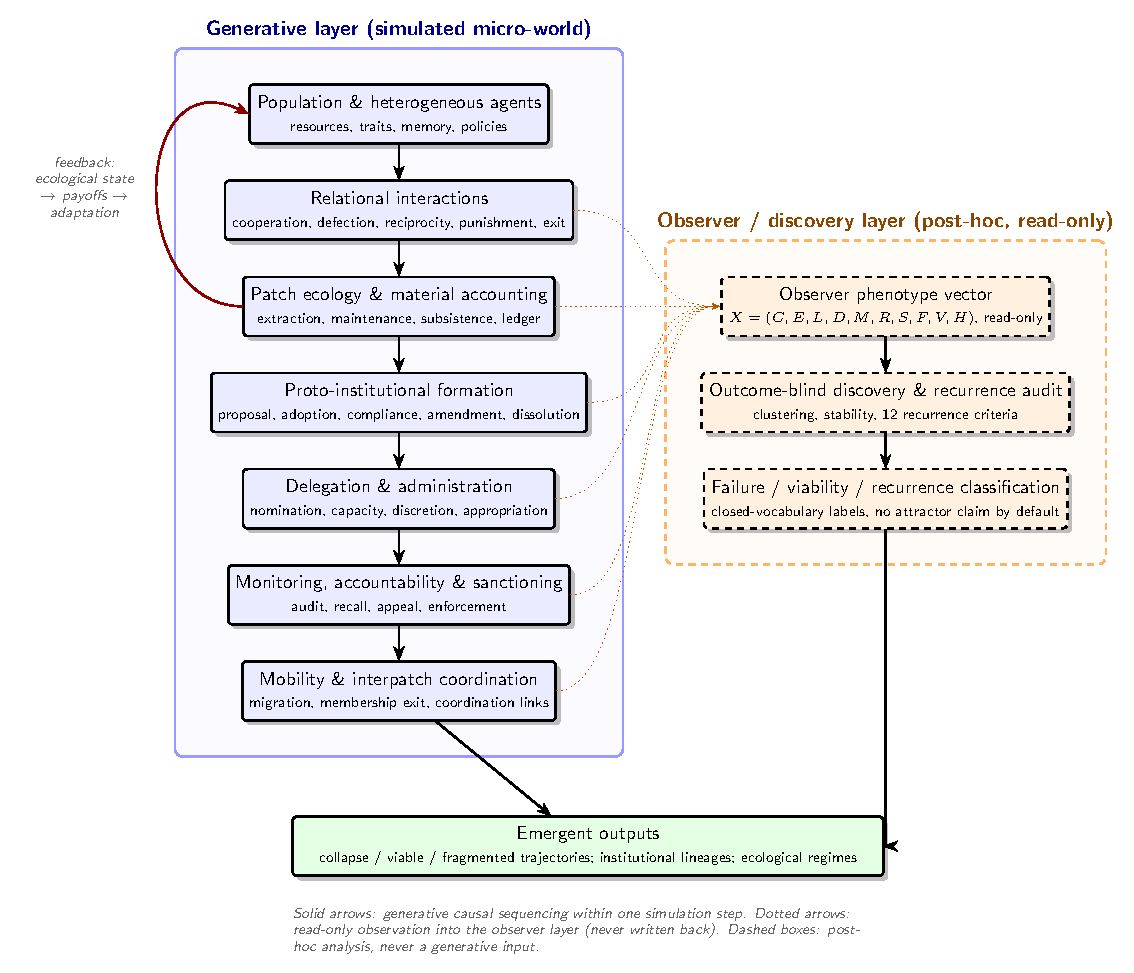
\includegraphics[width=\textwidth]{figures/main/conceptual_framework.pdf}
\caption{Conceptual framework: the generative layer (population,
relational interactions, patch ecology, proto-institutional formation,
delegation and administration, monitoring/accountability/sanctioning, and
mobility/interpatch coordination) versus the observer/discovery layer
(phenotype vector, outcome-blind discovery and recurrence audit, and
classification), kept structurally and visually separate throughout. Solid
arrows are generative causal sequencing within one simulation step; dotted
arrows are read-only observation into the observer layer, never written
back; the red feedback path is the sole channel by which ecological state
alters subsequent agent behavior. Originally authored for this paper
(\texttt{scripts/conceptual\_framework.tex}), structurally informed by
JUNE-style layered agent-based-model overview diagrams but drawn
specifically from this project's own architecture.}
\label{fig:conceptual-framework}
\end{figure}

\subsection{Agents, patches, resources, and networks}
\label{sec:agents-patches}

The population is heterogeneous by construction: every numeric trait is
drawn independently from its own configured distribution, never shared
across agents. Agents interact bilaterally over a dynamic relationship
network under a repeated cooperation/defection payoff grammar, observe
each other with bounded accuracy, retain a decaying memory of past
partners, and may punish a perceived defector at a cost. A second,
structurally independent action dimension governs each agent's ecological
behavior --- extraction, maintenance investment, or restraint --- directed
at one of a fixed number of local resource patches to which agents are
assigned once, at initialization, by a neutral rule. Each patch has its
own carrying capacity and logistic regeneration; extraction and
maintenance are resource-unit transactions rationed under a documented
allocation rule when simultaneous demand exceeds a patch's capacity to
serve it. Level 1.2 adds a structural mobility primitive
(\texttt{PatchSystem.migrate}) and, gated by their own flags, migration
and voluntary membership exit.

\subsection{Behavioral and institutional adaptation}
\label{sec:behavioral-adaptation}

Agents adapt via imitation (copying a peer's policy with probability
increasing in the peer's relative resource advantage) and low-rate
mutation --- never planning or lookahead. The two behavioral dimensions
(social and ecological) are, in the model's default configuration, given
independent imitation draws; a coupled mode exists but is not the
configuration used in the runs reported here. Institutions adapt on a
slower, structurally distinct channel: a locally shared rule
(\texttt{SharedRule}) is proposed, accumulates support, and is adopted or
rejected by a local threshold process; once active it is monitored,
enforced, and may be amended or dissolved; a dissolved rule's parameters
are retained (not discarded) as the sole source from which a later
reconstruction attempt may mutate. From Level 1.1, a rule may delegate
monitoring, record-keeping, sanction execution, maintenance coordination,
or interpatch communication to a nominated and selected delegate, whose
administrative capacity is built up only from realized task performance
(never assigned as a static trait) and who may exercise discretion ---
appropriation and effort withholding --- subject to accountability
(audit, recall, appeal). From Level 1.2, institutions may also be locally
observed by other patches (with noise, distortion, and delay), transmitted
component-wise across the existing coordination-link graph (with
mutation, recombination, or failure), competed for via migration, and
scaled across jurisdictions that grow, shrink, merge, fragment, or
dissolve.

\subsection{Institutional representation and lineage}
\label{sec:institutional-representation}

Each institution is represented by a fourteen-slot component bundle
(\texttt{InstitutionComponents}: proposal, adoption, contribution,
monitoring, sanction, appeal, recall, delegation, administration,
authority, amendment, memory, succession, coordination), of which twelve
are transmissible across the coordination-link graph and two remain
descriptive-only in this milestone. A full lineage record
(\texttt{InstitutionRecord}) tracks parentage, origin mechanism (fresh
proposal, component transmission, reconstruction, or recombination),
active jurisdiction, amendment history, transmission history, and
extinction time and reason. Lineage identifiers are allocated from a
per-simulation-run counter and are therefore unique only \textit{within}
one seed-run; \cref{sec:level12b} reports a genuine bug this created when
pooling lineage identity across the many independent seed-runs Level 1.2b
introduced, and its fix.

\subsection{Random-number substreams and reproducibility}
\label{sec:rng-substreams}

Every stochastic draw in the codebase passes through one explicit, seeded
random-number generator per run; no module calls an unseeded global
source. From Level 1.1b, an opt-in per-mechanism substream architecture
(\texttt{rng\_mode="mechanism\_substreams"}) is available and is
\textit{mandatory} for every causal (matched-seed) experiment in both
Level 1.2 and Level 1.2b, so that a paired comparison's random draws for
one mechanism are never coupled to another mechanism's own draws under
the same nominal seed. The default \texttt{"legacy\_single\_stream"} mode
remains the exact, byte-for-byte baseline for every non-causal run.

\subsection{Observer metrics and outcome classifications}
\label{sec:observer-metrics}

The observer layer is read-only with respect to the generative layer,
checked by an abstract-syntax-tree-based import-direction test: observer
modules may read logged state and events; they may never write back into
agent state, policies, payoffs, or the random-number stream. Two closed,
non-normative classification vocabularies are used throughout. An
all-outcome classification (\texttt{classify\_all\_outcome}) assigns each
seed-run exactly one of seven labels ---
\texttt{no\_institution}, \texttt{collapse}, \texttt{viable},
\texttt{persistent\_extractive}, \texttt{fragmented}, \texttt{transient},
\texttt{unclassified} --- by first-match-wins rule; every label is always
reported, including zero counts, so that a dominant outcome can never be
silently omitted from a summary. A five-label failure-trajectory
classification (\texttt{classify\_failure\_trajectory}, Level 1.2b only)
distinguishes \texttt{no\_collapse\_observed}, \texttt{transient\_%
dip\_recovered}, \texttt{collapse\_onset\_after\_last\_snapshot},
\texttt{late\_onset\_collapse}, and \texttt{sustained\_collapse} from a
coarse population/ecological-fraction series sampled every ten steps.
Neither vocabulary contains, or is derived from, any dissertation-side
concept.

The observer-only institutional phenotype vector
$X=(C,E,L,D,M,R,S,F,V,H)$ --- realized administrative capacity, effective
constraint, legitimacy (voluntary support), concentration of delegated
authority, institutional memory continuity, administrative appropriation
burden, institutional scale/reach, amendment flexibility, ecological/
demographic viability (two subparts, reported separately), and
within-community heterogeneity --- is computed once per seed-run, never
agent-visible and never a generative input anywhere. A dedicated
Level 1.2b audit (\cref{sec:level12b}) formally checked every dimension's
numerator, denominator, window semantics, missingness condition,
aggregation path, and construct type against six required criteria; no
dimension was removed, and the one genuine transparency gap it found
(inconsistent disclosure of whether a requested time window actually
changed a dimension's value) was fixed additively, without changing any
existing numerator, denominator, or computed value.

\subsection{Outcome-blind discovery procedure}
\label{sec:discovery-procedure}

The unit of analysis is one phenotype vector per seed-run, never per
institution and never per simulation step. Preprocessing compares three
missingness strategies (\texttt{complete\_case}, \texttt{mean\_impute},
\texttt{missingness\_indicator}) rather than silently choosing one, with
standardization always fit on the training split only. Three
structurally different clustering families are fit at every $k$ from 1
through 8 (a disclosed reduction from a fuller candidate menu; $k=1$ is
always fit and never treated specially, and no $k$, including $k=3$, is
privileged): a parametric Gaussian mixture model
\parencite{fraley2002model}, agglomerative hierarchical clustering, and
density-based \texttt{HDBSCAN} \parencite{campello2013density}, which
alone among the three permits unclustered noise points rather than
forcing every observation into some cluster. Model selection reports
silhouette \parencite{rousseeuw1987silhouettes}, Calinski--Harabasz,
Davies--Bouldin, cluster-size balance, and, for the Gaussian mixture,
Bayesian and Akaike information criteria and held-out log-likelihood side
by side, with no single metric deciding. Consensus is assessed via a
pooled co-assignment matrix, the variation of information, bootstrap
stability (resample-with-replacement adjusted Rand index against the
original fit; \cite{hubert1985comparing,benhur2002stability,efron1993bootstrap}),
and pairwise algorithm agreement.

Twelve preregistered recurrence criteria (\texttt{minimum\_cluster\_size},
\texttt{cross\_seed\_recurrence}, \texttt{cross\_algorithm\_support},
\texttt{bootstrap\_stability}, \texttt{co\_assignment\_internal\_%
consistency}, \texttt{distinctness\_from\_noise}, \texttt{missingness\_%
strategy\_robustness}, \texttt{parameter\_condition\_diversity},
\texttt{temporal\_persistence\_of\_members}, \texttt{non\_degenerate\_%
cluster\_fraction}, \texttt{k\_selection\_non\_privileged\_support},
\texttt{independent\_of\_single\_lineage}) are evaluated unconditionally
for every candidate cluster, with no short-circuiting, and combined by
strict conjunction --- a candidate is recurrent only if it passes all
twelve, never a majority. None of the twelve references cluster count or
identity. Level 1.2b's own audit (Work Package H, \cref{sec:level12b})
re-examined every criterion's construct, unit of analysis, and redundancy
under the larger joint design, found and fixed a genuine cross-seed-run
lineage-identifier collision (\cref{sec:institutional-representation}),
and froze a versioned, hashed specification before any discovery result
was seen.

Level 1.2b additionally defines a closed six-label discovery-verdict
vocabulary (\texttt{insufficient\_evidence}, \texttt{failure\_dominated},
\texttt{unstable}, \texttt{one\_config}, \texttt{continuum},
\texttt{multi\_config}), evaluated first-match-wins: whether sample size
and a defined headline $k$ exist at all; whether clustering merely
re-derives the model's own failure/success split; whether either
bootstrap or algorithm-agreement stability clears a 0.3 floor (either is
sufficient, since they measure different kinds of robustness); whether
any $k\geq2$ clears a 0.15 silhouette floor; and, if so, whether three or
more evaluated $k$'s sit within 0.05 silhouette of the best $k$
(\texttt{continuum}) versus a single, clearly dominant peak
(\texttt{multi\_config}). This vocabulary is the direct methodological
response to a documented limitation of silhouette-based model selection
alone: a genuine discrete two-cluster structure and a smooth, gap-free
continuum with one dominant bisection can produce statistically
indistinguishable single-peaked silhouette curves. Neither Level 1.2's
nor Level 1.2b's discovery pipeline can, by itself, prove that a sharp
verdict reflects true discreteness; a \texttt{continuum} verdict is
correspondingly read as evidence of gradedness, not merely as an absence
of a sharp answer.

\subsection{Historical pressure, entrenchment, and legitimacy mechanisms}
\label{sec:historical-mechanisms}
\label{sec:observer-metrics-l13}

Level 1.3 adds history as a generative mechanism, not merely a
richer observer-side measurement. Three pressure channels ---
\textit{security pressure} ($W_t$), \textit{bargaining pressure} ($B_t$),
and \textit{coordination-complexity pressure} ($X_t$) --- are each wired
through two of six candidate transmission primitives shared across
channels: \texttt{pressure\_adjusted\_probability} (a pressure-scaled
adjustment to an existing stochastic decision, e.g.\ monitoring or
sanctioning likelihood) and \texttt{pressure\_adjusted\_scale} (a
pressure-scaled adjustment to an existing continuous quantity, e.g.\
contribution size or delegation scope). Every channel defaults to a
verified no-op; enabling a channel changes only the specific decision or
quantity its own transmission primitives touch, confirmed by regression
test against Level 1.2b's own unmodified behavior at every default setting.
\textit{Institutional entrenchment} is a single additional state variable,
an age-dependent multiplier on the cost or difficulty of amending or
dissolving an active rule, driven by \texttt{entrenchment\_maturation\_%
steps}, itself off/moderate/strong. \textit{Dual legitimacy} extends the
existing legitimacy dimension into two independently accumulated, costly,
and fallible ledgers --- \textit{performance legitimacy} ($L_P$, earned
from realized institutional outcomes) and \textit{procedural legitimacy}
($L_R$, earned from realized procedural/reciprocal fairness) --- each
independently enableable.

The observer layer adds two post hoc composites, $S_{\text{obs}}$ and
$Z_{\text{obs}}$, computed exclusively from existing Level 1.2/1.2b/1.3
observer fields and never read back into the generative layer. $S_{\text{%
obs}}$ is the unweighted mean of five components: \texttt{delegation},
\texttt{administrative\_function}, \texttt{monitoring}, \texttt{interpatch\_%
coordination}, and \texttt{performance\_legitimacy}. $Z_{\text{obs}}$ is
the unweighted mean of three components: \texttt{accountability},
\texttt{bargaining\_participation}, and \texttt{procedural\_legitimacy}.
The two composites share zero component dimensions by construction,
confirmed by direct inspection of \texttt{observer/sz\_obs.py}'s own
constants (\cref{sec:level13b-measurement}). We are explicit that
$S_{\text{obs}}$ and $Z_{\text{obs}}$ are this project's own observer-side
constructs, built without reference to and structurally firewalled from
the dissertation's SEM latent factors $S$ and $Z$; any correspondence
between them is a substantive question this paper's own discussion takes
up (\cref{sec:disc-triangulation}), never an assumption built into either
construction.

\subsection{Sequencing, persistence, and sham-controlled causal intervention}
\label{sec:sequencing-and-intervention}

Level 1.3 tests pressure-channel \textit{ordering} via a matched factorial
crossing onset order (\texttt{security\_first}, \texttt{bargaining\_first},
\texttt{coevolution}) with entrenchment and legitimacy conditions, holding
each channel's total cumulative exposure matched across orderings so that
any observed difference reflects onset timing and sequence, not total
pressure magnitude. Level 1.3b adds a third counterfactual pressure-history
transform, \texttt{equalize\_pressure\_series} (flattening a channel's
realized series to its own mean, preserving cumulative exposure exactly
while destroying temporal shape), alongside the two Level 1.3 already
had (\texttt{remove\_pressure\_history}, \texttt{reverse\_pressure\_%
history}).

Windowed persistence diagnostics (\texttt{observer/historical\_%
persistence.py}, new at Level 1.3b) partition a run's own duration into
early/middle/late/final-sustained windows and compute, per window,
within-window means and variances, early-to-middle and middle-to-late
displacement, a convergence/divergence slope, and a closed five-label
persistence classification (\texttt{transient\_differentiation},
\texttt{historical\_hysteresis}, \texttt{pressure\_dependent\_response},
\texttt{entrenched\_path\_dependence}, \texttt{no\_detectable\_%
differentiation}).

Level 1.3b's own Stage 6 adds a sham-controlled, matched-seed causal
intervention design, the strongest causal evidence this project has
produced for or against historical path dependence. For each of 12 matched
seeds, six arms are compared: a \texttt{no\_intervention\_control}; a
\texttt{sham\_identical\_state\_copy} (the checkpoint/fork machinery
itself, with no history actually altered --- this arm must match the
control byte-for-byte, or the fork machinery, not history, would be
responsible for any divergence seen elsewhere); and four real
interventions (\texttt{pressure\_memory\_only}, \texttt{entrenchment\_%
only}, \texttt{legitimacy\_history\_only}, \texttt{all\_history}), each
resetting or erasing a specific piece of accumulated historical state at a
mid-run checkpoint while leaving the rest of the run's own machinery
untouched. \texttt{core/state\_checkpoint.py} supplies the underlying
\texttt{run\_partial}/\texttt{fork}/\texttt{finish} primitives; a genuine
\texttt{copy.deepcopy}/frozenset-iteration-order bug in an early build of
this machinery was caught by the sham arm's own byte-identical requirement
before any real Stage 6 run completed (\cref{sec:level13b-limitations}),
and fixed by rebuilding each intervention arm fresh from an independent
\texttt{Simulation(config)} construction (already proven byte-identical to
a live fork) rather than forking a live object.

\subsection{Extended decision-gate vocabulary}
\label{sec:decision-gate-extended}

Level 1.3b extends Level 1.2b's own closed six-label discovery-verdict
vocabulary (\cref{sec:discovery-procedure}) to eight labels for the
historical-extension milestones specifically, distinguishing among
possible historical-effect outcomes rather than only discreteness outcomes:
\texttt{no\_effect}, \texttt{pressure\_responsive\_nonhistorical} (responds
to pressure magnitude but not temporal order/history), \texttt{transient}
(differentiation appears but reconverges), \texttt{persistent\_continuum}
(persistent path dependence on a continuous gradient), \texttt{two\_%
families}, \texttt{three\_families}, \texttt{four\_or\_more\_families}, and
\texttt{inconclusive}. This vocabulary was frozen, with an explicit note
that its own discovery pipeline must not be biased toward
\texttt{three\_families} as a default, before any Stage 3+ Level 1.3b run
executed. Ruling out the discrete-family labels (\texttt{two\_%
families}/\texttt{three\_families}/\texttt{four\_or\_more\_families}) reuses
Level 1.2b's own frozen \texttt{classify\_discovery\_verdict} function
unmodified, applied to Level 1.3b's own Stage 7 discrete-candidate fit ---
the same discipline Level 1.3 itself already followed, now extended one
milestone further, so that no discreteness rule was ever authored, or
re-authored, after either milestone's own data was already in hand.

\subsection{Preregistration and confirmation logic}
\label{sec:preregistration-logic}

All four milestones freeze a hashed manifest before Stage/Work-Package
execution begins --- mechanism-activation flags, sample sizes,
discovery-pipeline commitments, recurrence criteria, and
random-number-generator discipline for Level 1.2; feasibility-ratio
definitions, ecological strata, institutional bounds, burn-in windows,
run-count arithmetic, and a confirmation rule for Level 1.2b; pressure-
channel/entrenchment/legitimacy activation ranges, sample sizes, and
stage-by-stage design for Level 1.3; and, for Level 1.3b, the eight
hypotheses of \cref{sec:level13b}, the eight-label decision-gate vocabulary
of \cref{sec:decision-gate-extended}, and an explicit
\texttt{DECISION\_GATE\_DO\_NOT\_PREFER = "F\_three\_families"} note scoped
to mean only that the discovery pipeline's own default must not be biased
toward three families, not that three families is disqualified as a
genuine finding if the evidence actually supports it. Every subsequent
stage script recomputes the manifest's cryptographic hash and refuses to
proceed on any mismatch, making the "never alter the model or rerun a
search merely because the outcome differs from an expected answer"
discipline mechanically checkable rather than a stated intention. Level
1.2b's confirmation rule --- if discovery supports no discrete candidates,
including a \texttt{continuum} verdict, the fresh confirmation sample
replicates the null finding rather than being used to manufacture a
candidate to test --- is inherited unmodified by Level 1.3b's own Stage 8
confirmation design. \Cref{sec:level12b,sec:level13,sec:level13b} report
how this rule was actually applied at each milestone.

Both Level 1.3 and Level 1.3b's own governing specifications were
authored, at length, in an earlier working session whose exact verbatim
text is not recoverable after a later context compaction; every downstream
document (preregistration modules, scientific notes, decision-gate reports)
discloses this explicitly in its own text rather than presenting a
reconstructed hypothesis list or evidence-table schema as a verbatim
transcription. This paper reports the reconstructed hypotheses and
findings the source project itself worked from, with the same disclosure
carried forward rather than smoothed over (\cref{sec:limitations}).

\section{Level 1.2: Initial Open Discovery}
\label{sec:level12}

\subsection{Experimental design}
\label{sec:level12-design}

Level 1.2's own Stage 0 preregistration manifest freezes the discovery
pipeline's commitments (three candidate clustering methods, $k=1$--$8$,
three missingness strategies), the twelve recurrence criteria as a
conjunction, and a mandatory mechanism-substream random-number-generator
mode for every causal run, all before any Stage 1--7 run executed
(\cref{tab:l12-design}).

\begin{table}[htbp]
\centering
\caption{Level 1.2 experimental design by stage.}
\label{tab:l12-design}
\adjustbox{max width=\textwidth}{\begin{tabular}{@{}lrrl@{}}
\toprule
\textbf{Stage} & \textbf{Seeds/draws} & \textbf{Total runs} & \textbf{Purpose} \\
\midrule
1: mechanism activation & 8 seeds $\times$ 7 conditions & 56 & Confirm every mechanism reachable \\
2: small open pilot      & 10 seeds, 1 condition        & 10 & First open-ended exploratory look \\
3: main open search       & 12 draws $\times$ 2 seeds     & 24 & 8-dim Latin Hypercube parameter sweep \\
4: blind discovery        & pools Stage 3               & (24 pooled) & Clustering + 12 recurrence criteria \\
5: prospective confirmation & 12 draws (fresh seeds)     & 12 & Independent replication of Stage 4 \\
6: scaling robustness      & 4 conditions $\times$ 2 seeds & 8 & Population/patch-count scale grid \\
7: perturbation/transition & 2 types $\times$ 3 seeds      & 6 pairs & Shock recovery/transition test \\
13: causal ablations       & 2 factors $\times$ 8 matched pairs & 32 & Matched-seed causal test \\
\bottomrule
\end{tabular}
}
\end{table}

Seven stages followed: mechanism-activation
calibration (Stage 1); a small, single-condition open pilot (Stage 2, $n=10$
seeds); a main open evolutionary search over an eight-dimensional Latin
Hypercube parameter space (Stage 3, 12 parameter draws $\times$ 2 seeds =
24 runs); a blind discovery run over Stage 3's pooled output (Stage 4); an
independent, fresh-seed prospective confirmation using the same 12
parameter draws (Stage 5, $n=12$); a scaling-robustness grid (Stage 6,
population $\in\{40,80\}\times$ patches $\in\{3,6\}$, 8 runs); and a
perturbation/transition test (Stage 7, 6 shocked/unshocked pairs). Section
13 added two matched-seed causal ablations on top of Stages 2--7's purely
correlational findings.

\subsection{Collapse-dominated search}
\label{sec:level12-collapse}

The dominant finding across every stage was near-universal ecological
collapse. Stage 2's ten-seed pilot returned 7 collapse, 3 fragmented, 0
viable. Stage 3's 24-run main search returned 22 collapse, 2 fragmented, 0
viable --- collapse dominated across the swept parameter range, not one
isolated setting (\cref{fig:l12-stage3-outcomes}). Stage 5's fresh-seed
confirmation, reusing Stage 3's own 12 parameter draws, returned 11
collapse and, for the first time in the milestone, 1 viable outcome (draw
9, notably high patch regeneration rate). Stage 6's scaling-robustness
grid returned 8 collapse out of 8 runs across population 40--80 and
3--6 patches (\cref{fig:l12-scaling}) --- ruling out a small-population
artifact as the explanation. Stage 7's perturbation/transition test was
inconclusive by design: both shocked and unshocked baseline conditions had
already collapsed, leaving no non-collapse state for a shock to transition
away from, a disclosed floor effect rather than evidence that
perturbations are inert.

Section 13's two matched-seed causal ablations (\texttt{rng\_mode=%
"mechanism\_substreams"}, 8 seed pairs each) tested the two candidate
explanations Stages 2--7 had only observed correlationally. Toggling
migration on versus off at matched seeds found 5 of 8 pairs favored
migration off on ecological resource fraction (mean paired difference
$-0.077$), with 4 of 8 pairs showing an outcome-label transition (3 of
those 4 moving from \texttt{fragmented} to \texttt{collapse} when migration
was turned on); a Wilcoxon signed-rank test on the paired differences gave
$p=0.25$ \parencite{wilcoxon1945individual}, reported as supplementary
only given the small sample. Toggling the patch regeneration rate between
Stage 3's own sampled bounds (0.2 versus 1.0) found a more consistent
signal: 7 of 8 pairs favored the higher regeneration rate (mean paired
difference $+0.033$), 2 of 8 outcome-label transitions (both
\texttt{collapse}$\to$\texttt{fragmented}), Wilcoxon $p=0.039$. Neither
ablation overturned the headline collapse finding: 13 of 16
migration-ablation runs and 14 of 16 regeneration-ablation runs still
landed in \texttt{collapse}. Both factors are real, causally implicated
contributors; neither is sufficient alone to make \texttt{viable} the
typical outcome at the tested population and duration scale.

\subsection{Null recurrence result}
\label{sec:level12-null}

Stage 4's blind discovery run pooled Stage 3's 24 seed-run phenotype
vectors and evaluated 76 candidate clusters (two clustering methods across
8 values of $k$, plus \texttt{HDBSCAN}'s own clusters) against all twelve
recurrence criteria. Zero of 76 met all twelve
(\cref{fig:l12-recurrence-criteria}); the thirteen best candidates, each
passing eleven of twelve, were uniformly \texttt{hierarchical} $k=6$
partitions dominated by collapse-labeled members, and uniformly failed
\texttt{cross\_algorithm\_support} --- no other clustering method
corroborated that specific partition. Stage 5's independent replication,
on a genuinely fresh, disjoint 12-run pool using the identical, unmodified
discovery pipeline, found the same result: zero of 72 candidates met all
twelve criteria (\cref{fig:l12-discovery-replication}). Held-out
log-likelihood, computed by fitting on Stage 3's own training data and
scoring Stage 5's genuinely held-out fresh runs, degraded gradually from
$k=1$ to $k=3$ and then collapsed catastrophically at $k\geq4$ --- the
textbook signature of small-sample Gaussian-mixture overfitting, and
independent evidence against trusting any higher-$k$ partition from a
sample this size, consistent with the recurrence-criteria result.

Per this milestone's own closing instruction, this is reported exactly as
"the recurrent-phenotype hypothesis was not supported at this sample
size" --- not as evidence against any particular count, not zero, not
one, not three, and not as grounds to alter the model or widen the search
now that the outcome was known.

\subsection{Why ecological confounding required Level 1.2b}
\label{sec:level12-why-1.2b}

Level 1.2's own main pool put 22 to 24 of every 24 runs in
\texttt{collapse}. This licenses a narrower conclusion than "no recurrent
institutional configuration exists in this model": it licenses "within the
sampled region, collapse was the dominant recurrent \textit{system}
outcome, and no recurrent \textit{institutional} configuration was
independently supported" --- because a sample this collapse-saturated
gives a discovery pipeline very little non-collapse institutional
variation to find structure in even if such structure exists. Level
1.2's own completion report states this limitation explicitly: the
eligible, non-collapse subset available to any future discovery attempt
was 2 of 24 runs in Stage 3 and 1 of 12 in Stage 5. Level 1.2b
(\cref{sec:level12b}) exists to close exactly this inferential gap ---
not by re-running Level 1.2's search hoping for a different answer, but
by building an ex-ante ecological feasibility measure, stratifying the
design by it before any institutional variation is sampled, and sampling
at roughly 24 times the scale.

\section{Level 1.2b: Ecologically Stratified Rediscovery}
\label{sec:level12b}

\subsection{Exact accounting and ledger validation}
\label{sec:level12b-ledger}

Before any feasibility ratio could be trusted, Level 1.2b required its own
ecological ledger --- a full supply/demand/net-zero-transfer
reconciliation of total system resources (every patch's stock, every
agent's resources, and every active rule's fund) --- to close to zero
within a documented floating-point tolerance
(\cref{sec:appendix-accounting} gives the full identity and category
list). The ledger was first validated only at short scale (population 16,
3 patches, 40 steps) and marked complete on that basis. While preparing
the milestone's actual production-scale design (population 32, 4 patches,
700 steps), the identical configuration preset showed a residual of
$9.14$, not approximately zero --- the ledger-closure gate blocked the
main discovery run pending investigation, exactly as its own preregistered
stop condition required.

All six root causes shared one property: none could manifest at short
scale. They were, in order of discovery: (1) a sign-flip in every
capped-resource-deduction site, so that a target agent already in a
negative-resource distress state would have resources incorrectly
\textit{restored} rather than further deducted; (2) a monitoring-cost
event stamped onto every violation observed in a round rather than once
per round, double- and triple-counting a cost paid once; (3) a per-active-
link coordination maintenance fee charged every step but previously logged
only when a separately gated activity roll fired, silently under-recording
the fee on steps where it did not; (4) a rule-identifier/patch-identifier
key-space conflation in dissolution routing that could silently corrupt
institutional state via unrelated numeric coincidences; (5) an amendment-
triggered dissolution path that never removed the dissolved rule from the
live registry, leaving a stale entry whose fund kept counting toward
system totals; and (6) a zero-recipient fund-disposition case not treated
as a loss. After all six fixes, the production-scale configuration
reconciles to a residual on the order of $10^{-10}$ for every seed tried
(\cref{fig:l12b-ledger}); across the milestone's full 576-run discovery
design, the maximum observed residual was $5.9\times10^{-9}$ and the mean
$7.1\times10^{-10}$, confirming the fix generalizes across the full design
space rather than only the configuration that first exposed it. These were
genuine accounting bugs, invisible below production scale, found and
fixed by this milestone's own mandatory preflight audit --- not
generative-behavior changes: every fix is either a bookkeeping correction
or a corrected cleanup of already-dissolved state, confirmed
behavior-preserving against the full pre-existing test suite at every step
of the fix sequence.

\subsection{Ex-ante feasibility measures}
\label{sec:level12b-feasibility}

Two ex-ante ecological feasibility ratios were defined and validated
before being used to stratify the main design. The
\textit{structural feasibility ratio} is a pure function of configuration
(no simulation, no randomness): maximum-sustainable-yield regeneration
(patch regeneration rate times capacity over four, the logistic-growth
maximum at half capacity, summed across patches) divided by population
size times the bare mandatory subsistence cost --- deliberately excluding
every discretionary or institutionally contingent cost, so it never
assumes optimistic endogenous cooperation in either direction. The
\textit{expected-pressure ratio} uses the same numerator but adds expected
behavioral extraction demand, evaluated at configured mean trait values
and a preregistered neutral occupancy of one-half. A feasibility-map
experiment (120 runs: a nine-column Latin Hypercube design over ecological
parameters, at least two population/patch-count combinations, institutional
configuration held fixed) validated both ratios against realized ecological
balance. The expected-pressure ratio predicted realized ecological pressure
substantially better than the structural ratio (Pearson $r\approx0.84$
versus $r\approx0.48$; \cref{fig:l12b-feasibility-ratios}), an expected,
un-tuned result given that only the expected-pressure ratio incorporates
behavioral extraction demand. The feasibility map itself returned a
genuinely informative, non-degenerate three-way outcome split (50 other,
52 collapse, 18 saturation out of 120 runs; \cref{fig:l12b-feasibility-strata}).
Tertile cut points on the expected-pressure ratio, computed from this
design's own ecological draws and frozen before any discovery run, define
the three ecological strata (low, medium, high) used to stratify the main
joint design.

\subsection{Stratified experimental design}
\label{sec:level12b-design}

The main discovery design (Work Package E) crosses a freshly sampled
ecological feasibility space with a freshly sampled 21-dimensional
institutional Latin Hypercube design (60 institutional points, verified
free of correlated parameter "packages") and two initial-condition
families --- an institution-free default state, and a heterogeneous
proto-institution injected independently per patch --- stratified only by
the ex-ante expected-pressure ratio, never by any realized simulation
outcome. The preferred design (48 joint points $\times$ 6 seeds
$\times$ 2 initial-condition families = 576 runs) was executed in full: 576
of 576 runs completed with zero failures, stratum spread 17/16/15 points
(204/192/180 runs) across low/medium/high, both initial-condition families
balanced exactly at 288/288, and every run's ledger residual under the
$10^{-4}$ tolerance (\cref{tab:l12-vs-l12b-design} compares this design
directly against Level 1.2's own 24-run design).

\subsection{Discovery and confirmation samples}
\label{sec:level12b-discovery-confirmation}

The main discovery pipeline (Work Package J) reused Level 1.2's own
failure/viability classification unmodified and added a five-label
failure-trajectory classification. On the full 576-run pool: all-outcome
distribution collapse 326, viable 161, fragmented 89, every other label
zero (\cref{fig:l12b-outcome-distribution}); failure-trajectory
distribution sustained collapse 305, no collapse observed 194, transient
dip recovered 56, late-onset collapse 21 --- most collapse outcomes were
sustained across a run's duration, not a last-instant artifact. All 576
runs cleared the non-normative sustained-system data-sufficiency screen,
comfortably above both the preferred (60) and hard-minimum (40) gates.

Clustering and structure discovery (Work Package K) reused Level 1.2's own
primitives unmodified on this much larger pool and reached headline
$k=4$ with verdict \texttt{continuum} (three $k$'s within 0.05 silhouette
of the best; \cref{fig:l12b-discovery-confirmation}). Supporting
diagnostics: bootstrap stability mean adjusted Rand index 0.598 ($k=4$,
30 resamples); mean pairwise algorithm-agreement adjusted Rand index
0.192 (dragged down by \texttt{HDBSCAN} finding zero clusters and 576
noise points on this feature space, while the Gaussian-mixture/
hierarchical pairwise agreement alone was 0.576); missingness-strategy
robustness 0.591 (\texttt{complete\_case}) and 0.653
(\texttt{missingness\_indicator}); cluster assignment essentially
unrelated to initial-condition family (adjusted Rand index 0.0008,
ruling out "clustering is just rediscovering which initial condition a
run started from"); temporal-window stability 0.141 (end-of-run versus
mid-run cluster assignments diverge substantially --- cluster membership
is not stable across a single run's own duration, a genuine finding in
its own right); parameter-neighborhood stability 0.626; and cluster
assignment essentially unrelated to the failure/success split (adjusted
Rand index 0.0, ruling out "clustering is just rediscovering collapse
versus not").

Per the preregistered null-replication rule, a \texttt{continuum} verdict
is treated exactly as a no-candidate finding: no discrete institutional
class was named, bounded, or given an expected direction anywhere in the
confirmation design. What was tested instead was the one concrete object
discovery did produce --- the headline four-cluster partition --- stress-
tested for out-of-sample recurrence on a fresh, disjoint 384-run
confirmation pool (24 joint points $\times$ 8 seeds $\times$ 2
initial-condition families, a disjoint fresh-seed base). The confirmation
pool's own all-outcome distribution (collapse 245, viable 86, fragmented
53) closely tracked the discovery pool's; its own independent clustering
refit reached headline $k=2$, not 4, with verdict \texttt{unstable} (mean
algorithm-agreement adjusted Rand index 0.276, bootstrap mean adjusted
Rand index 0.182, both below the 0.3 stability bar) --- never
\texttt{multi\_config}, so the primary preregistered null expectation
held. Assignment stability between the frozen discovery fit and the
confirmation pool's own independent labels was moderate (adjusted Rand
index 0.527), and feature-profile stability across matched clusters was
high (mean cosine similarity 0.948) --- both consistent with a continuum
rather than either pure noise or a sharply discrete structure. The overall
confirmation verdict was \texttt{null\_replicated}.

\subsection{Cluster stability and held-out replication}
\label{sec:level12b-stability}

\cref{fig:l12b-stability-metrics} summarizes the discovery pool's own
stability diagnostics; \cref{fig:l12b-discovery-confirmation} plots the
discovery and confirmation silhouette curves side by side, visually
showing both the discovery pool's shallow, multi-peaked profile and the
confirmation pool's independent, differently shaped profile --- the
headline $k$ itself is unstable across independent samples, which is
direct evidence for reading the discovery pool's own \texttt{continuum}
verdict as gradedness rather than an artifact of one sample.

A genuine seed-clustered bootstrap (resampling whole ecological-and-
institutional joint-point groups, correctly accounting for the multiple
seeds nested within each point, rather than treating every seed-row as an
independent draw) reproduced the discovery pool's own stability estimate
closely (seed-clustered mean adjusted Rand index 0.591 versus the flat
bootstrap's 0.598), confirming the original result was not an artifact of
a less conservative resampling unit. Bootstrap 95\% confidence intervals
were computed for the headline point estimates: collapse fraction 0.566
[0.526, 0.608] ($n=576$); population-fraction recovery 0.0 [0.0, 0.0]
($n=32$, a tight zero-width interval, itself informative); ecological-
fraction recovery 0.875 [0.75, 0.97]. All four pooled run sets (Work
Packages E, L, M, N) were verified pairwise seed-disjoint.

\subsection{Scale tests and causal ablations}
\label{sec:level12b-scale-causal}

A 32-run scaling-robustness grid (2 population sizes $\times$ 2 patch
counts $\times$ 2 network-modularity levels $\times$ 4 seeds, scale
invariance explicitly not required) found collapse remained dominant at
smaller, structurally varied scales (25 collapse, 4 fragmented, 3 viable;
\cref{tab:outcome-distribution}) and exposed a genuine, disclosed
dissociation between two recovery dimensions after a standardized shock:
population-fraction recovery was 0 of 32 (0\%) at every scale tested,
while ecological-fraction recovery was 28 of 32 (87.5\%). This
dissociation is precisely why no "attractor" label was assigned anywhere
in this milestone: an attractor claim would require majority recovery on
\textit{both} tracked dimensions, and population's own 0\% alone rules it
out (\cref{fig:l12b-causal-ablation} places this alongside the causal
decomposition below; see \cref{sec:appendix-tables} for the full
scaling-robustness table).

A thirteen-factor, 208-run matched-seed causal decomposition (eight
matched-seed pairs per factor, \texttt{rng\_mode="mechanism\_%
substreams"}) moved beyond Level 1.2's own two-factor ablation to test
every major mechanism family's causal contribution to ecological outcome
directly. The two largest ecological-fraction effects were
\texttt{subsistence} (mean paired difference $+0.198$; collapse
probability fell from 1.00 to 0.62 as subsistence cost rose from 0.1 to
0.6 --- counterintuitive, reported as found, not reinterpreted) and
\texttt{migration\_on\_off} (mean paired difference $-0.110$; migration on
worsens the ecological outcome, collapse probability rising from 0.38 to
0.88, directly replicating Level 1.2's own Section 13 migration finding
at roughly 24 times the scale). \texttt{migration\_congestion} and
\texttt{patch\_regen} each contributed a further $\approx+0.11$ and
$+0.10$ respectively. The smallest effect, \texttt{transmission\_cost},
showed essentially no causal signal (mean paired difference $-0.002$,
zero outcome-label transitions in 8 pairs) --- the institutional-
transmission-probability lever this milestone tested does not move
collapse risk in this design. \cref{tab:causal-ablation} reports the full
ranked table; results were never fed back into any already-frozen
artifact, honoring the milestone's own recalibration-prohibition stop
condition.

\subsection{The final continuum/null verdict}
\label{sec:level12b-verdict}

Work Package O's synthesis, applying a closed seven-label cautious
vocabulary and a fixed rule that no "attractor" label may be assigned
without direct evidence of majority recovery on every tracked dimension,
classified the milestone's overall result as \texttt{continuum}, inherited
directly from Work Package K's own discovery verdict, and assigned no
attractor label anywhere. Of six candidate explanations considered for why
cross-run phenotype similarity is observed at all, the evidence was mixed
by design rather than uniform: consistent with temporary (within-run)
similarity and with independent structural convergence (a proxy measure,
not a literal lineage-based test); consistent with environmentally forced
similarity for the three substantial clusters; against measurement
compression (five of eleven raw principal components were needed to reach
90\% explained variance) and against failure-state similarity (adjusted
Rand index against a collapse/non-collapse proxy of 0.0); and
\texttt{shared\_lineage\_persistence} was not evaluated at all, disclosed
explicitly as an evidence gap rather than silently omitted, since
evaluating it would require a fourth full 576-run re-simulation with
per-run lineage identifiers exported, which this milestone judged
low-value given that the continuum and null-replication findings already
independently established that no discrete, well-separated candidate
structure exists for shared ancestry to explain in the first place.

\section{Level 1.3: Historically Structured Open Discovery}
\label{sec:level13}

\subsection{Experimental design}
\label{sec:level13-design}

Level 1.3's own Stage 0 preregistration manifest freezes the historical
mechanisms' activation ranges, the pooled discovery design, and a
mandatory mechanism-substream random-number-generator mode for every
causal run, before any Stage 1 or later run executed. Nine stages
followed: mechanism-activation calibration and a small open pilot
(Stages 1--2); a 72-run matched-seed sequencing/ordering factorial over
six pressure-onset orderings, holding cumulative exposure matched (Stage
3); a 96-run open pressure-history search (Stage 4); a 48-run (16 seeds
$\times$ 3 arms: base, erased, reversed) matched-seed causal counterfactual
on the security-pressure channel (Stage 5); a blind discovery run pooling
Stages 3--5's 216 seed-run phenotype vectors (Stage 6); a 12-run fresh,
disjoint confirmation pool (Stage 7); an $S_{\text{obs}}$--$Z_{\text{obs}}$
coupling analysis pooling all 228 available runs (Stage 8); and a
24-run scale-robustness check (Stage 9). A genuine, disclosed bug (a
two-layer activation-flag defect, this project's own task \#109) was found
and fixed in the pressure-transmission wiring during Stage 1 calibration,
before any Stage 3+ result was collected.

\subsection{Ordering and counterfactual evidence for a real historical effect}
\label{sec:level13-ordering}

Stage 3's 72-run matched factorial, holding each ordering's cumulative
pressure exposure matched, found a real, if modest, ordering-dependent
spread in $S_{\text{obs}}$/$Z_{\text{obs}}$ across the six tested onset
orderings (approximately 6--7.5\% relative spread), descriptive rather
than resampling-based at this milestone (\cref{fig:l13-ordering}). Stage
5's 16 matched seed-triples (base, erased, reversed pressure history,
single security-pressure channel by disclosed design) found a real,
directionally consistent divergence: mean $|S_{\text{obs}}|$ difference
erased-versus-base $\approx0.0027$, reversed-versus-base $\approx0.0116$,
with 1 of 16 and 3 of 16 seeds respectively showing a qualitative shift in
the sequencing vector itself (\cref{fig:l13-counterfactual}). Neither
result was independently resampled with a bootstrap confidence interval at
this milestone --- Level 1.3b's own purpose-designed Stage 3/6
(\cref{sec:level13b}) is the direct confirmatory successor to both.

\subsection{Discovery result and fresh-data reproduction failure}
\label{sec:level13-discovery}

Stage 6's blind discovery run, pooling Stages 3--5's 216 seed-run phenotype
vectors, reached headline $k=2$ with silhouette 0.334 (silhouette by $k$:
0.334, 0.256, 0.285, 0.297, 0.153, 0.196, 0.297 for $k=2$ through 8) and a
bootstrap stability mean adjusted Rand index of 0.917 (30 resamples) ---
a genuinely stable in-sample fit. Two pieces of evidence, however, argue
directly against reading this as a discrete two-family finding. First,
cross-algorithm agreement was only modest (mean adjusted Rand index
$\approx0.291$), and \texttt{HDBSCAN} found zero clusters on this feature
space entirely. Second, and decisively, Stage 7's disjoint 12-run fresh
confirmation pool --- scoring Stage 6's own frozen fit on data it never
saw --- failed to reproduce it: per-run log-likelihood degraded from
$\approx-1.29$ on the training pool to $\approx-6.05$ on the fresh pool, a
sharp collapse, and every one of the 12 fresh points fell into a single
cluster. A further disclosed confound, $\text{cluster\_vs\_source\_stage}$
adjusted Rand index $\approx0.554$, shows the pooled 216-point discovery
sample is not ecologically homogeneous (cluster assignment partially
tracks which of Stages 3/4/5 a point came from), a genuine limitation of a
pooled, not purpose-designed, discovery sample that Level 1.3b's own Stage
4 (\cref{sec:level13b}) was built specifically to avoid.

Applying Level 1.2b's own frozen \texttt{classify\_discovery\_verdict}
function unmodified to this evidence, Level 1.3's formal six-way
classification is \texttt{D\_continuum}, with \texttt{B\_two\_families}
identified explicitly as the closest runner-up rather than a rejected
alternative --- the same evidentiary caution this paper's own
terminological discipline (\cref{sec:terminology-discipline}) requires.

\subsection{\texorpdfstring{The $S_{\text{obs}}$--$Z_{\text{obs}}$ coupling}{The S\_obs--Z\_obs coupling}}
\label{sec:level13-coupling}

Pooling all 228 runs available across Stages 3, 4, 5, and 7, the observer-
side $S_{\text{obs}}$--$Z_{\text{obs}}$ correlation is strong: Pearson
$r=0.888$ ($p\approx2.4\times10^{-78}$), Spearman $\rho=0.913$
($p\approx3.8\times10^{-90}$), $n=228$ (\cref{fig:l13-coupling}). This is
descriptive and correlational, not yet audited at this milestone for
whether the coupling reflects genuine construct independence, a
shared-construction artifact, or a common behavioral driver --- an open
question Level 1.3 itself explicitly leaves for the next milestone. Stage
9's own coarser check (24 runs across four scale cells) found
$S_{\text{obs}}$ and $Z_{\text{obs}}$ ``qualitatively stable''
($S_{\text{obs}}\in[0.649,0.710]$, $Z_{\text{obs}}\in[0.438,0.470]$), a
suggestive but not dispositive check reported as such rather than as a
formal stability statistic.

\subsection{Why a purpose-designed successor was still required}
\label{sec:level13-why-1.3b}

Level 1.3's own record, audited claim by claim in a dedicated inference
audit before Level 1.3b's own preregistration was frozen, was found free
of fabrication or miscitation, but resting almost entirely on one pooled,
216-to-228-run sample assembled after the fact from Stages 3--5, with only
one genuinely independent fresh-data test (Stage 7's 12 points) --- exactly
the one claim that failed to reproduce. \Cref{sec:level13b} reports the
purpose-designed, preregistered, causally instrumented successor this
motivates.

\begin{figure}[htbp]
\centering
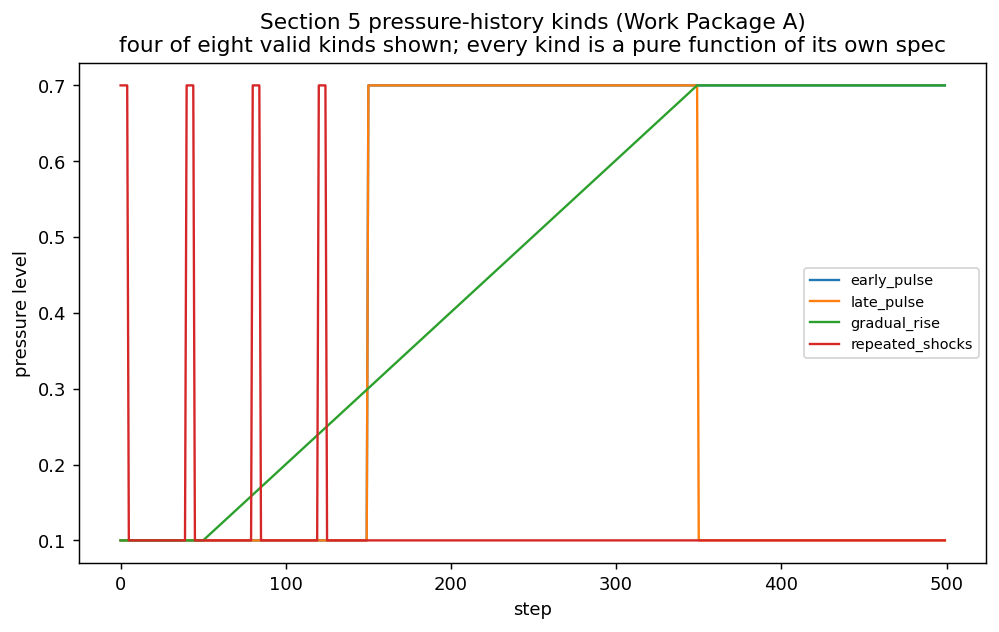
\includegraphics[width=0.85\textwidth]{figures/appendix/a_l13_pressure_history_kinds.png}
\caption{Level 1.3's three pressure channels (security, bargaining,
coordination-complexity) and the pressure-history transforms (base,
erased, reversed) used in Stage 5's matched-seed counterfactual design.}
\label{fig:l13-ordering}
\end{figure}

\begin{figure}[htbp]
\centering
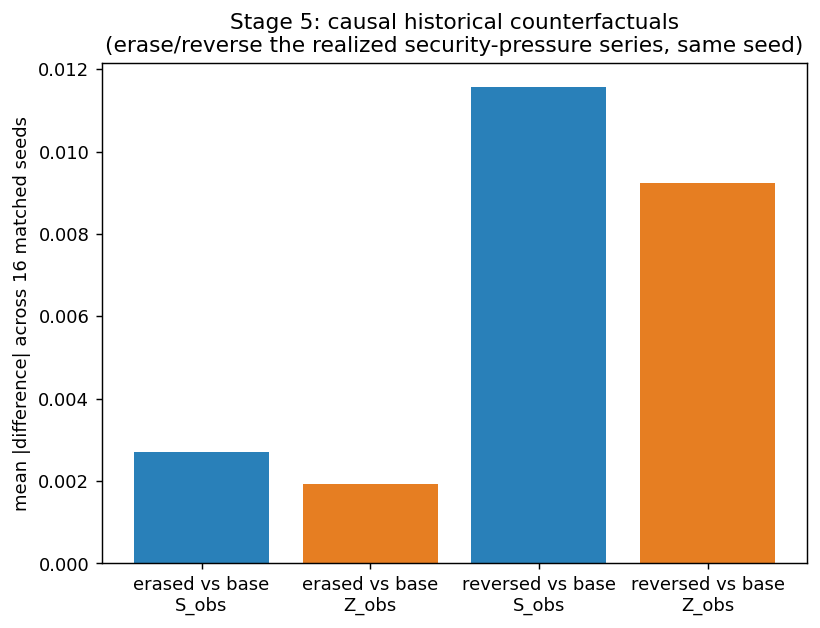
\includegraphics[width=0.85\textwidth]{figures/appendix/a_l13_counterfactual_shift.png}
\caption{Level 1.3 Stage 5: matched-seed counterfactual shift in
$S_{\text{obs}}$/$Z_{\text{obs}}$ for erased and reversed pressure history
versus the base run (16 matched triples, security-pressure channel only).
Descriptive, single-channel; not yet resampled with a bootstrap CI at this
milestone.}
\label{fig:l13-counterfactual}
\end{figure}

\begin{figure}[htbp]
\centering
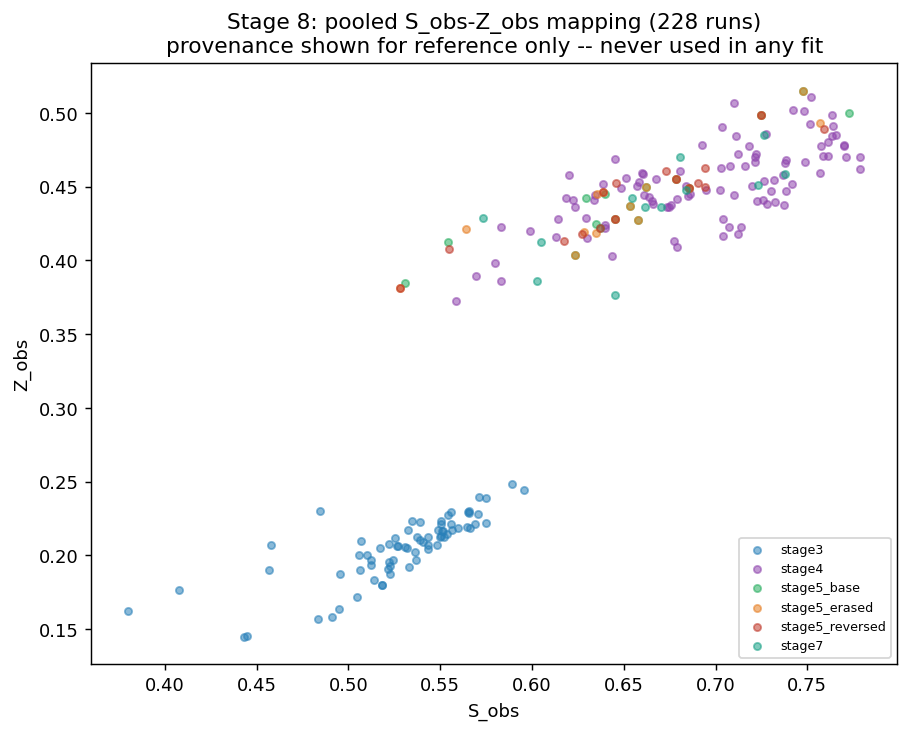
\includegraphics[width=0.85\textwidth]{figures/level13b/l13_fig1_s_obs_z_obs_scatter.png}
\caption{Level 1.3 Stage 8: $S_{\text{obs}}$ versus $Z_{\text{obs}}$ across
all 228 pooled runs (Stages 3/4/5/7). Pearson $r=0.888$, Spearman
$\rho=0.913$. Descriptive correlation; construct-independence audit
deferred to Level 1.3b Stage 9 (\cref{sec:level13b-measurement}).}
\label{fig:l13-coupling}
\end{figure}

\section{Level 1.3b: Purpose-Designed Validation and Causal Intervention}
\label{sec:level13b}

\subsection{Experimental design and eight preregistered hypotheses}
\label{sec:level13b-design}

Level 1.3b's own preregistration manifest freezes eight hypotheses (H1--H8
below), the eight-label decision-gate vocabulary
(\cref{sec:decision-gate-extended}), and a purpose-designed, not
pooled-post-hoc, stage sequence, before any Stage 3+ run executed. Eleven
stages (Stage 0--10) followed, summarized here with their run counts:
Stage 0, frozen-compatibility and cross-process determinism checks (35
comparison runs); Stage 1, a hand-computed microcase plus two
representative runs; Stage 2, a 96-run ($24\times4$) bargaining-activation
calibration sweep; Stage 3, a 216-run purpose-designed matched factorial
(3 orderings $\times$ 3 entrenchment levels $\times$ 4 legitimacy
conditions $\times$ 3 ecological strata $\times$ 2 seeds); Stage 4, a
240-run homogeneous discovery pool; Stage 5, 80 runs (16+16+48) of
persistence classification and counterfactual-persistence diagnostics;
Stage 6, 72 runs (12 seeds $\times$ 6 arms) of sham-controlled causal
intervention; Stage 7, a model-comparison fit reusing Stage 4's own pool
(0 new simulation runs); Stage 8, a 96-run disjoint fresh confirmation;
Stage 9, a 240-run deterministic measurement-weighting audit (re-running
Stage 4's own seeds); and Stage 10, a 24-run ecological-control scale
check. \Cref{tab:l13b-design} summarizes the design; \Cref{tab:l13b-hypotheses}
reports every hypothesis's disposition alongside its own headline evidence.

\begin{table}[htbp]
\centering
\caption{Level 1.3b experimental design by stage.}
\label{tab:l13b-design}
\adjustbox{max width=\textwidth}{\begin{tabular}{@{}lll@{}}
\toprule
\textbf{Stage} & \textbf{Purpose} & \textbf{Runs} \\
\midrule
0 & Frozen-compatibility \& cross-process determinism & 35 (20+15 comparison) \\
1 & Hand-computed microcase \& representative runs & 2+1 \\
2 & Bargaining-activation calibration sweep & 96 (24 cells $\times$ 4 seeds) \\
3 & Purpose-designed ordering/entrenchment/legitimacy factorial & 216 \\
4 & Homogeneous discovery pool & 240 \\
5 & Persistence classification + counterfactual persistence & 80 (16+16+48) \\
6 & Sham-controlled causal history-erasure intervention & 72 (12 seeds $\times$ 6 arms) \\
7 & Discrete/continuous/path-dependent model comparison & 0 (refits Stage 4 pool) \\
8 & Disjoint fresh confirmation & 96 \\
9 & Measurement-weighting audit & 240 (deterministic re-run of Stage 4 seeds) \\
10 & Ecological-control scale check & 24 \\
\bottomrule
\end{tabular}
}
\end{table}

\subsection{H1--H2: activation and ordering}
\label{sec:level13b-h1h2}

\textbf{H1 (bargaining activation): supported.} Stage 4's own 240-run
discovery pool found 166/240 (69.2\%) of runs showing a sustained
\texttt{bargaining\_participation} activation under \texttt{repeated\_%
shocks} pressure, with all three ecological strata represented ---
neither near 0\% (the fix not working) nor near 100\% (the manipulation
uninformative). Stage 2's own calibration sweep found 20/24 (83\%) of
cells landing in the target activation range $[0.2, 0.8]$ at the
\textit{unmodified} Level 1.1/1.2b \texttt{contribution\_amount}/%
\texttt{contribution\_period\_steps} defaults --- no generative
recalibration was required. The fix itself was an observer-construction
correction (\cref{sec:level13b-limitations}), not a change to any
generative rule, confirmed by regression test
(\cref{fig:l13b-bargaining-activation}).

\textbf{H2 (ordering effect): weakly supported, with a disclosed
sign-consistency caveat.} Stage 3's 216-run matched factorial pools to
mean $S_{\text{obs}}$ of 0.597 (\texttt{security\_first}), 0.590
(\texttt{bargaining\_first}), 0.591 (\texttt{coevolution}) --- a real but
modest ($\approx1.2\%$ relative) spread; mean $Z_{\text{obs}}$ 0.369,
0.364, 0.366 ($\approx1.4\%$ relative spread). Of 108 matched pairwise
contrasts, 26 (24.1\%) show a seed-clustered bootstrap confidence interval
on the raw $S_{\text{obs}}$ difference that excludes zero, and 35 (32.4\%)
do so for $Z_{\text{obs}}$ --- a real minority effect, not a null.
Direction is not uniform across the three ordering pairs:
\texttt{security\_first} leads \texttt{bargaining\_first} on
$S_{\text{obs}}$ in 27/36 matched cells (fairly consistent), but
\texttt{security\_first} versus \texttt{coevolution} splits 20/36 positive
to 16/36 negative (a near coin flip), and \texttt{bargaining\_first} versus
\texttt{coevolution} splits 14/36 to 22/36 (a mild reversal)
(\cref{fig:l13b-ordering}). Ordering matters in aggregate and for one
specific pairwise comparison with reasonable consistency, but not as a
single, uniform ``earlier-activating channels always dominate'' rule.

\subsection{H3--H4: persistence and entrenchment}
\label{sec:level13b-h3h4}

\textbf{H3 (temporal persistence): genuinely mixed.} Stage 5 Part A's 16
matched-seed per-seed persistence classifications (\texttt{security\_%
first} versus \texttt{coevolution}) find the \textit{majority} outcome
(9/16) is \texttt{transient\_differentiation} --- mid-run divergence that
fades toward the final-sustained window --- with 4/16 \texttt{historical\_%
hysteresis}, 3/16 \texttt{pressure\_dependent\_response}, and 0/16
\texttt{entrenched\_path\_dependence}. \texttt{condition\_rank\_stability}
returned a degenerate $\pm1.0$ for every seed, disclosed as an
under-specified diagnostic at only 2 ranked conditions rather than treated
as informative. Part B's counterfactual-persistence result, asking a
different question (whether erasing/reversing/equalizing the realized
pressure \textit{history} itself produces a lasting gap, not whether two
different orderings stay apart), points the opposite direction: all three
interventions show a nonzero, non-decaying late-window gap versus the base
\texttt{security\_first} run, most tellingly \texttt{equalized} (early-window
gap 0.027 $\to$ final-sustained gap 0.077, growing, not shrinking).
\Cref{sec:level13b-h5h6} reconciles this apparent tension with Stage 6's
own sham-validated evidence.

\textbf{H4 (entrenchment moderation): not supported as a monotonic
dose-response, though the entrenchment mechanism itself works exactly as
designed.} Stage 3's pooled entrenchment-index-final-step increases
monotonically with the frozen setting (off=0.919, moderate=0.930,
strong=0.955), confirming \texttt{entrenchment\_maturation\_steps} drives
faster accumulation as intended. But mean $S_{\text{obs}}$ across the same
three conditions is 0.594 (off), 0.598 (moderate), 0.586 (strong) ---
\textit{not} monotonic. Stage 6's \texttt{entrenchment\_only} intervention
(resetting only \texttt{founding\_step} mid-run, no pressure magnitude
touched) shows a real, persistent divergence from control (mean
$|S_{\text{obs}}|$ gap: early 0.0, middle 0.017, late 0.065, final-sustained
0.072 --- the \textit{largest} final-sustained gap of the four real
interventions) --- evidence that entrenchment causally matters and
persists, but as a causal presence/absence effect, not the graded
off/moderate/strong dose-response H4 as stated actually claims.

\subsection{H5--H6: sham-validated causal history effect and legitimacy}
\label{sec:level13b-h5h6}

\textbf{H5 (history matters causally): supported, and the sham control did
real work.} Stage 6's sham machinery validation passed exactly: 12/12
seeds' \texttt{sham\_identical\_state\_copy} outcome matches
\texttt{no\_intervention\_control} byte-for-byte
(\texttt{sham\_machinery\_validated=true}) --- the fork/resume machinery
itself introduces zero spurious divergence, the precondition for trusting
any other intervention's divergence as historically meaningful
(\cref{fig:l13b-sham}). Against that validated zero baseline, three of the
four real interventions show real, persistent, non-sham divergence:
\texttt{pressure\_memory\_only} (final-sustained gap 0.054),
\texttt{entrenchment\_only} (0.072), \texttt{all\_history} (0.069) --- none
decaying back toward zero from middle to late window. This is the single
strongest piece of evidence in this project's whole record that historical
path dependence is causally real, not an artifact of measurement or
fork-machinery choice.

\textbf{H6 (legitimacy channel effect): supported for $S_{\text{obs}}$/%
$Z_{\text{obs}}$, but substantially, though not entirely, definitional.}
Stage 3's pooled means: \texttt{performance\_legitimacy\_enabled} moves mean
$S_{\text{obs}}$ from 0.522 (disabled) to 0.665 (enabled);
\texttt{procedural\_legitimacy\_enabled} moves mean $Z_{\text{obs}}$ from
0.244 to 0.492. Both effects are large, and Stage 9's own structural-fact
audit (\cref{sec:level13b-measurement}) explains why: \texttt{performance\_%
legitimacy} is literally one of $S_{\text{obs}}$'s five averaged
components, and \texttt{procedural\_legitimacy} is literally one of
$Z_{\text{obs}}$'s three --- so a disabled channel drags the corresponding
composite down partly by construction, not purely through an independent
behavioral mechanism. The performance/procedural distinction the model
implements as two separate, independently costly and fallible ledgers
tracks a real one in the legitimacy literature, between compliance earned
by delivering outcomes and compliance earned by being seen to follow fair
process \parencite{levi1988ruleandrevenue}.
Stage 6's \texttt{legitimacy\_history\_only} intervention (resetting
accumulated legitimacy \textit{scores}, channel left active) shows the
history-specific effect is transient: middle-window gap $\approx0.009$,
final-sustained gap $\approx4\times10^{-12}$ (numerically zero) --- sharply
unlike \texttt{entrenchment\_only}'s persistent 0.072. Legitimacy
\textit{enablement} changes the composite substantially, partly by
construction; legitimacy \textit{history} specifically does not persist
the way pressure-memory or entrenchment history does.

\subsection{H7--H8: fresh replication and discreteness}
\label{sec:level13b-h7h8}

\textbf{H7 (fresh replication): supported by the letter of the comparison,
with an important qualification carried into H8.} Stage 8's 96-run
disjoint fresh confirmation (fresh design seed, fresh simulation seed
range, never overlapping Stage 4's own 240 points) scores Stage 7's frozen
$k{=}1$ and $k{=}8$ Gaussian-mixture fits on fresh, standardized data:
null $k{=}1$ per-run log-likelihood $=-7.82$; leading $k{=}8$ per-run
log-likelihood $=-4.71$; gap $(k8-k1)=+3.11$, positive --- clearing H7's
own bar (better than Level 1.3's own $-1.29$-versus-$-6.05$ negative
collapse; \cref{fig:l13b-generalization}). But a positive gap against a
single-Gaussian null is close to mechanically guaranteed for any
non-Gaussian continuous cloud of points and does not, alone, distinguish
genuine discrete families from a flexible continuous density. The frozen
continuous candidate (\texttt{pca\_factor\_continuum}) \textit{also}
generalizes comparably well: reconstruction error 0.618 fresh versus 0.597
in-sample training error, a $\approx3.5\%$ increase --- both the leading
discrete and the leading continuous candidate replicate reasonably this
milestone, unlike Level 1.3's own sharp discrete-model collapse.

\textbf{H8 (discreteness): not supported --- the weight of evidence leans
continuum, and this hypothesis was explicitly licensed to fail.} Five
independent, converging signals argue against genuine discreteness at
$k{=}8$ despite H7's positive gap: (1) BIC for \texttt{gmm\_k1\_to\_8} is
non-monotonic and drops sharply with no upturn at the tested boundary
(1214.3 at $k{=}7$ $\to$ 538.2 at $k{=}8$, the single largest drop in the
sequence, right where the search stopped ---
\cref{fig:l13b-bic}); (2) silhouette never clears a moderate bar
(0.055--0.143 across $k{=}2..8$); (3) \texttt{HDBSCAN} finds only 2
clusters with 41\% of points labeled noise at its most permissive setting,
and zero clusters at every stricter setting; (4) cross-algorithm agreement
is weak once the one non-independent pair (\texttt{gmm\_k1\_to\_8} versus
\texttt{unequal\_covariance\_mixtures}, which reduce to the identical
$k{=}8$ fit, adjusted Rand index $=1.0$) is excluded: every other pair ---
\texttt{gmm} versus \texttt{hierarchical} (0.032), \texttt{gmm} versus
\texttt{hdbscan} (0.357), \texttt{hierarchical} versus \texttt{hdbscan}
(0.016) --- shows weak-to-negligible agreement (\cref{fig:l13b-discreteness}); and
(5) the partition does not reproduce across ecological strata: refitting
independently within each of the three strata gives pairwise adjusted Rand
index $-0.043$ to $-0.014$, essentially zero-to-negative agreement.

\subsection{Decision gate: D\_persistent\_continuum}
\label{sec:level13b-decision-gate}

Reusing Level 1.2b's own frozen \texttt{classify\_discovery\_verdict}
function unmodified on Stage 7's data (headline $k{=}8$; silhouette by
$k$: 0.143, 0.135, 0.100, 0.070, 0.073, 0.088, 0.055 for $k{=}2$ through
8; best bootstrap mean adjusted Rand index 0.752, clearing the 0.3
stability bar): \textbf{verdict \texttt{one\_config}}, reason
\texttt{no\_k$\geq$2\_clears\_silhouette\_0.15 (best=0.055)} --- no
evaluated $k$ reaches even the classifier's own entry-level 0.15
silhouette floor; the best silhouette across the whole tested range, at
$k{=}2$, is 0.143, still short. This is a \textit{more} decisive signal
against discrete structure than Level 1.3's own case (which cleared the
0.15 floor comfortably at 0.334 and needed the classifier's tiebreak to
reach \texttt{continuum}); Level 1.3b's own data does not even require
that tiebreak.

Weighing every stage's own evidence together (A/no-effect and
B/pressure-responsive-nonhistorical ruled out by Stage 3/5/6's causal
evidence; E/F/G discrete-family labels ruled out by the classifier result
above; H/inconclusive not selected because the evidence clearly does
support a specific reading), the live question is C (transient) versus D
(persistent continuum). Stage 5 Part A's own majority result favors C for
the narrow ordering-versus-ordering comparison it tests; every other
persistence-relevant measurement --- Stage 5 Part B's three counterfactual
interventions, Stage 6's sham-validated interventions --- shows a growing,
not shrinking, gap. These are not contradictory: two full, well-formed
historical trajectories can converge toward similar long-run behavior
(the narrower sense in which C holds) while each remains causally shaped
by, and measurably different from, a version of itself with its own
history removed (the sense in which D holds at the overall-milestone
level). The formal verdict is \textbf{\texttt{D\_persistent\_continuum}}
--- the same top-level classification Level 1.3's own decision gate
reached, arrived at via a substantially different, independently collected
evidentiary path, and reported here as an observation only, not as
corroborating evidence for D, per this milestone's own stopping-rule
requirement not to silently promote Level 1.3's prior verdict.

\subsection{\texorpdfstring{Measurement audit: the nature of the $S_{\text{obs}}$--$Z_{\text{obs}}$ coupling}{Measurement audit: the nature of the S\_obs--Z\_obs coupling}}
\label{sec:level13b-measurement}

Stage 9's measurement-weighting audit (240 runs, a deterministic re-run of
Stage 4's own seeds) reports the $S_{\text{obs}}$--$Z_{\text{obs}}$
correlation under multiple defensible weighting variants rather than
redefining the measure to manufacture independence or coupling, per this
milestone's own frozen rule: raw/equal-weight $r=0.264$; partial
correlation controlling ecological stratum $r=0.272$; between-point
$r=0.285$; within-point $r=0.261$; leave-one-component-out range
0.175--0.307. One variant is a genuine outlier rather than a small
perturbation: an equally defensible \textit{PCA-weighted} alternative
gives $r=0.136$, roughly half the equal-weight figure
(\cref{fig:l13b-coupling-robustness}). Zero shared component dimensions
between $S_{\text{obs}}$ (5 components) and $Z_{\text{obs}}$ (3 components)
were confirmed by direct inspection of \texttt{observer/sz\_obs.py}'s own
constants. A data-driven factor-structure analysis does \textit{not}
cleanly recover the intuitive $S$/$Z$ axis split: the first principal
component (22.8\% of variance) is loaded by \textit{both} legitimacy
channels together (0.654 \texttt{performance\_legitimacy}, 0.674
\texttt{procedural\_legitimacy}) rather than one loading on an ``$S$
axis'' and the other on a ``$Z$ axis,'' and the scree is flat (seven
components between 7.7\% and 22.8\%, top-two cumulative only 40.9\%).

We state plainly what this does, and does not, license. The coupling is
real, not an artifact of shared construction (zero shared dimensions,
confirmed directly), and it corroborates, in the weak sense of ``these two
observer-side composites move together more than chance,'' the
dissertation's own intuition that state capacity and institutional
constraint are related dimensions of a single governance space. It does
\textit{not} license treating $S_{\text{obs}}$ and $Z_{\text{obs}}$ as the
same construct, does not license claiming the ABM's own observer space
collapses to one dimension, and --- because $S_{\text{obs}}$/$Z_{\text{obs}}$
are this project's own post hoc composites, structurally firewalled from
and never validated against the dissertation's SEM latent factors ---
does not license any claim that this coupling statistically confirms the
dissertation's own $S$/$Z$ correlation, which the dissertation itself never
reports as a single coefficient (\cref{sec:disc-triangulation}).

\subsection{Nulls, anomalies, and disclosed limitations}
\label{sec:level13b-limitations}

Two nulls are reported directly rather than omitted. \texttt{response\_%
cost} (\texttt{contribution\_amount}) had zero measurable effect on
bargaining activation across $[0.02, 0.2]$ (Stage 2) --- resources are
already too deeply negative post-collapse for the ask size to matter;
activation is instead driven by the interaction of \texttt{contribution\_%
period\_steps} and \texttt{sequencing\_min\_duration\_steps}.
\texttt{condition\_rank\_stability} returned a degenerate $\pm1.0$ for
every Stage 5 seed, an under-specified diagnostic at only 2 ranked
conditions, not an informative result. One anomaly bears directly on H8:
\texttt{gmm\_k1\_to\_8} and \texttt{unequal\_covariance\_mixtures} agree
with adjusted Rand index exactly 1.0 because both reduce to the identical
underlying fit at the leading $k$, not because they are independent
corroborating evidence, and \cref{sec:level13b-h7h8} treats it accordingly.

Two source-layer bugs were found and fixed mid-milestone, neither
contaminating any reported result. A cross-process frozenset-hash
non-determinism (\texttt{rules/transmission.py}'s
\texttt{TRANSMISSIBLE\_COMPONENT\_NAMES}, introduced at Level 1.2, invisible
to every prior single-process compatibility check, found only when Stage
0 compared 15 genuinely separate process launches for the first time: 15
distinct outputs pre-fix, 1 identical output post-fix) was fixed by
sorting the union before tupling. A \texttt{copy.deepcopy}/frozenset-
iteration-order defect in Stage 6's own new checkpoint machinery was
caught by the sham arm's own byte-identical requirement on its first smoke
check (0/1 seeds matched) before any real Stage 6 run completed, root-caused
via RNG-call-log instrumentation, and fixed by rebuilding each intervention
arm fresh rather than forking a live object. No conclusion anywhere in
this paper is drawn from pre-fix data for either bug.

The bargaining-activation repair itself (H1) traces to an
\textit{observer-construction} defect --- a zero-fill-versus-forward-fill
bug in \texttt{observer/sequencing\_diagnostics.py}'s own compliance-series
construction, colliding with \texttt{min\_duration\_steps=10} equal to
\texttt{contribution\_period\_steps=10} --- not a generative recalibration;
a second, genuine finding (willingness/solvency conflation under resource
collapse) was disclosed alongside the fix rather than folded into it
silently. Every stage ran at a disclosed, session-budget-scaled
\textit{minimum} sample size stated in the frozen manifest (Stage 4: 240 of
a preferred 432--768; Stage 8: 96 of a preferred 144--288), not adjusted
after seeing results. Stage 5's persistence diagnostics and Stage 6's
history-erasure interventions both operate at one representative cell
(\texttt{entrenchment=moderate}, \texttt{legitimacy=dual},
\texttt{stratum=medium\_feasibility}), not the full Stage 3 factorial.
Stage 8's discrete-versus-continuous fresh-data comparison uses two
metrics that are not on a common scale (log-likelihood versus
reconstruction error), one of the decision gate's own four concrete
``what would change this verdict'' items (\cref{sec:limitations}).

\begin{table}[htbp]
\centering
\caption{Level 1.3b: eight preregistered hypotheses, headline evidence, and disposition.}
\label{tab:l13b-hypotheses}
\adjustbox{max width=\textwidth}{\begin{tabular}{@{}p{2.4cm}p{6.5cm}p{5.8cm}l@{}}
\toprule
\textbf{Hypothesis} & \textbf{Headline evidence} & \textbf{Key caveat} & \textbf{Disposition} \\
\midrule
H1: bargaining activation & 166/240 (69.2\%) Stage 4 activation; 20/24 (83\%) Stage 2 cells in target range at unmodified defaults & Repair was an observer-construction fix, not a generative recalibration & Supported \\
H2: ordering effect & 24.1\%/32.4\% of 108 Stage 3 contrasts CI-significant on $S_{\text{obs}}$/$Z_{\text{obs}}$ & Direction not uniform across the 3 ordering pairs (27/36, 20/36, 14/36 positive) & Weakly supported \\
H3: temporal persistence & Stage 5A majority (9/16) transient; Stage 5B/6 counterfactual gaps grow, not shrink & Two different questions (ordering-vs-ordering vs.\ history-vs-erased-history) answered differently & Mixed \\
H4: entrenchment moderation & Entrenchment index rises monotonically (0.919/0.930/0.955); $S_{\text{obs}}$ does not (0.594/0.598/0.586) & Mechanism works; dose-response on the composite does not & Not supported (as stated) \\
H5: history matters causally & Sham validated 12/12; 3 of 4 real interventions show growing final-sustained gaps (0.054--0.072) & Single representative cell only, not the full Stage 3 factorial & Supported \\
H6: legitimacy channel effect & S/$Z_{\text{obs}}$ shift 0.522$\to$0.665 / 0.244$\to$0.492; legitimacy-history effect decays to $\approx$0 & Legitimacy is a literal component of the composite it is measured against & Supported, construction-driven \\
H7: fresh replication & Stage 8 gap $+3.11$ (vs.\ Level 1.3's $-1.29$-to-$-6.05$) & Continuous candidate also generalizes well; not on its own a discreteness signal & Supported (literal bar) \\
H8: discreteness & BIC leads at $k{=}8$ but silhouette never clears 0.15; weak cross-algorithm (0.016--0.357) and cross-stratum ($-0.043$ to $-0.014$) agreement & Explicitly licensed to fail even if H1--H7 hold & Not supported \\
\bottomrule
\end{tabular}
}
\end{table}

\begin{figure}[htbp]
\centering
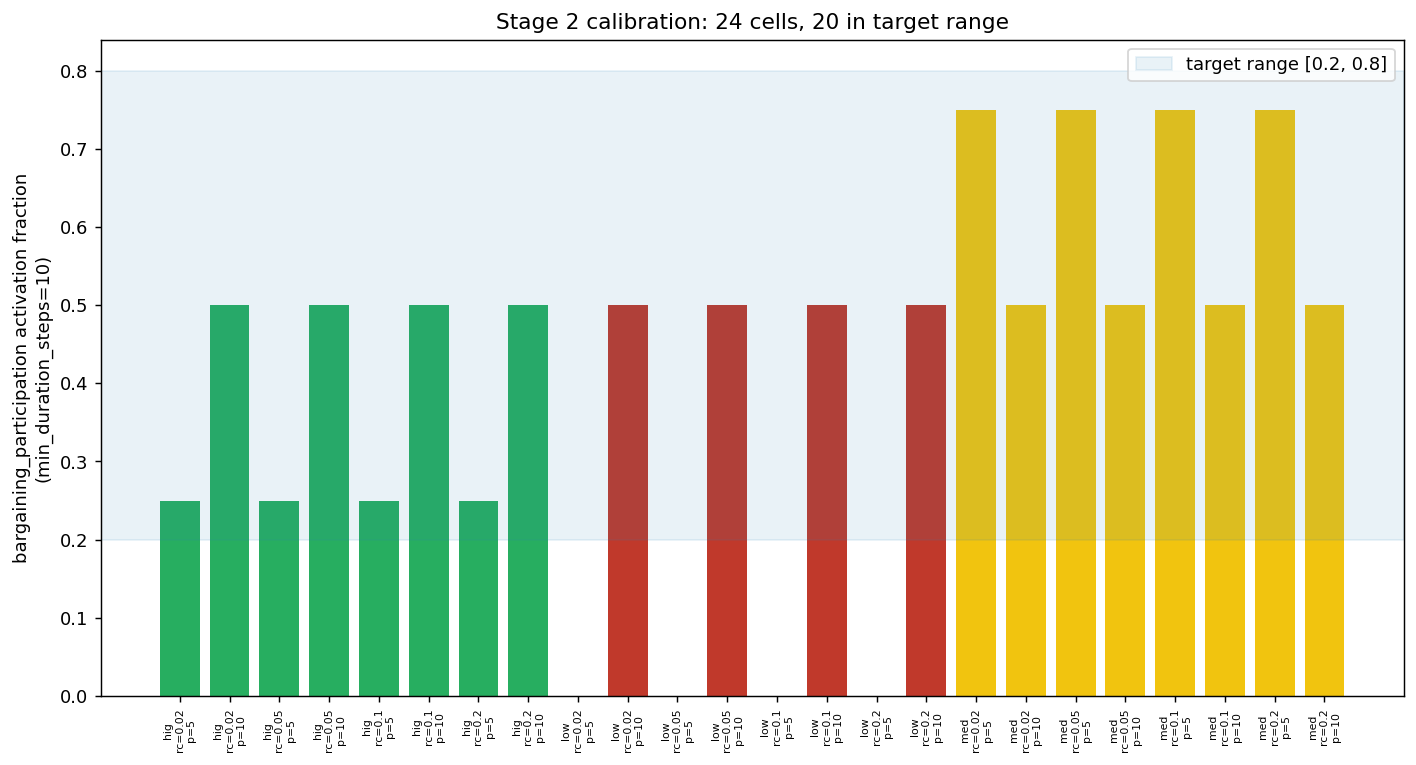
\includegraphics[width=0.75\textwidth]{figures/level13b/l13b_fig2_bargaining_activation.png}
\caption{Level 1.3b H1: bargaining-participation activation after the
Work Package B observer-construction fix. Stage 2 calibration (96 runs,
24 cells $\times$ 4 seeds): 20/24 cells land in the target $[0.2,0.8]$
activation range at unmodified Level 1.1/1.2b defaults.}
\label{fig:l13b-bargaining-activation}
\end{figure}

\begin{figure}[htbp]
\centering
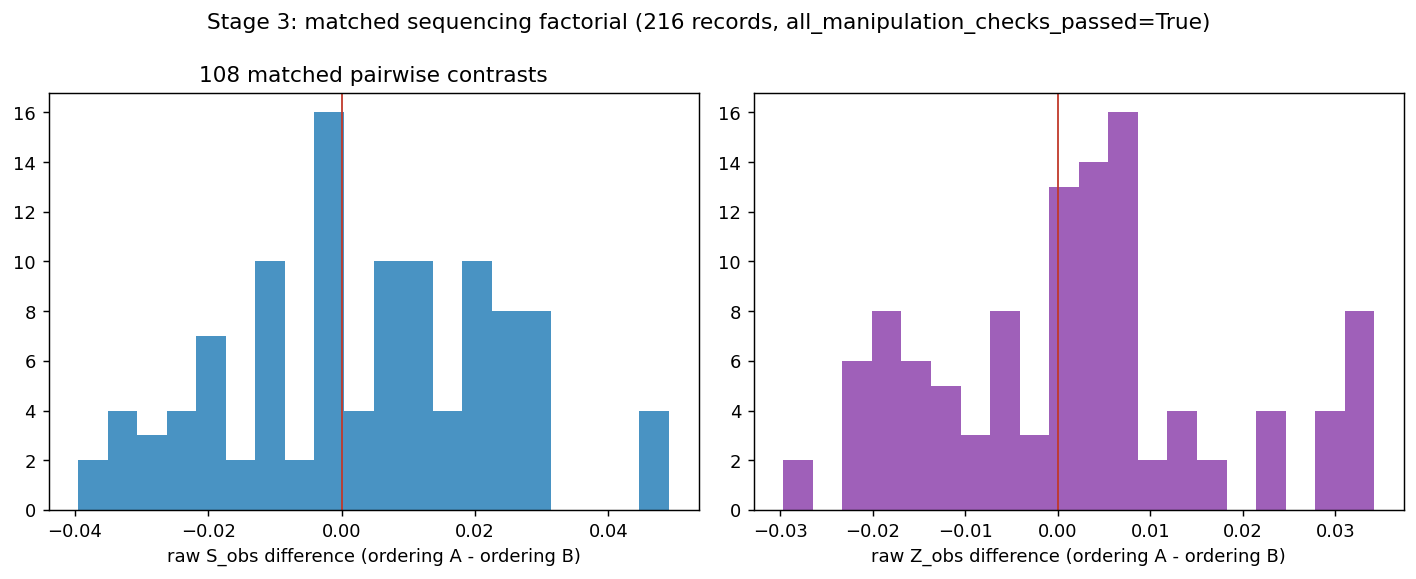
\includegraphics[width=0.85\textwidth]{figures/level13b/l13b_fig3_ordering_contrasts.png}
\caption{Level 1.3b H2: Stage 3 matched pairwise contrasts (216 runs, 108
matched pairwise comparisons per outcome variable), seed-clustered
bootstrap confidence intervals. 24.1\%/32.4\% of contrasts exclude zero on
$S_{\text{obs}}$/$Z_{\text{obs}}$; direction is not uniform across the
three ordering pairs.}
\label{fig:l13b-ordering}
\end{figure}

\begin{figure}[htbp]
\centering
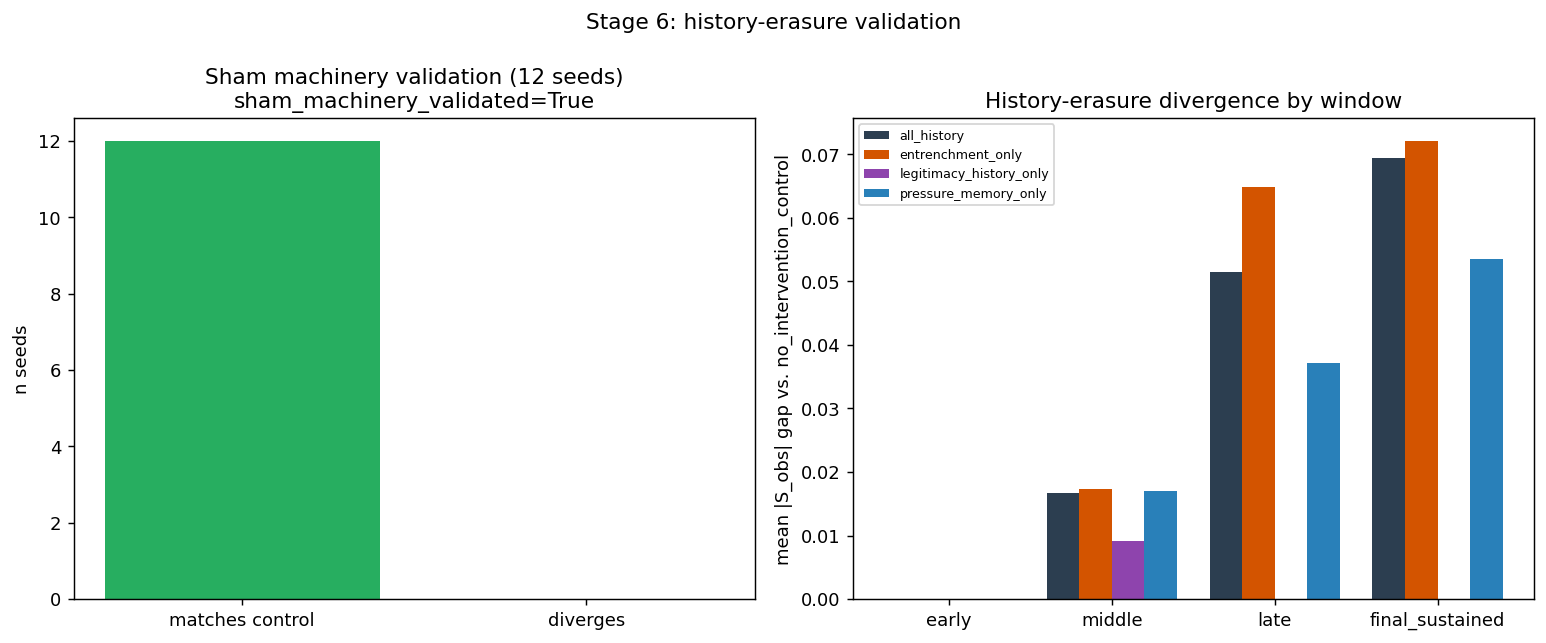
\includegraphics[width=0.9\textwidth]{figures/level13b/l13b_fig4_sham_and_divergence.png}
\caption{Level 1.3b H5: Stage 6 sham-machinery validation (left; 12/12
seeds byte-identical to control) and history-erasure divergence by window
(right; mean $|S_{\text{obs}}|$ gap versus control, four intervention arms
across early/middle/late/final-sustained windows). Every real intervention
except \texttt{legitimacy\_history\_only} shows a growing, non-decaying
gap. Causal evidence, sham-validated --- not a correlational sweep.}
\label{fig:l13b-sham}
\end{figure}

\begin{figure}[htbp]
\centering
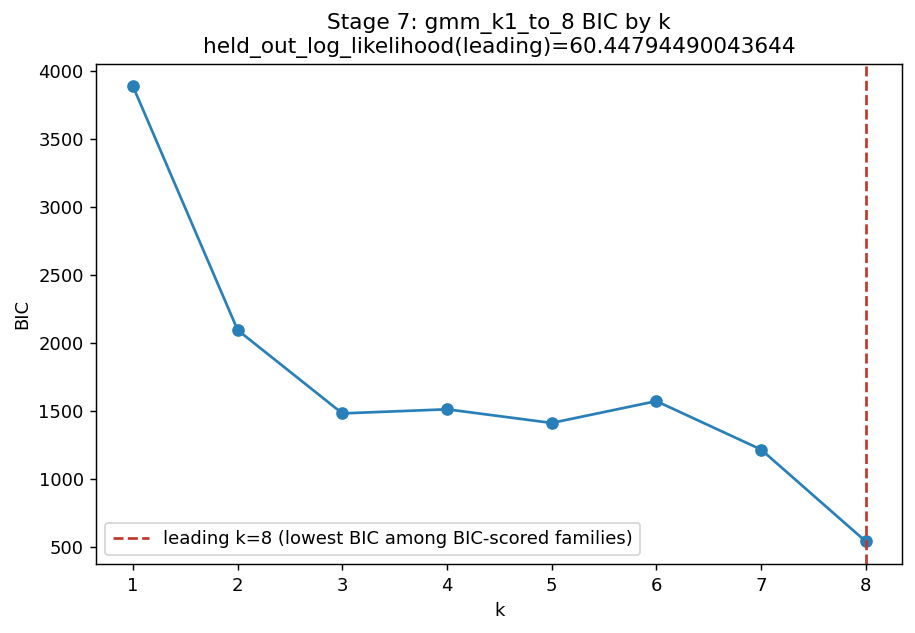
\includegraphics[width=0.75\textwidth]{figures/level13b/l13b_fig5a_bic_curve.png}
\caption{Level 1.3b Stage 7: Bayesian information criterion by $k$ for
\texttt{gmm\_k1\_to\_8} (240 pooled runs). Lowest (``leading'') BIC at
$k{=}8$, with a sharp, non-turning drop from $k{=}7$. \textbf{This BIC
curve alone does not establish eight institutional species}; read only
alongside \cref{fig:l13b-discreteness}'s weak cross-algorithm and
cross-stratum agreement and the silhouette values reported in
\cref{sec:level13b-h7h8}, which together indicate a still-improving
flexible density fit to a continuous, non-Gaussian distribution rather
than eight genuinely separated families.}
\label{fig:l13b-bic}
\end{figure}

\begin{figure}[htbp]
\centering
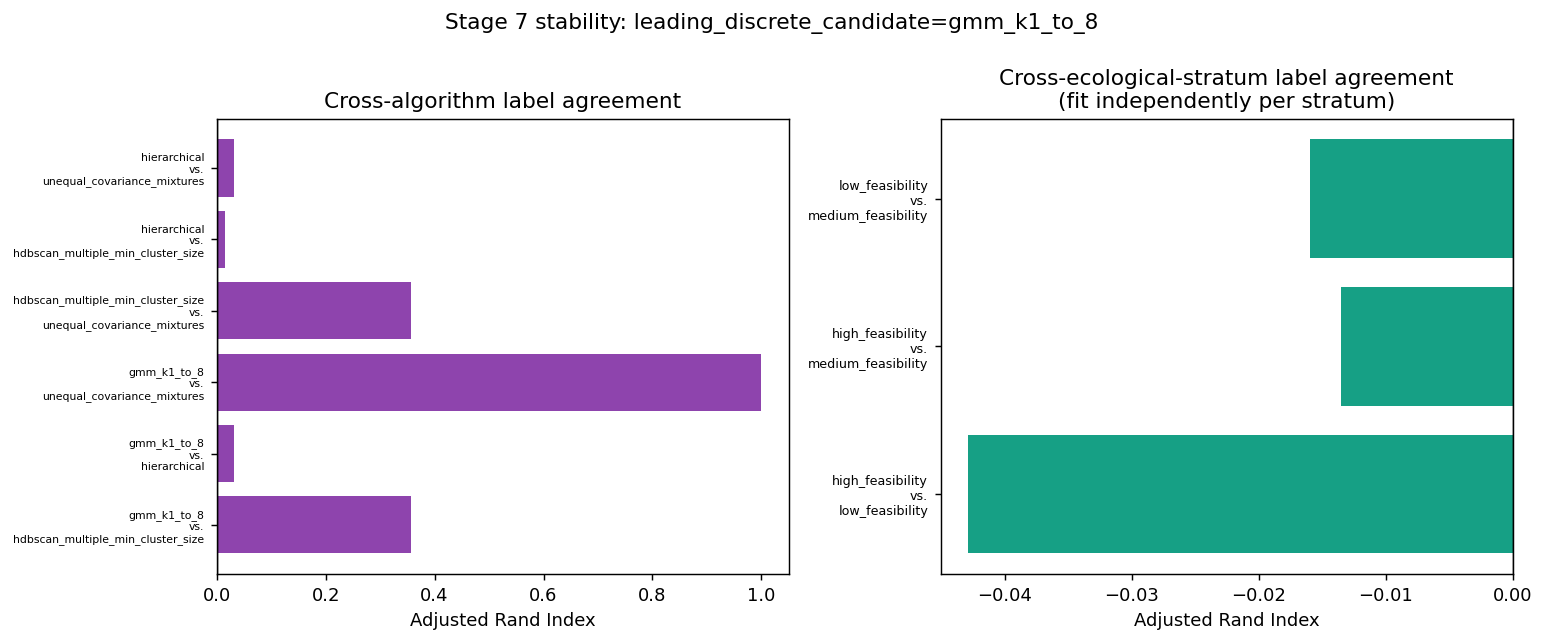
\includegraphics[width=0.95\textwidth]{figures/level13b/l13b_fig5b_discreteness_evidence.png}
\caption{Level 1.3b H8, evidence against discreteness at $k{=}8$: pairwise
cross-algorithm label agreement (left; weak, 0.016--0.357, once the
non-independent \texttt{gmm}/\texttt{unequal\_covariance\_mixtures} pair,
adjusted Rand index 1.0, is set aside) and cross-ecological-stratum label
agreement (right; near-zero to negative, $-0.043$ to $-0.014$, when the
leading method is refit independently within each stratum). Paired with
\cref{fig:l13b-bic} per this paper's own figure-pairing rule: mixture
components are not institutional species.}
\label{fig:l13b-discreteness}
\end{figure}

\begin{figure}[htbp]
\centering
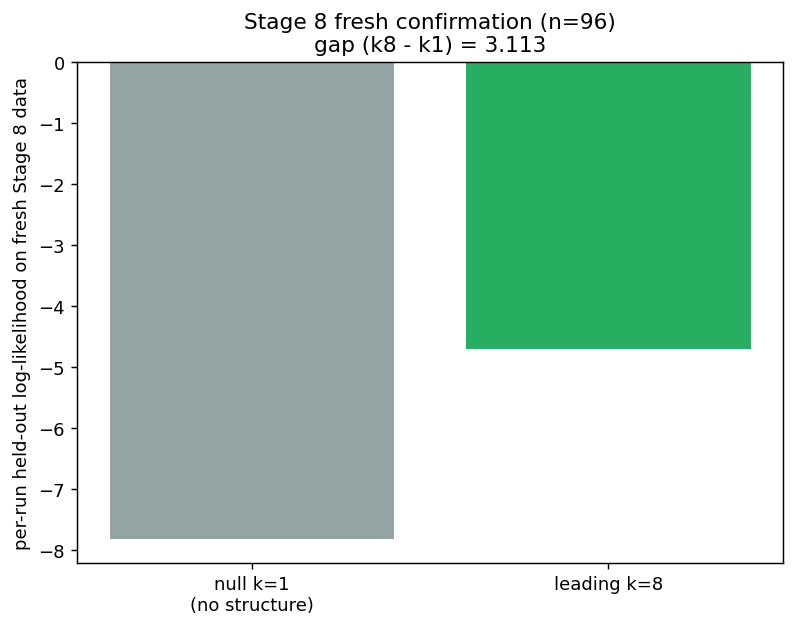
\includegraphics[width=0.6\textwidth]{figures/level13b/l13b_fig6_generalization_gap.png}
\caption{Level 1.3b H7: Stage 8 fresh-data generalization gap, leading
discrete candidate ($k{=}8$) per-run log-likelihood minus null ($k{=}1$)
per-run log-likelihood, 96-run disjoint fresh confirmation pool. Positive
($+3.11$), unlike Level 1.3's own sharply negative fresh-data collapse ---
but a weak discreteness signal alone, since the leading continuous
candidate also generalizes well (\cref{sec:level13b-h7h8}).}
\label{fig:l13b-generalization}
\end{figure}

\begin{figure}[htbp]
\centering
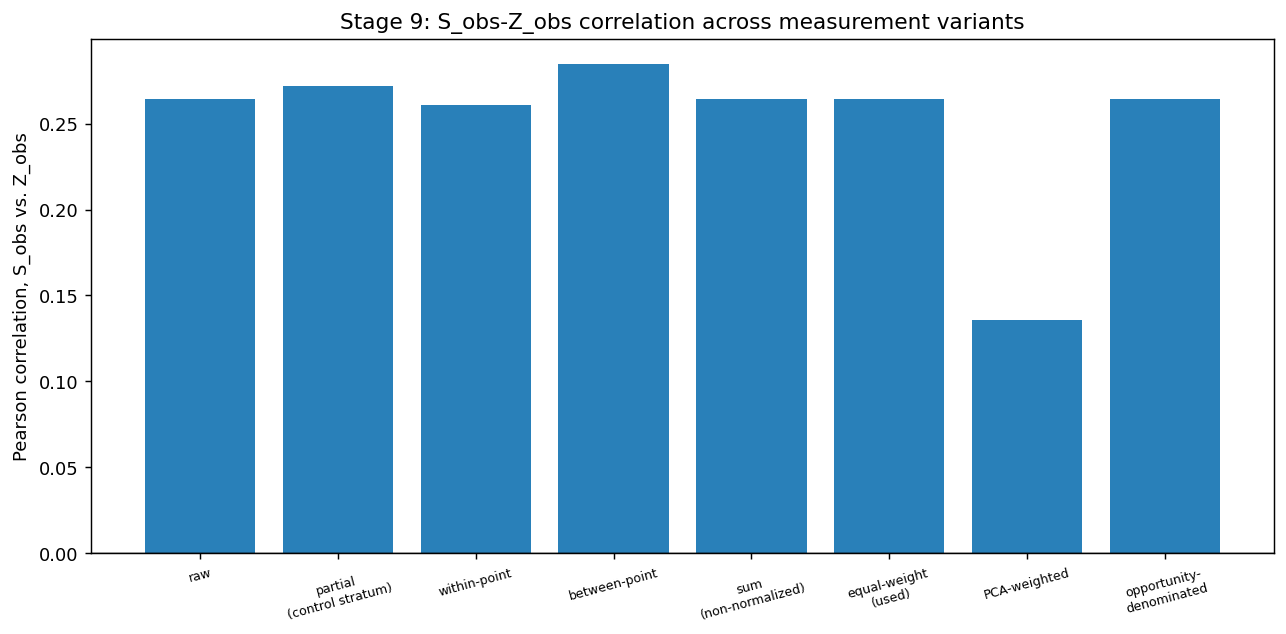
\includegraphics[width=0.85\textwidth]{figures/level13b/l13b_fig7_coupling_robustness.png}
\caption{Level 1.3b Stage 9: $S_{\text{obs}}$--$Z_{\text{obs}}$ correlation
across defensible measurement-weighting variants (equal-weight, partial
controlling ecological stratum, between-/within-point, leave-one-component-
out range, PCA-weighted). Equal-weight and related variants cluster near
$r\approx0.26$--$0.29$; the PCA-weighted alternative is a genuine outlier
at $r\approx0.14$, roughly half.}
\label{fig:l13b-coupling-robustness}
\end{figure}

\section{Results}
\label{sec:results}

This section consolidates the headline quantitative results from all four
milestones (\cref{sec:level12,sec:level12b,sec:level13,sec:level13b}) in
one place; every number below is traceable in \cref{sec:appendix-ledger}
and \texttt{claim\_evidence\_manifest.csv} to its exact source file and
field. \Cref{sec:results-l12,sec:results-l12b-subhead} below reproduce the
synchronic Level 1.2/1.2b results unchanged from the prior milestone;
\Cref{sec:results-l13} adds the historical Level 1.3/1.3b results.

\subsection{Level 1.2 / Level 1.2b: the synchronic substrate}
\label{sec:results-l12}
\label{sec:results-l12b-subhead}

\textbf{Recurrence.} Neither milestone found a recurrent institutional
phenotype structure that survived independent replication. Level 1.2:
0 of 76 candidate clusters met all twelve recurrence criteria at
discovery ($n=24$), and 0 of 72 met all twelve at independent confirmation
($n=12$). Level 1.2b, at roughly 24 times the scale and with explicit
ecological stratification: discovery ($n=576$) reached a \texttt{continuum}
verdict (headline $k=4$, silhouette flat across several $k$, not a single
dominant peak), and independent confirmation ($n=384$, fresh, disjoint
seeds) reached verdict \texttt{unstable} at a different headline $k=2$,
yielding an overall confirmation verdict of \texttt{null\_replicated}
(\cref{tab:recurrence-validation}).

\textbf{Collapse dominance.} Ecological collapse was the plurality or
majority outcome in every pooled sample in both milestones: Level 1.2
Stage 3, 22/24 (91.7\%); Level 1.2b discovery, 326/576 (56.6\%, 95\%
bootstrap CI [52.6\%, 60.8\%]); Level 1.2b confirmation, 245/384
(63.8\%); Level 1.2b scaling grid, 25/32 (78.1\%)
(\cref{tab:outcome-distribution}).

\textbf{Ecological accounting.} The exact ledger closed to a residual on
the order of $10^{-10}$ per seed at production scale after six genuine
accounting bugs (invisible below production scale) were found and fixed,
down from a pre-fix residual of 9.14; across the full 576-run discovery
design the maximum residual was $5.9\times10^{-9}$ against a documented
tolerance of $10^{-4}$.

\textbf{Feasibility ratios.} The ex-ante expected-pressure ratio predicted
realized ecological balance substantially better than the structural
feasibility ratio (Pearson $r\approx0.84$ versus $r\approx0.48$, $n=120$
feasibility-map runs).

\textbf{Scale-dependent recovery dissociation.} After a standardized
shock, population-fraction recovery was 0/32 (0\%) across the
scaling-robustness grid, while ecological-fraction recovery was 28/32
(87.5\%) --- a genuine, disclosed dissociation between two recovery
dimensions, and the direct reason no "attractor" label was assigned
anywhere in either milestone (an attractor claim requires majority
recovery on every tracked dimension).

\textbf{Causal structure of collapse.} A 13-factor, 208-run matched-seed
decomposition found collapse risk causally movable, not fixed: the
largest ecological-fraction effects were \texttt{subsistence} ($+0.198$)
and \texttt{migration\_on\_off} ($-0.110$, migration worsening ecological
outcomes and replicating Level 1.2's own Section 13 finding at larger
scale); the smallest, \texttt{transmission\_cost} ($-0.002$, zero
outcome-label transitions), showed no detectable causal effect
(\cref{tab:causal-ablation}).

\begin{table}[htbp]
\centering
\caption{Level 1.2 versus Level 1.2b: design comparison.}
\label{tab:l12-vs-l12b-design}
\adjustbox{max width=\textwidth}{\begin{tabular}{@{}lll@{}}
\toprule
\textbf{Design element} & \textbf{Level 1.2} & \textbf{Level 1.2b} \\
\midrule
Main discovery sample & 24 runs (12 draws $\times$ 2 seeds) & 576 runs (48 pts $\times$ 6 seeds $\times$ 2 IC families) \\
Confirmation sample & 12 fresh runs & 384 fresh runs (24 pts $\times$ 8 seeds $\times$ 2 IC families) \\
Ecological stratification & none (unstratified sweep) & ex ante, by expected-pressure ratio tertile \\
Ecological ledger validated at production scale & no (short-scale only) & yes; 6 bugs found and fixed, residual $\sim10^{-10}$ \\
Feasibility measure validated against outcomes & no & yes; $r\approx0.84$ (expected-pressure), $r\approx0.48$ (structural) \\
Institutional design dimensions & 8 (parameter-space sweep) & 21 (Latin Hypercube, 60 points, 0 packages) \\
Causal ablation & 2 factors, $n=8$ pairs each & 13 factors, $n=8$ pairs each (208 runs) \\
Scaling-robustness grid & 4 conditions, 2 seeds (8 runs) & 8 conditions, 4 seeds (32 runs) \\
Discovery verdict vocabulary & pass/fail vs.\ 12 criteria only & 6-label closed verdict incl.\ \texttt{continuum} \\
Discovery result & 0/76 candidates meet all 12 criteria & \texttt{continuum} (headline $k$=4) \\
Confirmation result & 0/72 candidates meet all 12 criteria & \texttt{null\_replicated} (headline $k$=2, \texttt{unstable}) \\
\bottomrule
\end{tabular}
}
\end{table}

\begin{table}[htbp]
\centering
\caption{Total generative runs by experimental component.}
\label{tab:run-counts}
\adjustbox{max width=\textwidth}{\begin{tabular}{@{}llrr@{}}
\toprule
\textbf{Milestone} & \textbf{Component} & \textbf{Runs completed} & \textbf{Failures} \\
\midrule
Level 1.2  & Stage 1 (mechanism activation, 7 conditions $\times$ 8 seeds) & 56 & 0 \\
Level 1.2  & Stage 2 (small open pilot) & 10 & 0 \\
Level 1.2  & Stage 3 (main open search) & 24 & 0 \\
Level 1.2  & Stage 5 (prospective confirmation) & 12 & 0 \\
Level 1.2  & Stage 6 (scaling robustness) & 8 & 0 \\
Level 1.2  & Stage 7 (perturbation/transition) & 6 pairs (12) & 0 \\
Level 1.2  & Section 13 (causal ablations, 2 factors) & 16 pairs (32) & 0 \\
\addlinespace
Level 1.2b & Work Package C (feasibility map) & 120 & 0 \\
Level 1.2b & Work Package E/J (main joint discovery) & 576 & 0 \\
Level 1.2b & Work Package L (prospective confirmation) & 384 & 0 \\
Level 1.2b & Work Package M (scaling robustness) & 32 & 0 \\
Level 1.2b & Work Package N (causal decomposition, 13 factors) & 208 & 0 \\
Level 1.2b & Work Package D (secondary-validation classifier, not in headline total) & 20 & 0 \\
\midrule
Level 1.2b & \textbf{Total, 5 main data-generating Work Packages} & \textbf{1,320} & \textbf{0} \\
Level 1.2b & \textbf{Total incl.\ secondary validation} & \textbf{1,340} & \textbf{0} \\
\bottomrule
\end{tabular}
}
\end{table}

\begin{table}[htbp]
\centering
\caption{All-outcome label distribution by pooled run set. Every label is
always reported, including zero counts.}
\label{tab:outcome-distribution}
\adjustbox{max width=\textwidth}{\begin{tabular}{@{}lrrrrrrr@{}}
\toprule
\textbf{Pooled run set ($n$)} & \textbf{no\_inst.} & \textbf{collapse} & \textbf{viable} & \textbf{pers.\ extr.} & \textbf{fragmented} & \textbf{transient} & \textbf{unclass.} \\
\midrule
L1.2 Stage 2 pilot (10)          & --  & 7   & 0   & --  & 3  & -- & -- \\
L1.2 Stage 3 main search (24)     & --  & 22  & 0   & --  & 2  & -- & -- \\
L1.2 Stage 5 confirmation (12)    & --  & 11  & 1   & --  & 0  & -- & -- \\
L1.2b Work Pkg J discovery (576)  & 0   & 326 & 161 & 0   & 89 & 0  & 0 \\
L1.2b Work Pkg L confirmation (384) & 0 & 245 & 86  & 0   & 53 & 0  & 0 \\
L1.2b Work Pkg M scaling (32)     & --  & 25  & 3   & --  & 4  & -- & -- \\
\bottomrule
\end{tabular}
}

\medskip
\noindent\footnotesize ``--'' marks a label not tracked/reported by that
stage's own narrower outcome vocabulary (Level 1.2 Stages 2/3/5 report a
3-label subset; Level 1.2b Work Packages J/L report the full closed
7-label vocabulary with every zero count shown; Work Package M's own
report does not tabulate the 4 unused labels). All values verified
directly against raw JSON output (\texttt{dev\_mem/evidence\_ledger.md},
rows A1--A2, A6, B4, B9, B15).
\normalsize
\end{table}

\begin{table}[htbp]
\centering
\caption{Discovery and confirmation recurrence/cluster validation.}
\label{tab:recurrence-validation}
\adjustbox{max width=\textwidth}{\begin{tabular}{@{}llll@{}}
\toprule
\textbf{Metric} & \textbf{L1.2 discovery} & \textbf{L1.2b discovery} & \textbf{L1.2b confirmation} \\
\midrule
$n$ pooled seed-runs & 24 & 576 & 384 \\
Candidates meeting all 12 criteria & 0 / 76 & --- (\texttt{continuum}, not candidate-based) & --- \\
Headline $k$ & --- & 4 & 2 \\
Discovery/confirmation verdict & n/a (12-criteria only) & \texttt{continuum} & \texttt{unstable} \\
Bootstrap stability (mean ARI) & --- & 0.598 & 0.182 \\
Algorithm-agreement (mean ARI) & --- & 0.192 & 0.276 \\
Overall confirmation verdict & 0/72 candidates (fresh $n$=12) & \multicolumn{2}{c}{\texttt{null\_replicated}} \\
\bottomrule
\end{tabular}
}

\medskip
\noindent\footnotesize ARI = adjusted Rand index \parencite{hubert1985comparing}.
Level 1.2's own pipeline reported only pass/fail against the 12 recurrence
criteria (no closed discovery-verdict vocabulary existed yet); Level
1.2b's six-label verdict vocabulary and stability diagnostics are a
methodological addition, not a retroactive re-analysis of Level 1.2's own
data.
\normalsize
\end{table}

\begin{table}[htbp]
\centering
\caption{Level 1.2b causal-ablation effects on ecological-resource
fraction, ranked by magnitude (Work Package N, 13 factors, $n=208$).}
\label{tab:causal-ablation}
\adjustbox{max width=\textwidth}{\begin{tabular}{@{}lrrrrr@{}}
\toprule
\textbf{Factor} & \textbf{Low} & \textbf{High} & \textbf{Mean paired $\Delta$(eco.\ frac.)} & \textbf{Collapse prob.\ (low$\to$high)} & \textbf{Transitions/8} \\
\midrule
subsistence            & 0.1   & 0.6    & $+0.198$ & $1.00\to0.62$ & 3 \\
migration\_congestion  & none  & 2      & $+0.117$ & $1.00\to0.62$ & 3 \\
migration\_on\_off     & off   & on     & $-0.110$ & $0.38\to0.88$ & 4 \\
patch\_regen           & 0.2   & 1.0    & $+0.102$ & $1.00\to0.62$ & 3 \\
maintenance\_efficiency& 0.3   & 1.0    & $+0.101$ & $0.50\to0.75$ & 6 \\
extraction\_unit       & 2.0   & 10.0   & $-0.080$ & $0.75\to1.00$ & 2 \\
scale\_overload        & 0.0   & 0.2    & $+0.077$ & $0.75\to0.62$ & 2 \\
admin\_cost            & 0.0   & 0.2    & $-0.061$ & $0.62\to0.75$ & 4 \\
capacity               & 200   & 1000   & $+0.036$ & $0.88\to0.75$ & 3 \\
migration\_rate        & 0.05  & 0.4    & $-0.032$ & $0.88\to1.00$ & 1 \\
coordination\_cost     & 0.0   & 0.2    & $-0.027$ & $0.62\to0.75$ & 1 \\
migration\_cost        & 0.0   & 4.0    & $+0.014$ & $0.75\to0.75$ & 2 \\
transmission\_cost     & 0.01  & 0.2    & $-0.002$ & $1.00\to1.00$ & 0 \\
\bottomrule
\end{tabular}
}

\medskip
\noindent\footnotesize Work Package N, 13 factors, 8 matched-seed pairs/factor
(\texttt{rng\_mode="mechanism\_substreams"}), 208 runs total, 0 failures.
Ranked by $|\Delta|$ on ecological-resource-fraction. ``Collapse prob.''
is the fraction of the 8 pairs' low/high arms classified \texttt{collapse}.
Causal evidence (matched-seed design), not a correlational sweep.
\normalsize
\end{table}

\begin{figure}[htbp]
\centering
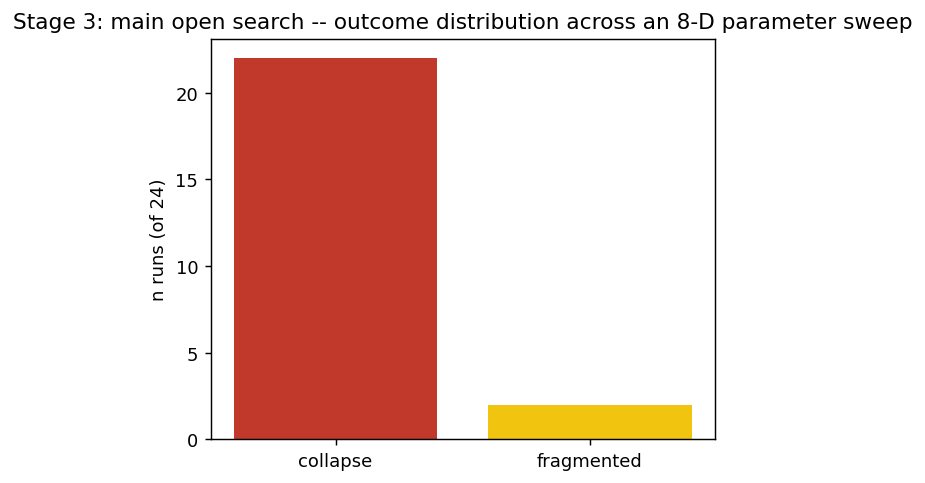
\includegraphics[width=0.75\textwidth]{figures/main/l12_fig1_stage3_outcome_distribution.png}
\caption{Level 1.2 Stage 3 main-search outcome distribution ($n=24$):
22 collapse, 2 fragmented, 0 viable. Descriptive: one run per (parameter
draw, seed) pair from an 8-dimensional Latin Hypercube sweep.}
\label{fig:l12-stage3-outcomes}
\end{figure}

\begin{figure}[htbp]
\centering
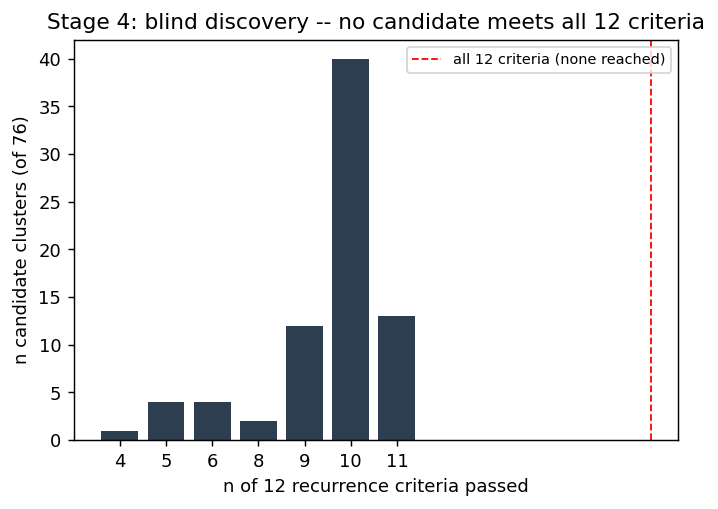
\includegraphics[width=0.75\textwidth]{figures/main/l12_fig2_recurrence_criteria.png}
\caption{Level 1.2 Stage 4: number of the twelve preregistered recurrence
criteria passed by each of 76 candidate clusters ($n=24$ pooled seed-runs).
No candidate passed all twelve; the best passed eleven.}
\label{fig:l12-recurrence-criteria}
\end{figure}

\begin{figure}[htbp]
\centering
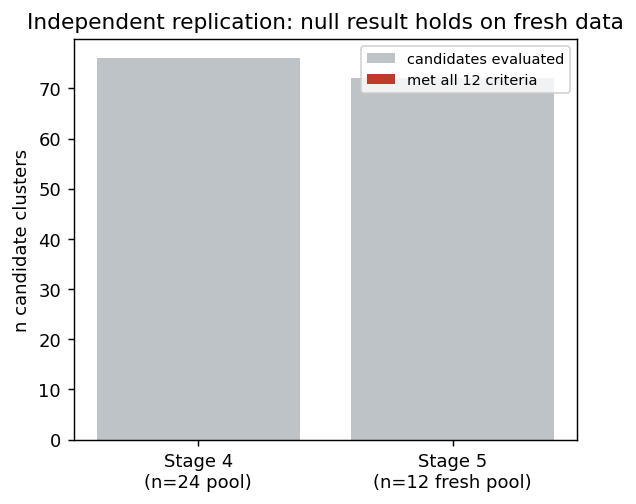
\includegraphics[width=0.85\textwidth]{figures/main/l12_fig3_discovery_vs_replication.png}
\caption{Level 1.2 Stage 4 discovery ($n=24$, 0/76 candidates) versus
Stage 5 independent fresh-seed confirmation ($n=12$, 0/72 candidates),
identical unmodified discovery pipeline. Descriptive null replication.}
\label{fig:l12-discovery-replication}
\end{figure}

\begin{figure}[htbp]
\centering
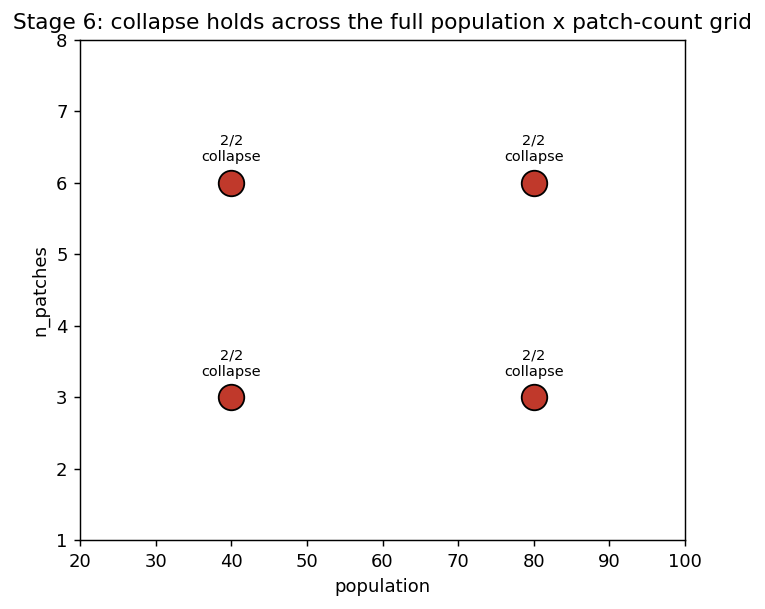
\includegraphics[width=0.8\textwidth]{figures/main/l12_fig4_scaling_grid.png}
\caption{Level 1.2 Stage 6 scaling-robustness grid: outcome label by
population $\times$ patch-count condition (8 runs, 2 seeds/condition).
Collapse in 8/8 runs.}
\label{fig:l12-scaling}
\end{figure}

\begin{figure}[htbp]
\centering
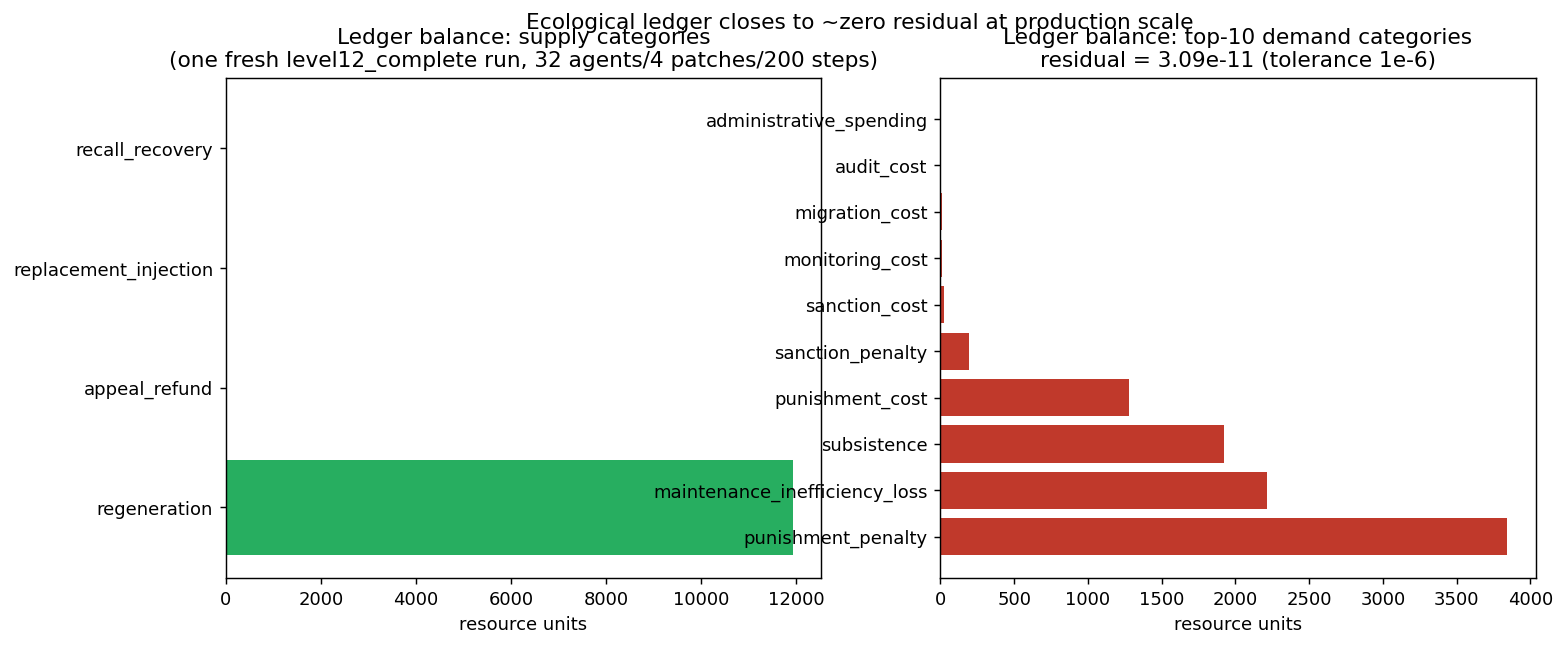
\includegraphics[width=0.95\textwidth]{figures/main/l12b_fig1_ledger_balance.png}
\caption{Level 1.2b ecological ledger: supply categories (left; dominated
by patch regeneration) and top-10 demand categories (right) for one fresh
diagnostic \texttt{level12\_complete} run. Residual $3.09\times10^{-11}$
against a documented tolerance of $10^{-6}$ on this run; across the full
576-run production design the maximum residual was $5.9\times10^{-9}$.}
\label{fig:l12b-ledger}
\end{figure}

\begin{figure}[htbp]
\centering
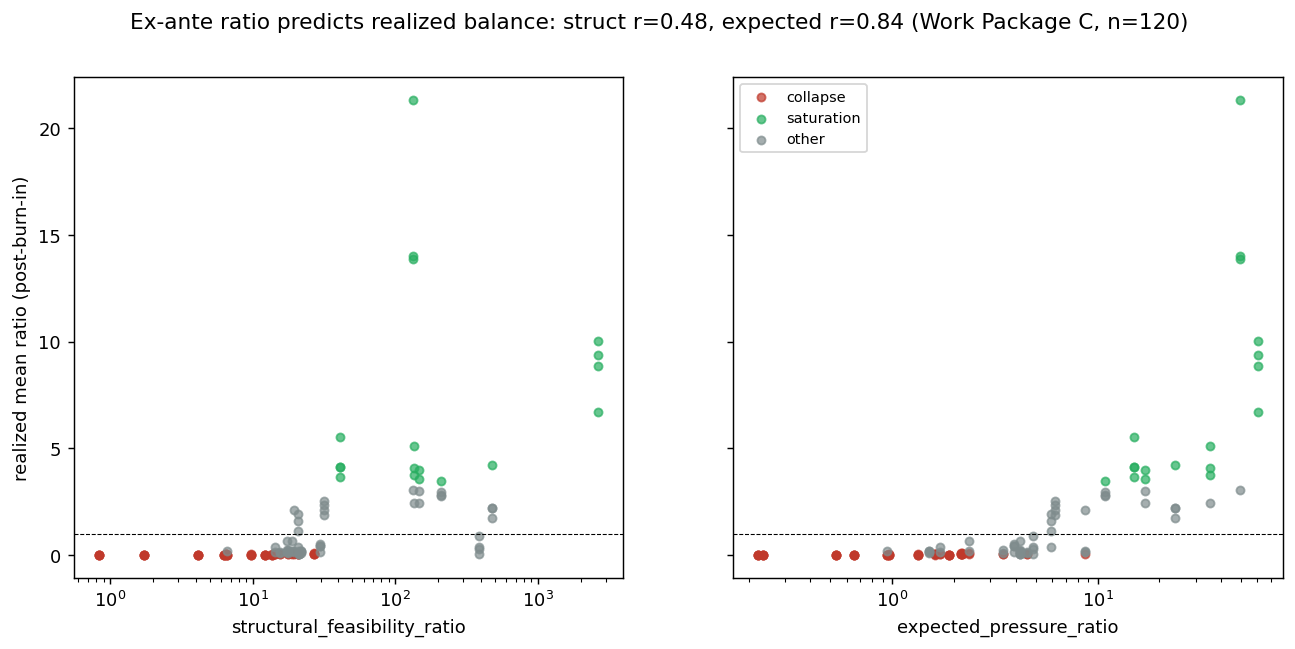
\includegraphics[width=0.75\textwidth]{figures/main/l12b_fig2_feasibility_ratios.png}
\caption{Ex-ante structural feasibility ratio and expected-pressure ratio
plotted against realized ecological balance ($n=120$ feasibility-map
runs). The expected-pressure ratio (Pearson $r\approx0.84$) tracks
realized balance substantially better than the structural ratio
($r\approx0.48$). Descriptive correlation, computed post hoc against
outcomes the ratios themselves never used for stratification.}
\label{fig:l12b-feasibility-ratios}
\end{figure}

\begin{figure}[htbp]
\centering
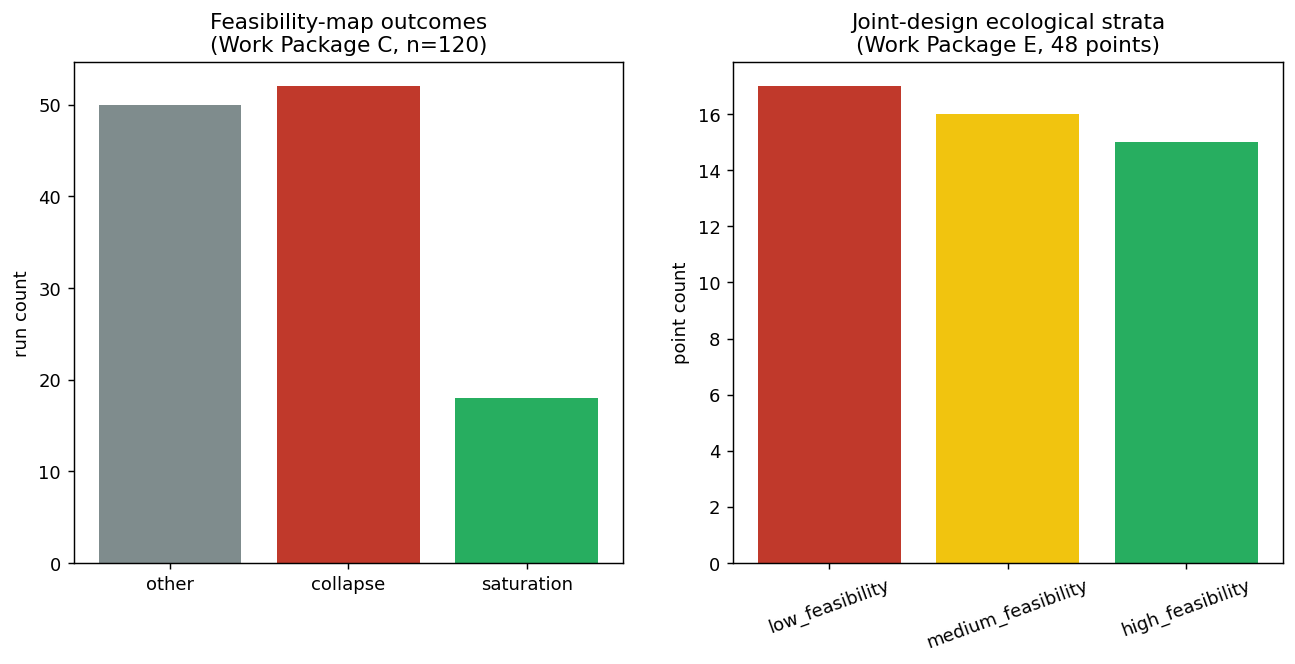
\includegraphics[width=0.85\textwidth]{figures/main/l12b_fig3_feasibility_strata.png}
\caption{Feasibility map and the tertile ecological strata (low/medium/
high expected-pressure ratio) frozen before the main joint discovery
design was generated.}
\label{fig:l12b-feasibility-strata}
\end{figure}

\begin{figure}[htbp]
\centering
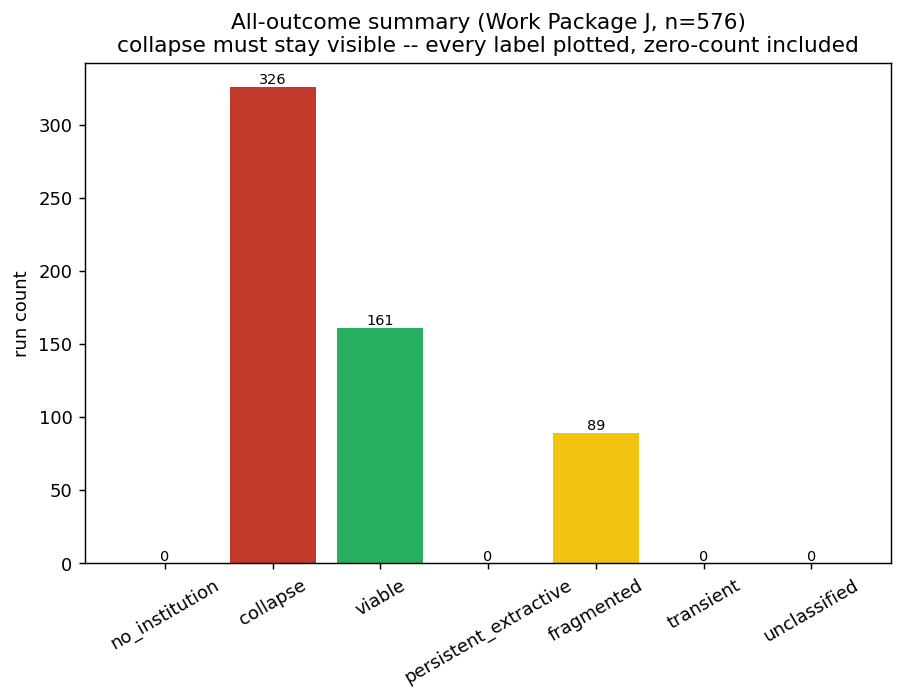
\includegraphics[width=0.75\textwidth]{figures/main/l12b_fig4_outcome_distribution.png}
\caption{Level 1.2b Work Package J complete all-outcome distribution
($n=576$), every label plotted including zero-count labels: collapse=326,
viable=161, fragmented=89, all others 0.}
\label{fig:l12b-outcome-distribution}
\end{figure}

\begin{figure}[htbp]
\centering
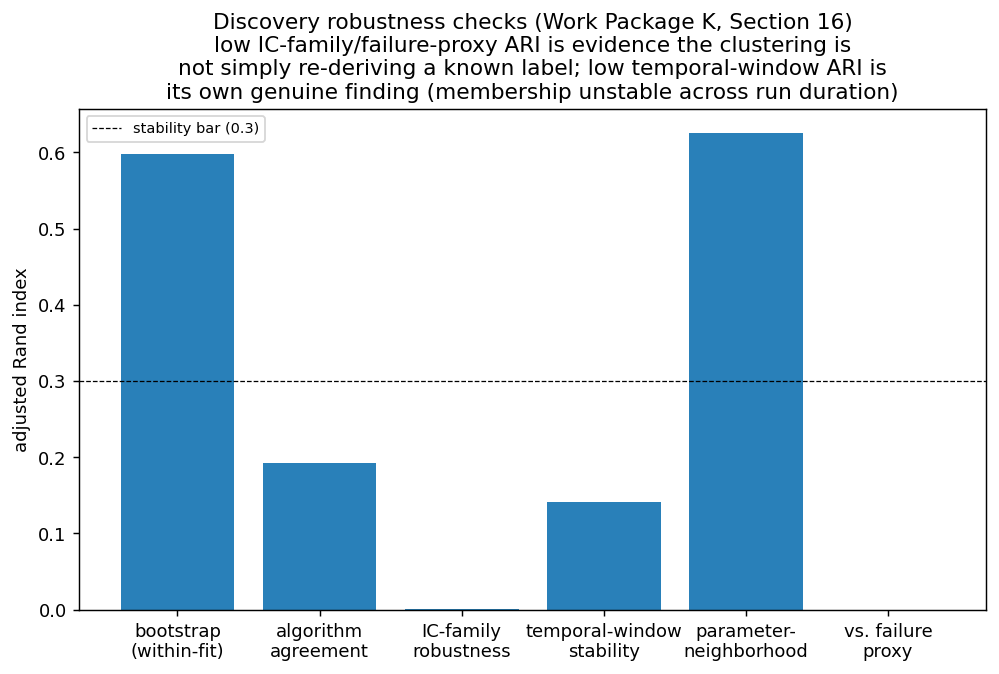
\includegraphics[width=0.85\textwidth]{figures/main/l12b_fig5_stability_metrics.png}
\caption{Level 1.2b discovery-pool clustering stability diagnostics:
bootstrap adjusted Rand index, pairwise algorithm-agreement adjusted Rand
index, missingness-strategy robustness, and temporal-window stability.
Descriptive fit diagnostics, not a causal claim.}
\label{fig:l12b-stability-metrics}
\end{figure}

\begin{figure}[htbp]
\centering
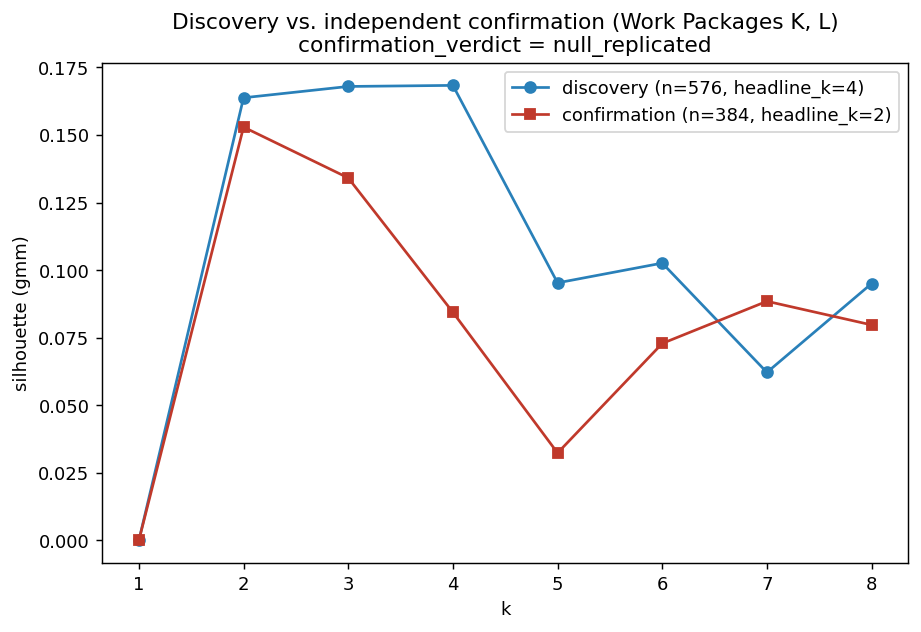
\includegraphics[width=0.75\textwidth]{figures/main/l12b_fig6_discovery_vs_confirmation.png}
\caption{Gaussian-mixture silhouette-by-$k$ curves: discovery pool
($n=576$, headline $k=4$) versus independent fresh confirmation pool
($n=384$, headline $k=2$), confirmation\_verdict=\texttt{null\_replicated}.
Descriptive null replication on disjoint data.}
\label{fig:l12b-discovery-confirmation}
\end{figure}

\begin{figure}[htbp]
\centering
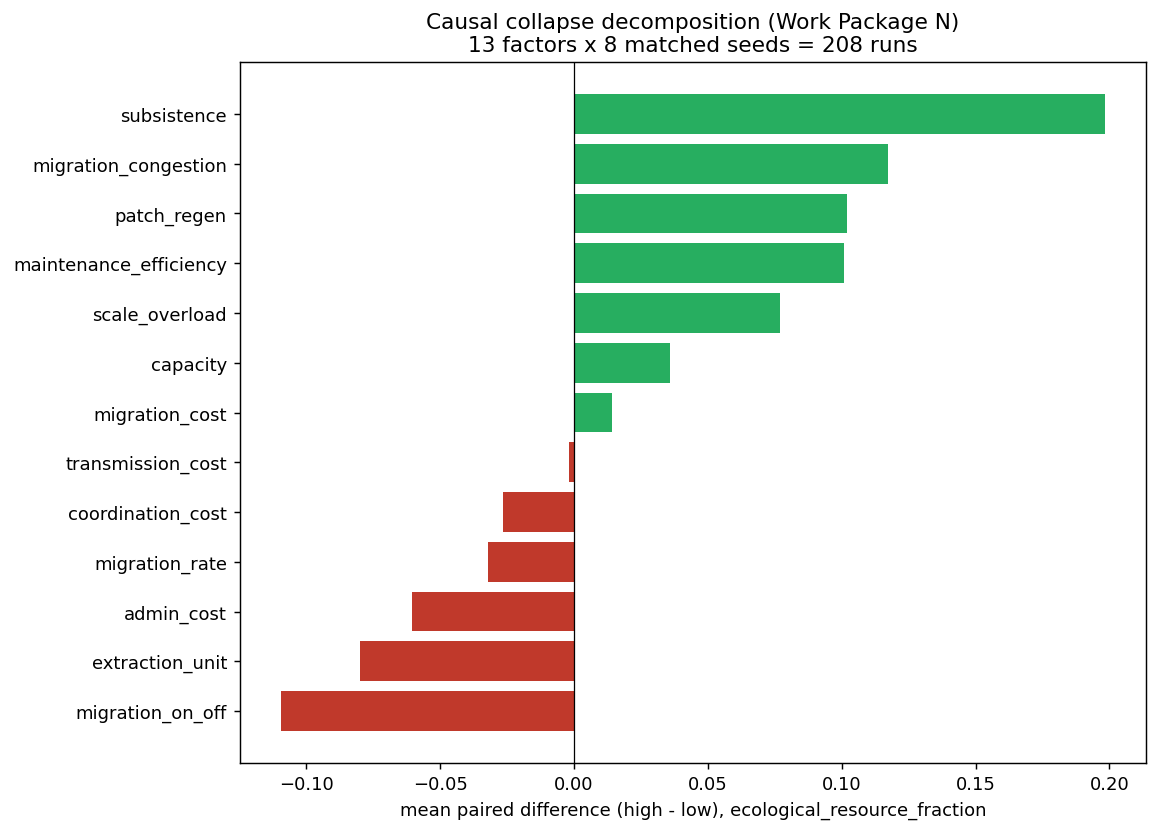
\includegraphics[width=0.9\textwidth]{figures/main/l12b_fig7_causal_ablation.png}
\caption{Work Package N thirteen-factor matched-seed causal-ablation
effect sizes on ecological-fraction outcomes ($n=208$ runs, 8 matched
pairs per factor). Causal evidence (matched-seed, \texttt{rng\_%
mode="mechanism\_substreams"}), distinct from every descriptive figure
above.}
\label{fig:l12b-causal-ablation}
\end{figure}

\subsection{Level 1.3 / Level 1.3b: the historically extended substrate}
\label{sec:results-l13}

\textbf{Historical effect on institutional response.} History causally and
persistently shapes institutional trajectories. Sham machinery validated
12/12 seeds byte-identical to control (Level 1.3b Stage 6); three of four
real history-erasure/reversal/equalization interventions produced real,
non-decaying, in several tests \textit{growing} final-sustained
divergence: \texttt{pressure\_memory\_only} 0.054, \texttt{entrenchment\_%
only} 0.072, \texttt{all\_history} 0.069 (mean $|S_{\text{obs}}|$ gap).
Level 1.3's own earlier, pooled-observational counterfactual (Stage 5:
erased-versus-base $\approx0.0027$, reversed-versus-base $\approx0.0116$)
pointed the same direction at smaller effect size, before purpose-designed
sham validation existed.

\textbf{Ordering effect: real but modest and direction-inconsistent.}
Level 1.3b Stage 3 (216 runs, purpose-designed factorial): 24.1\%
($S_{\text{obs}}$) and 32.4\% ($Z_{\text{obs}}$) of 108 matched pairwise
contrasts show a seed-clustered bootstrap CI excluding zero; direction is
consistent for one of three ordering-pair comparisons (27/36) and
inconsistent for the other two (20/36, 14/36). Level 1.3's own Stage 3 (72
runs, pooled design) found a comparable $\approx6$--$7.5\%$ relative
spread across six orderings.

\textbf{Discreteness, tested twice, rejected twice, more decisively the
second time.} Level 1.3's six-way verdict: \texttt{D\_continuum} (headline
$k{=}2$, silhouette 0.334, failed independent fresh-data reproduction:
log-likelihood $-1.29$ train versus $-6.05$ fresh). Level 1.3b's
eight-way verdict, from a purpose-designed pool and reusing Level 1.2b's
own frozen classifier unmodified: \texttt{D\_persistent\_continuum}
(headline $k{=}8$ by BIC, but silhouette never clears 0.15 across any
tested $k$, best $=0.143$ at $k{=}2$; cross-algorithm adjusted Rand index
0.016--0.357; cross-ecological-stratum adjusted Rand index $-0.043$ to
$-0.014$) (\cref{tab:l13-vs-l13b-discreteness}).

\textbf{$S_{\text{obs}}$--$Z_{\text{obs}}$ coupling: real, modest, and
weighting-sensitive.} Level 1.3 Stage 8 (pre-audit, $n=228$ pooled): Pearson
$r=0.888$, Spearman $\rho=0.913$. Level 1.3b Stage 9 (measurement-weighting
audit, $n=240$): equal-weight $r=0.264$, partial (controlling ecological
stratum) $r=0.272$, between-point $r=0.285$, within-point $r=0.261$,
leave-one-component-out range 0.175--0.307, PCA-weighted $r=0.136$ (a
genuine outlier, roughly half the equal-weight figure). Zero shared
component dimensions between the two composites, confirmed directly; PCA
does not cleanly recover an $S$/$Z$ axis split (PC1 loaded by both
legitimacy channels together).

\textbf{Bargaining activation, repaired and confirmed at scale.} 166/240
(69.2\%) Stage 4 runs activate under \texttt{repeated\_shocks} pressure;
20/24 (83\%) Stage 2 calibration cells land in the target range at
unmodified Level 1.1/1.2b defaults --- an observer-construction fix, not a
generative recalibration.

\begin{table}[htbp]
\centering
\caption{Discreteness testing, Level 1.3 versus Level 1.3b: both verdicts
reject discrete institutional families, reached via Level 1.2b's own
frozen classifier reused unmodified at both milestones.}
\label{tab:l13-vs-l13b-discreteness}
\adjustbox{max width=\textwidth}{\begin{tabular}{@{}llll@{}}
\toprule
\textbf{Metric} & \textbf{Level 1.3} & \textbf{Level 1.3b} & \textbf{Note} \\
\midrule
Design & pooled, post hoc (Stages 3--5) & purpose-designed (Stage 4) & 1.3b avoids 1.3's own confound \\
$n$ discovery pool & 216 & 240 & \\
Headline $k$ / selection rule & 2 (silhouette) & 8 (BIC) & different selection metrics led \\
Best silhouette (any $k$) & 0.334 ($k$=2) & 0.143 ($k$=2) & 1.3b never clears 0.15 floor \\
Bootstrap stability (mean ARI) & 0.917 & 0.752 & both clear 0.3 floor \\
Cross-algorithm agreement (ARI) & 0.291 (mean) & 0.016--0.357 (range, excl.\ non-independent pair) & both weak \\
Fresh-data reproduction & failed ($-1.29\to-6.05$ log-lik.) & mixed (+3.11 gap, but continuous candidate ties it) & \\
Cross-stratum reproduction & not tested & $-0.043$ to $-0.014$ (ARI) & 1.3b only; near-zero/negative \\
Formal verdict & \texttt{D\_continuum} & \texttt{D\_persistent\_continuum} & same top-level label, independent evidentiary path \\
\bottomrule
\end{tabular}
}
\end{table}

\begin{table}[htbp]
\centering
\caption{Level 1.3b Stage 6 sham-controlled history-erasure/reversal/
equalization intervention: mean $|S_{\text{obs}}|$ gap versus control by
window (12 matched seeds per arm).}
\label{tab:history-intervention}
\adjustbox{max width=\textwidth}{\begin{tabular}{@{}lrrrr@{}}
\toprule
\textbf{Arm} & \textbf{Early} & \textbf{Middle} & \textbf{Late} & \textbf{Final-sustained} \\
\midrule
\texttt{sham\_identical\_state\_copy} & \multicolumn{4}{c}{12/12 seeds byte-identical to control at every window} \\
\texttt{pressure\_memory\_only} & n/r & n/r & n/r & 0.054 \\
\texttt{entrenchment\_only} & 0.0 & 0.017 & 0.065 & 0.072 \\
\texttt{legitimacy\_history\_only} & n/r & 0.009 & n/r & $\approx4\times10^{-12}$ \\
\texttt{all\_history} & n/r & n/r & n/r & 0.069 \\
\bottomrule
\end{tabular}
}

\medskip
\noindent\footnotesize n/r = not individually reported at that window in
\texttt{docs/level1.3b\_scientific\_note.md}; the qualitative pattern
(middle-window gaps 0.009--0.017, growing to final-sustained 0.054--0.072
across the three non-legitimacy arms) is reported in aggregate even where
a specific arm's own middle/late value is not.
\normalsize
\end{table}

\section{Discussion}
\label{sec:discussion}

\subsection{A general governance-generative substrate}
\label{sec:disc-substrate}

Across ten development milestones, the model demonstrated generative
sufficiency at every layer it was asked to support: bilateral cooperation
and reciprocity produce measurable, heterogeneous cooperation dynamics; an
accounted ecology produces genuine regime diversity; locally shared rules,
proposed and adopted from local information alone, reproducibly form and
persist unforced; delegation, discretion, and accountability all activate,
interact, and are each independently detectable in the observer layer;
institutions can observe each other, transmit components, compete via
migration, and scale across jurisdictions; and, as of Level 1.3/1.3b,
historically structured pressure, entrenchment, and legitimacy accumulate
and causally shape institutional response, sham-validated against a
fork-machinery artifact. None of this required, at any point, encoding a
target macro-state, a governance label, or a trajectory count. This is the
sense in which we call the substrate \textit{generatively sufficient}: it
is capable of producing institutions, institutional variation, and now
historically conditioned institutional trajectories, as genuine emergent
consequences of micro-rules.

\subsection{Institutional emergence without discrete phenotype convergence}
\label{sec:disc-emergence-without-convergence}

What the discovery pipeline found, at every scale and in both the
synchronic and historical substrates, is that generative sufficiency does
not, by itself, imply \textit{phenotypic convergence} onto a small number
of recurring configurations. Level 1.2's null result was legitimately
ambiguous, because near-universal collapse could have been suppressing
institutional variation the discovery pipeline never got to see. Level
1.2b removed that ambiguity and the result strengthened rather than
changed in kind: a \texttt{continuum} verdict, independently replicated as
\texttt{null\_replicated} on fresh data. Level 1.3 then asked whether
adding history changes this answer, on pooled, exploratory evidence
leaning \texttt{continuum} again but resting on one post hoc pool. Level
1.3b asked the same question with a purpose-designed, preregistered,
causally instrumented program, and the answer sharpened rather than
softened: \texttt{D\_persistent\_continuum}, with a discreteness rule that
failed to clear even its own entry-level silhouette floor at any tested
$k$ --- a more decisive rejection of discrete structure than the
synchronic substrate itself produced. History is real and causally
demonstrated; discreteness is not.

\subsection{History is real, causal, and persistent --- without producing discrete families}
\label{sec:disc-history-real}

This is the paper's own central, and initially counter-intuitive,
finding, and it is worth stating plainly because it is easy to conflate
the two questions it separates. ``Does history matter?'' and ``does
history sort outcomes into discrete families?'' are different questions,
and Level 1.3b's evidence answers them differently. History matters:
Section~\ref{sec:level13b-h5h6}'s sham-validated intervention design ---
the strongest causal design this project has built --- shows that erasing,
reversing, or exposure-equalizing a run's own realized pressure history
produces a real, non-decaying, and in several tests \textit{growing}
divergence from that same run with its history intact, validated against a
control proven to introduce zero spurious divergence on its own. This is
not a correlational association between history-adjacent variables and
outcomes; it is a controlled comparison of a system against a version of
itself with a specific piece of its own past removed. History does not,
however, sort outcomes into discrete families: the same milestone's own
discreteness test, applied via the identical unmodified rule Level 1.2b
established for the synchronic substrate, rejects discreteness more
decisively than the synchronic case did. A system can be genuinely,
causally path-dependent --- shaped by, and persistently different because
of, its own specific history --- while the space of trajectories that
history can produce remains continuous rather than partitioned into a
small number of recurring types. Increasing-returns and lock-in dynamics
in the historical-institutionalist literature
(\cref{sec:historical-institutionalism}) are typically illustrated with
discrete case comparisons (this country locked in one path, that country
another), but nothing in that theoretical tradition actually requires the
space of possible paths to be discrete; a continuous space with strong,
persistent path dependence is equally consistent with it, and is what this
model's own evidence supports.

\subsection{The richer generative state and the triangulation logic}
\label{sec:disc-triangulation}
\label{sec:disc-richer-state}

Level 1.2/1.2b's own observer-only phenotype vector characterized a
synchronic configuration. Level 1.3/1.3b's own historical mechanisms make
explicit that the object worth tracking is richer: a governance
configuration together with the history that produced it. We formalize
this, at the level of the model's own generative state, as

\begin{equation}
\mathcal{G}_t = [S_t,\, Z_t,\, H_t,\, E_t,\, L_t,\, P_t,\, R_t,\, C_t,\, \ldots]
\label{eq:rich-state}
\end{equation}

where $S_t$ and $Z_t$ denote the model's own observer-side state-capacity-
and constraint-adjacent composites ($S_{\text{obs}}$, $Z_{\text{obs}}$,
\cref{sec:observer-metrics-l13}) at simulation time $t$; $H_t$ is
accumulated historical/pressure state (the specific realized sequence of
security, bargaining, and coordination-complexity pressure, not merely its
current level); $E_t$ is accumulated entrenchment; $L_t$ is the dual
performance/procedural legitimacy state; $P_t$ denotes the currently active
pressure levels themselves (as distinct from their accumulated history
$H_t$); $R_t$ denotes realized institutional structure (delegation,
monitoring, sanctioning configuration); and $C_t$ denotes coordination/
transmission state across jurisdictions. The ellipsis is deliberate: this
is not a claim that eight dimensions are exhaustive, only that $S_t$ and
$Z_t$ alone --- the dissertation's own two axes --- are not sufficient to
characterize a governance configuration once history is admitted as
causally consequential. $S$ and $Z$ remain the central, interpretively
load-bearing axes of this expanded state: they are what the dissertation's
own SEM analysis identifies from real survey data, and what this paper's
own $S_{\text{obs}}$/$Z_{\text{obs}}$ composites are built, independently,
to approximate. The other components of $\mathcal{G}_t$ do not replace $S$
and $Z$; they explain \textit{movement through} $S$/$Z$ space --- why a
given configuration sits where it does and how it is likely to move next
--- in a way a purely synchronic, two-dimensional snapshot cannot.
\Cref{tab:expanded-state} summarizes every symbol in $\mathcal{G}_t$
against its concrete model implementation.

\begin{table}[htbp]
\centering
\caption{The expanded generative state $\mathcal{G}_t$: symbol, denotation, and model implementation.}
\label{tab:expanded-state}
\adjustbox{max width=\textwidth}{\begin{tabular}{@{}lp{6.5cm}p{5.8cm}@{}}
\toprule
\textbf{Symbol} & \textbf{Denotes} & \textbf{Model implementation} \\
\midrule
$S_t$ & State-capacity-adjacent observer composite & $S_{\text{obs}}$: mean of delegation, administrative\_function, monitoring, interpatch\_coordination, performance\_legitimacy \\
$Z_t$ & Institutional-constraint-adjacent observer composite & $Z_{\text{obs}}$: mean of accountability, bargaining\_participation, procedural\_legitimacy \\
$H_t$ & Accumulated historical/pressure state (full realized sequence, not just current level) & Per-channel pressure history series (security, bargaining, coordination-complexity) \\
$E_t$ & Accumulated institutional entrenchment & Age-dependent amendment/dissolution-resistance index \\
$L_t$ & Dual legitimacy state & Independent performance ($L_P$) and procedural ($L_R$) ledgers \\
$P_t$ & Currently active pressure levels (as distinct from accumulated history $H_t$) & Instantaneous per-channel pressure value at step $t$ \\
$R_t$ & Realized institutional structure & Delegation/monitoring/sanctioning configuration \\
$C_t$ & Coordination/transmission state across jurisdictions & Interpatch coordination links, component transmission history \\
$\ldots$ & Deliberately open --- not claimed exhaustive & \\
\bottomrule
\end{tabular}
}
\end{table}

This motivates the paper's own triangulation logic, introduced in
\cref{sec:intro-triangulation} and developed fully here. Three lines of
evidence bear on the dissertation's own $G=f(S,Z)$ framework, each
answering a question the others structurally cannot. \textit{SEM
identification} (the dissertation's own contribution) establishes, from
real cross-sectional survey data, that a two-factor $S$/$Z$ space fits
better than a collapsed one-dimensional ranking, and that real countries'
measured positions are not uniformly distributed within it. \textit{ABM
generative sufficiency} (Level 1.2/1.2b, extended by Level 1.3/1.3b)
establishes that a microscopic mechanism set, encoding none of $S$, $Z$, or
any trajectory label, is sufficient to produce heterogeneous configurations
occupying an analogous space, and --- new to this paper --- that adding
historically structured pressure and sequencing to that mechanism set
produces further, causally real heterogeneity without collapsing to a
small number of forms. \textit{Historical causal experimentation} (Level
1.3b's own sham-validated intervention design, unique to the ABM and
structurally unavailable to cross-sectional survey analysis, since no
survey can rerun a country's own history with one piece of it removed)
establishes that history's effect on institutional trajectory is causal,
not merely associational, within the tested mechanism set. None of these
three lines of evidence duplicates the others, and none is sufficient
alone: SEM identification cannot speak to generative sufficiency or
causal mechanism; ABM generative sufficiency cannot speak to whether real
countries' own historical trajectories are in fact governed by the same
dynamics; and historical causal experimentation within a simulated model
cannot, by itself, establish that real-world governance history behaves
the same way. Read together, they support a specific, bounded claim,
stated in full in \cref{sec:disc-boundary-claims} below. \Cref{tab:method-triangulation}
lays out all four sources of evidence side by side, including the
dissertation's own qualitative interpretive step, against what each does
and does not establish.

\begin{table}[htbp]
\centering
\caption{Methodological triangulation: what each line of evidence
establishes, its design, and its own limits.}
\label{tab:method-triangulation}
\adjustbox{max width=\textwidth}{\begin{tabular}{@{}p{2.6cm}p{4.0cm}p{4.0cm}p{4.2cm}@{}}
\toprule
\textbf{Method} & \textbf{What it establishes} & \textbf{Design} & \textbf{What it cannot establish} \\
\midrule
SEM identification (dissertation) & A 2-factor $S$/$Z$ space fits real survey data better than a 1-D ranking; real countries occupy non-uniform positions in it & Cross-sectional SEM, WVS Wave 7, real national cases & Generative sufficiency; causal mechanism; historical trajectory; discreteness of any typology laid over the space \\
ABM generative sufficiency (Level 1.2/1.2b, extended 1.3/1.3b) & A microscopic mechanism set, encoding none of $S$/$Z$/labels, is sufficient to produce heterogeneous configurations in an analogous space & Outcome-blind discovery, preregistered, independently replicated on fresh data & Whether real countries' own history follows the same dynamics; validation of the dissertation's specific empirical positions \\
Historical causal experimentation (Level 1.3b) & History's effect on simulated institutional trajectory is causal, not merely associational & Sham-controlled matched-seed intervention (state-copy control proven zero-divergence) & Whether real-world governance history behaves the same way; external validity beyond the tested mechanism set \\
Qualitative interpretation (dissertation \S4.4, this paper \S\ref{sec:disc-relationship-to-dissertation}) & A coherent narrative linking the two-dimensional space to named historical/institutional archetypes & Theorized typology over an identified coordinate space, not a cluster analysis & A statistical claim of discreteness; the dissertation's own text is explicit on this point (\cref{sec:intro-synchronic-to-historical}) \\
\bottomrule
\end{tabular}
}
\end{table}

\subsection{Continuum versus typology, restated for the historical substrate}
\label{sec:disc-continuum-vs-typology}

The methodological point from \cref{sec:why-null-informative} applies with
undiminished force to Level 1.3b's own eight-way result: silhouette-based
model selection alone cannot distinguish a genuine discrete structure from
a single dominant bisection of a smooth continuum, and a Bayesian
information criterion that is still falling at the edge of a tested range
is a signature of a still-improving flexible density fit, not evidence of
a converged discrete-family count. Level 1.3b's own BIC curve
(\cref{fig:l13b-bic}) falls sharply and without turning upward all the way
to $k{=}8$, the edge of the tested range --- precisely the pattern that
should raise, not settle, the question of whether a wider search would
find an even lower BIC at $k{=}9$ or beyond, which is exactly why this
paper does not report BIC in isolation anywhere and why
\cref{fig:l13b-bic} is captioned, and paired, with the weak cross-algorithm
and cross-stratum agreement evidence that argues directly against reading
$k{=}8$ as eight genuine institutional species (\cref{sec:disc-boundary-claims}).

\subsection{Relationship to the dissertation's S--Z trajectories}
\label{sec:disc-relationship-to-dissertation}

We can now state this relationship more precisely than Level 1.2b's own
discussion could, because Level 1.3b adds evidence the earlier milestone
did not have. The dissertation's SEM result is a statement about the joint
distribution of measured confidence and constraint variables across a
fixed set of existing national cases, at one historical moment, aggregated
at the level of already-formed states; its own text is explicit that this
identifies a coordinate space and does not classify countries or predict
trajectories, and that the three named trajectories are a qualitative,
theorized typology laid over that space, not a statistically discovered
partition (\cref{sec:intro-synchronic-to-historical}). This paper's own
ABM results, across all four milestones, are statements about what a
general microscopic mechanism set --- with and without historically
structured pressure --- can generate from scratch, blind to any expected
answer. Four specific things follow from combining them, stated precisely
to track exactly what was and was not tested.

First, the ABM's own generative substrate is sufficient to produce
heterogeneous governance configurations occupying a space with axes
plausibly analogous to $S$ and $Z$ (Levels 1.2/1.2b), and the observer-side
composites built for those axes do show a real, if modest and
weighting-sensitive, positive coupling (Level 1.3b Stage 9,
$r\approx0.26$--$0.29$ across defensible variants) --- weak, indirect
corroboration that state-capacity-like and constraint-like dimensions of a
generated governance space are related rather than orthogonal, consistent
with, though not a statistical test of, the dissertation's own finding
that $S$ and $Z$ are correlated but distinct factors. Second, historically
structured pressure and sequencing causally and persistently shape where a
simulated jurisdiction sits and how it got there (Level 1.3b Stage 6) ---
direct generative support for treating governance trajectories as
path-dependent processes, not merely static positions, which is exactly
the temporal dimension the dissertation's own SEM analysis is explicit
that it cannot supply (\cref{sec:historical-institutionalism}). Third,
neither the synchronic nor the historically extended substrate compresses
its own outcome space into three, or any other small fixed number of,
discrete, well-separated forms --- a null result about \textit{this
model's own generated space}, not a claim about whether real countries'
governance configurations are or are not discretely clustered, which this
paper's own ABM evidence cannot settle either way (\cref{sec:limitations}).
Fourth, and precisely because of the third point, the dissertation's own
three trajectories remain a legitimate, unaffected empirical finding at
their own analytical level: they are qualitative regions the dissertation
itself never claimed were statistically discrete, and this paper's own
result --- that a generative model producing an analogous space finds that
space continuous rather than discretely partitioned, even once
historically structured path dependence is added --- is consistent with,
and arguably strengthens the interpretive case for, reading the three
trajectories as coarse-grained, historically and institutionally
interpreted \textit{regions} of a continuous space rather than as discrete
natural kinds, which is a reading the dissertation's own methodology
(a two-dimensional coordinate space plus a qualitative typology, not a
cluster analysis) is already consistent with.

\subsection{What this paper does not claim: boundary conditions}
\label{sec:disc-boundary-claims}

Precisely because the evidence above is easy to overstate, we state five
specific boundary conditions explicitly, each ruling out a claim this
paper's own results could be mistaken for but do not support.

\textit{A statistical component count is not a species count.} Level
1.3b's leading discrete candidate has the lowest BIC at $k{=}8$ components;
this is a property of a specific model-selection criterion applied to a
specific finite sample, not a discovery of eight institutional species.
No tested $k$ clears even the classifier's own entry-level silhouette
floor (\cref{sec:level13b-h7h8}).

\textit{Statistical components are not recurrent institutional phenotypes.}
A recurrent phenotype, in this project's own vocabulary
(\cref{sec:terminology-discipline}), additionally requires passing
preregistered cross-seed, cross-algorithm, and bootstrap-stability
criteria; Level 1.3b's own $k{=}8$ candidate fails cross-algorithm
agreement (0.016--0.357 once the non-independent pair is excluded) and
cross-ecological-stratum reproduction ($-0.043$ to $-0.014$).

\textit{Recurrent phenotypes, had they been found, would not automatically
be dynamical attractors.} No claim anywhere in this paper asserts that any
discovered structure, at any milestone, is a state the system returns to
after perturbation; that specific, stronger claim requires direct evidence
of majority recovery on every tracked dimension
(\cref{sec:level12b-scale-causal}), which this project has never found for
any candidate structure at any milestone.

\textit{A multi-component model beating a single-Gaussian null is not
evidence of eight, or any specific number of, discrete families.} Level
1.3b's own Stage 8 fresh-data comparison shows the leading $k{=}8$
candidate beats a $k{=}1$ null on fresh data (\cref{sec:level13b-h7h8}) ---
but the leading \textit{continuous} candidate beats the same null by a
comparable margin, and an information criterion that has not converged
within the tested range cannot, on its own, license treating $k{=}8$ as
the true count rather than an artifact of where the search stopped.

\textit{Weak cross-algorithm and cross-stratum agreement rules out
treating any current partition as a discrete-family finding.} This is not
a subtle qualification; it is the single most decisive piece of evidence
in Level 1.3b's own record, and it is why every figure and table in this
paper reporting the $k{=}8$ result is paired with the cross-algorithm and
cross-stratum evidence that contextualizes it
(\cref{fig:l13b-bic,fig:l13b-discreteness}), never presented alone.

We add, finally, a fifth and more general boundary condition specific to
this paper's own claim structure: nowhere in this paper does a simulation
result from the ABM constitute empirical validation of the dissertation's
own three trajectories, of the exact number of governance archetypes real
countries occupy, or of the specific $S$/$Z$ values at which real countries
sit. The ABM's own $S_{\text{obs}}$/$Z_{\text{obs}}$ composites are
independently constructed, observer-side quantities, never fit to or
validated against the dissertation's own survey-derived latent factors;
any correspondence between them is, at most, weak structural corroboration
of the dissertation's own two-axis framing, not a validation of its
specific empirical content.

\subsection{Historical sequencing: confirmed as real, not merely motivated}
\label{sec:disc-historical-sequencing}

Level 1.2b's own discussion motivated, but explicitly did not test, a
formal decomposition $M_{\text{historical}} = M_{\text{general}} + H$. This
paper's second half tests it directly, and $H$ is no longer merely a
hypothesis: Level 1.3/1.3b implement $H$ as three pressure-transmission
channels, institutional entrenchment, and dual legitimacy ledgers, and
Level 1.3b's own sham-validated causal intervention design shows that $H$,
so implemented, causally and persistently shapes institutional response.
We restate \cref{eq:historical-decomposition-intro} with this paper's own
evidentiary status made explicit:

\begin{equation}
M_{\text{historical}} = M_{\text{general}} + H, \qquad
G_t = f\bigl(S_t, Z_t;\; H_{0:t},\, E_t,\, L_t,\, P_t,\, \ldots\bigr)
\label{eq:historical-decomposition-tested}
\end{equation}

where the macro-level right-hand side makes explicit that governance
outcome at time $t$ depends not only on current-state $S_t$, $Z_t$ but on
the full realized history $H_{0:t}$, accumulated entrenchment $E_t$,
legitimacy state $L_t$, and current pressure $P_t$ --- exactly the
dependency structure $\mathcal{G}_t$ (\cref{eq:rich-state}) is built to
track. What remains genuinely untested, and what this paper does not
claim, is whether $H$ as implemented here corresponds to the specific
historical mechanisms (critical junctures, colonial extraction, war-driven
state-building) the historical-institutionalist literature identifies in
real cases, whether the model's own parameter domain and duration are
representative of real historical timescales, and whether real governance
systems' own historical processes are governed by dynamics of the same
qualitative shape this model's tested mechanism set produces. Explaining
why real governance systems concentrate around particular recurring
trajectories --- as opposed to why a generative model of the kind built
here does or does not --- is deferred to future, historically calibrated
research (\cref{sec:limitations}).

\section{Limitations}
\label{sec:limitations}

\begin{table}[htbp]
\centering
\caption{Summary of model and evidentiary limitations.}
\label{tab:limitations}
\adjustbox{max width=\textwidth}{\begin{tabular}{@{}p{0.32\textwidth}p{0.63\textwidth}@{}}
\toprule
\textbf{Limitation} & \textbf{Scope / disclosed status} \\
\midrule
Parameter domain \& duration & Results conditional on tested mechanism set, parameter ranges, and run length ($\le$700 steps); not a claim about untested regions. \\
Collapse still modal & 56.6\%--78.1\% collapse across L1.2b pooled samples even after stratification; non-collapse variation is the minority of the sampled space. \\
\texttt{shared\_lineage\_persistence} unevaluated & Would require a 4th 576-run re-simulation with per-run lineage export; judged low-value given the continuum/null-replication result; disclosed, not filled here. \\
Temporal-representation validation subset & 4 burn-in definitions validated on 12 of 576 discovery runs, for compute-budget reasons stated in advance. \\
Supplementary significance tests & L1.2 Section 13 Wilcoxon tests ($n$=8 pairs) are supplementary; L1.2b's 13-factor decomposition reports effect sizes, not significance tests, by design. \\
Reconstructed audit text & Verbatim governing-specification text for two completion-report sections was unrecoverable after a mid-milestone context compaction; this paper reports the reconstructed audit, disclosed as such. \\
Single implementation & All results from one model lineage, one research team; independent re-implementation would strengthen confidence the continuum finding is not implementation-specific. \\
No historical-sequencing test & $H$ in $M_{\text{historical}}=M_{\text{general}}+H$ is not implemented or tested anywhere in this paper; it is a motivated hypothesis for future work only. \\
\bottomrule
\end{tabular}
}
\end{table}

\textbf{Parameter domain and duration.} Every result in this paper is
conditional on the tested mechanism set, the tested parameter domain, and
the tested run durations (up to 700 steps at Level 1.2b's production
scale). A \texttt{continuum} verdict is a statement about the outcome
space actually sampled; it is not a proof that no parameter region or
longer duration exists in which discrete institutional clustering would
emerge. \cref{sec:appendix-tables} reports the full sampled ranges.

\textbf{Collapse remains the modal outcome.} Even at Level 1.2b's much
larger and ecologically stratified scale, collapse remained the single
largest outcome class in every pooled sample (56.6\%--78.1\% depending on
the sample). Non-collapse institutional variation, while far more
plentiful than at Level 1.2 (161 viable and 89 fragmented runs out of 576
at discovery, versus 2 non-collapse runs out of 24 at Level 1.2), is still
a minority of the sampled space; a design deliberately oversampling the
non-collapse region --- informed by, but going beyond, the causal
ablation's own findings about subsistence cost and migration --- would
give any future discovery attempt more institutional variation to work
with, at the cost of no longer representing the model's own unconditional
outcome distribution.

\textbf{Evidence gaps disclosed, not filled.} \texttt{shared\_lineage\_%
persistence}, one of six candidate explanations Work Package O considered
for cross-run phenotype similarity, was never evaluated; doing so would
require a fourth full 576-run re-simulation with per-run lineage
identifiers exported, which the source project judged low-value given
that the continuum and null-replication findings already independently
established that no discrete candidate structure exists for shared
ancestry to explain. We report this as an open evidence gap rather than
filling it by rerunning simulations for this paper, per this paper's own
task discipline of not rerunning expensive computation merely to
strengthen a narrative.

\textbf{Temporal-representation validation subset.} Level 1.2b's four
burn-in-sensitivity definitions and window-bounds machinery were validated
on a disclosed 12-seed-run subset of the main design, not the full 576-run
pool, for compute-budget reasons stated at the time rather than after
seeing results.

\textbf{Supplementary statistical tests.} The causal-ablation Wilcoxon
$p$-values reported in \cref{sec:level12-collapse} (Level 1.2, $n=8$
matched pairs per test) are explicitly supplementary, not confirmatory ---
too small a sample for a standalone significance claim on their own, and
reported as such rather than overclaimed. Level 1.2b's 13-factor
decomposition (\cref{sec:level12b-scale-causal}) reports effect sizes and
outcome-label transition counts rather than significance tests, by design.

\textbf{Reconstructed audit sections.} Two portions of Level 1.2b's own
completion documentation --- the exact verbatim text of its governing
specification's stop-condition and final-report sections --- were not
recoverable from that project's own session context after a mid-milestone
context compaction, and its own completion report discloses this
explicitly rather than fabricating numbered items to match a remembered
count. This paper reports the reconstructed audit the source project
performed in its place, not a verbatim reproduction of text that no
longer exists.

\textbf{Single research team, single model lineage.} Every result in this
paper comes from one model implementation, developed and audited by one
project, however extensively internally cross-checked (structural
firewalls, byte-for-byte no-op regression tests, independent ledger
verification, disjoint confirmation samples). External replication in an
independently implemented ABM sharing the same generative assumptions
would strengthen confidence that the continuum finding reflects the
mechanism set itself rather than an implementation-specific artifact, in
the spirit of the broader empirical-validation standards recommended for
agent-based modeling generally \parencite{windrum2007empirical}.

\textbf{Historical-sequencing test now performed, with its own disclosed
scope.} Unlike the Level 1.2/1.2b manuscript this paper revises, $H$ is now
implemented and tested (\cref{sec:level13,sec:level13b}). Its own scope is
bounded: Stage 5's persistence diagnostics and Stage 6's history-erasure
interventions both operate at one representative cell
(\texttt{entrenchment=moderate}, \texttt{legitimacy=dual},
\texttt{stratum=medium\_feasibility}), not the full Stage 3 factorial;
Stage 6's own causal design manipulates historical state (pressure memory,
entrenchment age, legitimacy scores) rather than testing every conceivable
historical intervention; and every Level 1.3b stage ran at a disclosed,
session-budget-scaled \textit{minimum} sample size (Stage 4: 240 of a
preferred 432--768; Stage 8: 96 of a preferred 144--288), not adjusted
after seeing results.

\textbf{Discrete-versus-continuous comparison uses non-commensurable
metrics.} Level 1.3b's own Stage 8 compares the leading discrete candidate
(log-likelihood) against the leading continuous candidate (reconstruction
error) on fresh data --- two metrics not on a common scale
(\cref{sec:level13b-h7h8}), one of the decision gate's own four concrete
``what would change this verdict'' items (extending the tested $k$ range
past 8; building a common discrete/continuous fresh-data metric; extending
Stage 5/6 to the full Stage 3 factorial; building a genuine multi-condition
cluster-assignment-stability diagnostic for H3).

\textbf{$S_{\text{obs}}$/$Z_{\text{obs}}$ are not the dissertation's SEM
latent factors.} Every claim in \cref{sec:disc-relationship-to-dissertation}
treating the ABM's own observer-side composites as weak corroboration of
the dissertation's $S$/$Z$ framework is explicitly bounded to that weak
sense; $S_{\text{obs}}$/$Z_{\text{obs}}$ were never fit to, validated
against, or constructed with reference to the dissertation's own survey
data or SEM output, and the dissertation itself reports no single $S$--$Z$
correlation coefficient for this paper to compare against in the first
place (\cref{sec:appendix-ledger}).

\textbf{Reconstructed governing specifications.} Both Level 1.3 and Level
1.3b's own governing specifications were authored at length in an earlier
working session whose exact verbatim text became unrecoverable after a
later context compaction; every downstream document (preregistration
modules, scientific notes, decision-gate reports) discloses this
explicitly rather than presenting a reconstructed hypothesis list as a
verbatim transcription, and this paper reports the reconstructed
hypotheses and findings the source project itself worked from
(\cref{sec:reproducibility}).

\textbf{Real governance systems, not simulated ones, remain untested.}
Every claim in this paper about historical path dependence, causal
divergence, and continuous versus discrete structure is a claim about
\textit{this generative model's own outcome space}, under the specific
mechanism set, parameter domain, and duration tested. Whether real
governance systems' own historical trajectories are governed by dynamics
of the same qualitative shape --- and, in particular, why real systems
appear to concentrate around a small number of recurring configurations,
if the dissertation's own three-trajectory reading is correct --- is not
addressed by any simulation result in this paper and is deferred to
future, historically calibrated research (\cref{sec:disc-historical-sequencing}).

\Cref{tab:conclusion-boundary} states, for every major claim in this
paper, whether it is supported, partially supported, unsupported, or
reserved for future work, as a single strict reference table.

\begin{table}[htbp]
\centering
\caption{Strict conclusion-boundary table: every major claim in this
paper, classified by evidentiary status.}
\label{tab:conclusion-boundary}
\adjustbox{max width=\textwidth}{\begin{tabular}{@{}p{6.2cm}p{2.4cm}p{6.2cm}@{}}
\toprule
\textbf{Claim} & \textbf{Status} & \textbf{Basis / what would change it} \\
\midrule
Atomic mechanisms are generatively sufficient to produce institutions and heterogeneous institutional outcomes & Supported & Levels 1.0--1.2b; unforced formation at every tested ecological candidate \\
Synchronic substrate does not compress outcomes into discrete recurring forms & Supported & Level 1.2/1.2b: continuum, independently replicated (null\_replicated) \\
Historically structured pressure/sequencing causally shapes institutional trajectory & Supported & Level 1.3b Stage 6: sham-validated, 3/4 real interventions show growing divergence \\
Historically extended substrate compresses outcomes into discrete recurring forms & Unsupported & Level 1.3b: silhouette never clears 0.15; weak cross-algorithm/cross-stratum agreement \\
Pressure-onset ordering produces a real effect & Partially supported & Real but modest, direction-inconsistent across ordering pairs (H2) \\
Entrenchment moderates persistence as a graded dose-response & Unsupported (as stated) & Mechanism works; composite effect non-monotonic (H4) \\
$S_{\text{obs}}$--$Z_{\text{obs}}$ are coupled & Supported, modest & $r\approx0.26$--$0.29$ across variants; not the same construct; PCA-weighted variant $r\approx0.14$ \\
ABM results validate the dissertation's 3 empirical trajectories & Unsupported --- not attempted & Different analytical levels; ABM cannot confirm/refute a cross-sectional SEM typology \\
Real governance systems are discretely speciated into 3 (or any fixed count of) trajectories & Out of scope & Requires historically calibrated real-world data, not simulation \\
$\mathcal{G}_t$ richer-state formalism improves on $S$/$Z$ alone for tracking simulated trajectories & Supported, within this model & Motivated by Level 1.3/1.3b's own findings; not independently validated against external data \\
Why real systems concentrate around specific recurring trajectories & Deferred & Future, historically calibrated research (\cref{sec:disc-historical-sequencing}) \\
\bottomrule
\end{tabular}
}
\end{table}

\section{Conclusion}
\label{sec:conclusion}

We built a general, microscopic, governance-generative agent-based model
from elementary mechanisms addressing cooperation, ecological viability,
information, enforcement, delegation, accountability, mobility, and
interpatch coordination, and, across four linked milestones, searched its
outcome space, blind to any expected answer, for recurrent institutional
phenotypes and for the causal role of history in producing them. The
synchronic substrate (Level 1.2/1.2b) is generatively sufficient ---
producing institutions and heterogeneous institutional outcomes from
purely local rules --- but not, by itself, sufficient to compress those
outcomes into a small number of discrete, well-separated forms; both a
24-run and a 576-run/384-run independently replicated search returned a
\texttt{continuum} verdict. Extending that substrate with historically
structured pressure, sequencing, entrenchment, and legitimacy (Level
1.3/1.3b) did not change this qualitative picture, but it did add
something the synchronic substrate could not: direct, sham-validated
causal evidence that history matters. Erasing, reversing, or
exposure-equalizing a simulated jurisdiction's own realized pressure
history produces a real, persistent, non-decaying divergence from that
same jurisdiction with its history intact, validated against a control
proven to introduce zero spurious divergence on its own --- the strongest
causal evidence for path dependence this project has produced. At the same
time, a purpose-designed, preregistered discreteness test, reusing the
synchronic substrate's own frozen classification rule unmodified, rejected
discrete institutional families more decisively for the historically
extended substrate than for the synchronic one: no tested cluster count
cleared even an entry-level silhouette floor, cross-algorithm agreement was
weak, and the leading partition did not reproduce across ecological
strata. History, in this model, is a real, causal, persistent conditioning
operator on where a governance configuration sits and how it got there ---
without collapsing the space of configurations into a fixed small number
of discrete attractors.

We have argued throughout that these two findings are not in tension. The
dissertation's own $S$/$Z$ coordinate space remains the central,
interpretively load-bearing frame for this paper's own results: the
model's independently constructed $S_{\text{obs}}$/$Z_{\text{obs}}$
composites show a real, if modest and weighting-sensitive, positive
coupling, weakly corroborating the dissertation's own finding that state
capacity and institutional constraint are related but distinct dimensions
of governance. What the historically extended substrate adds is not a
third discrete axis but a richer account of movement through that same
$S$/$Z$ space --- accumulated pressure history, entrenchment, and
legitimacy that jointly explain why a configuration sits where it does and
how it is likely to move next, formalized here as
$\mathcal{G}_t=[S_t,Z_t,H_t,E_t,L_t,P_t,R_t,C_t,\ldots]$ and
$G_t=f(S_t,Z_t;H_{0:t},E_t,L_t,P_t,\ldots)$. Three complementary lines of
evidence triangulate toward this account without duplicating one another:
the dissertation's own SEM identification of a two-dimensional coordinate
space from real survey data; this project's demonstration that a
microscopic mechanism set, encoding none of the dissertation's own
variables or labels, is generatively sufficient to populate an analogous
space and to move heterogeneously within it under historical pressure; and
a sham-validated causal intervention design, structurally unavailable to
cross-sectional survey analysis, showing that history's effect on
simulated institutional trajectory is causal rather than merely
associational. None of these three lines is sufficient on its own, and we
have been correspondingly careful, throughout this paper's own
terminological discipline, not to let a statistical component count stand
in for a species count, a recurrent phenotype for a dynamical attractor,
or a positive generalization gap against a weak null for genuine
discreteness.

The dissertation's three empirically observed governance trajectories
remain a legitimate, unaffected empirical finding at their own analytical
level, and this paper's own results neither confirm nor refute them
directly. What this paper's evidence does support is a specific,
bounded reading: those three trajectories are best understood as
historically and institutionally interpreted regions of a continuous,
path-dependent configuration space, rather than as discrete natural kinds
that a sufficiently powerful clustering algorithm would eventually recover
--- a reading the dissertation's own methodology, a coordinate space plus a
qualitative typology rather than a cluster analysis, is already consistent
with, and one this project's own generative and historical mechanisms are
jointly sufficient, though not yet calibrated to real historical data, to
produce and causally probe. Explaining why real governance systems
concentrate around particular recurring trajectories is deferred to future
historically calibrated research.

\section{Reproducibility and Data Availability}
\label{sec:reproducibility}

\textbf{Source model repository.} The generative model, observer layer,
experiment scripts, and every raw output artifact reported in this paper
are drawn from a private, version-controlled model repository
(\texttt{abm\_governance}, internal milestone label
\texttt{abm\_governance\_level1.0}), which this paper's own workspace
treats as read-only and does not modify, rename, delete, or regenerate.
Full model documentation lives in that repository's own
\texttt{docs/odd\_level0.1.md} through \texttt{docs/odd\_level1.3\_%
addendum.md} (ODD-style model description, extended additively at every
milestone), \texttt{docs/config\_reference.md} (every configuration
field), and \texttt{docs/level0.2\_scientific\_note.md} through
\texttt{docs/level1.3b\_scientific\_note.md} (per-milestone findings).
\texttt{dev\_mem/project\_vision.md} documents the generative/observer
separation and development philosophy this paper's
\cref{sec:model-genealogy,sec:model-methods} summarize;
\texttt{dev\_mem/status\_update.md} is that project's own chronological
development log.

\textbf{Determinism.} Every stochastic draw in the source model passes
through one explicit, seeded random-number generator per run; two runs
with the same configuration, including seed, are bit-for-bit identical.
Every causal (matched-seed) experiment at every milestone uses the
per-mechanism random-number substream architecture
(\texttt{rng\_mode="mechanism\_substreams"}), so that a paired comparison
isolating one mechanism never couples that mechanism's own random draws to
any other mechanism's draws under the nominal seed. Level 1.3b's own Stage
0 additionally found and fixed a cross-process frozenset-hash
non-determinism (\texttt{rules/transmission.py}, introduced at Level 1.2,
invisible to every prior single-process check) --- sorting the underlying
component-name union before tupling restored bit-for-bit determinism
across separate process launches of the same seed and configuration,
confirmed by a standing regression test
(\texttt{tests/test\_level13b\_cross\_process\_reproducibility.py}).

\textbf{Preregistration.} All four milestones freeze a hashed manifest
before generating data: Level 1.2's Stage 0 manifest
(\texttt{outputs/level12\_stage0\_preregistration/manifest.json}); Level
1.2b's Work Package I manifest
(\texttt{outputs/level12b\_stage\_i\_preregistration\_manifest/manifest.json},
SHA-256 \texttt{f5bd19df\ldots}); Level 1.3's own Stage 0 manifest; and
Level 1.3b's own manifest (\texttt{docs/level13b\_preregistration.md} ---
disclosed by its own source project as using the \texttt{level13b\_}
no-dot naming convention, an inconsistency introduced when the file was
first written and left as-is rather than renamed mid-milestone, since
other files already reference the existing path). Every downstream stage
script recomputes and verifies its own milestone's manifest hash before
proceeding, via \texttt{load\_and\_verify\_manifest()}, and Level 1.3b's
own manifest additionally freezes the eight-label decision-gate vocabulary
(\cref{sec:decision-gate-extended}) and an explicit note that its own
discovery pipeline's default must not be biased toward
\texttt{three\_families}.

\textbf{Software and testing.} The source model's test suite stood at
1,084 passed / 6 skipped / 0 failed / 0 warnings at the close of Level 1.2;
1,475 passed / 6 skipped / 0 failed / 0 warnings at the close of Level
1.2b (389 new tests); and 1,869 passed / 6 skipped / 0 failed / 0 warnings
immediately before Level 1.3b began (Level 1.3b's own disclosed preflight
baseline, identical to Level 1.3's own closing count). At the close of
Level 1.3b: \textbf{2,047 passed / 6 skipped / 0 failed / 0 warnings} (178
new tests across 19 files, exactly matching the delta from the 1,869
preflight baseline), run under \texttt{python -m pytest -q -W error -p
no:cacheprovider}, re-run in full as Level 1.3b's own closing verification
step rather than inferred from per-task runs. A whole-package,
non-fixed-module-list forbidden-terminology scan and a dedicated
SEM-firewall audit (which also confirms no dissertation-derived data file
exists anywhere in the repository) both passed throughout all four
milestones; Level 1.3b's own extension
(\texttt{tests/test\_level13b\_sem\_firewall\_extension.py}) adds a
docs-directory scan for \texttt{docs/level1.3b\_*.md} and reuses Level
1.3's own forbidden-term list unmodified, introducing no new forbidden
vocabulary. No milestone's generative, observer, or experiment code ever
read, imported, or referenced the dissertation's own data, labels, or
trajectory count. Two genuine source-layer bugs were found and fixed
mid-Level-1.3b, neither contaminating any reported result
(\cref{sec:level13b-limitations}): the cross-process frozenset-hash issue
above, and a \texttt{copy.deepcopy}/frozenset-iteration-order defect in
Stage 6's own new checkpoint machinery, caught by the sham-validation
arm's own byte-identical requirement on its first smoke check before any
real Stage 6 run completed.

\textbf{This paper's own workspace.} This manuscript, its section sources,
figures, tables, source data extracts, and figure/diagram-generation
scripts are maintained in a separate paper repository
(\texttt{abm\_governance\_paper}), built with \LaTeX{} (\texttt{pdflatex}
+ \texttt{biber}, orchestrated by \texttt{latexmk} where available, with a
manual fallback sequence otherwise --- see \texttt{Makefile}). The
repository's pre-revision (Level 1.2/1.2b-only) state is preserved via a
local \texttt{git} commit and tag (\texttt{pre-level13b-revision}), created
before any Level 1.3/1.3b edit began; \texttt{dev\_mem/revision\_level13b\_%
status.md} records the pre-revision baseline build status in full. Every
figure in \texttt{figures/} is either a byte-for-byte copy of an existing
figure from the source model repository's own \texttt{outputs/%
level12\_figures/}, \texttt{outputs/level12b\_figures/},
\texttt{outputs/level13\_figures/}, or \texttt{outputs/level13b\_figures/}
(never re-rendered, never re-labeled; full provenance in
\texttt{dev\_mem/figure\_manifest.md}) or the one originally authored
conceptual-framework diagram (\texttt{scripts/conceptual\_framework.tex},
compiled with Ti\textit{k}Z). No figure links to an absolute path in the
source model repository. Every central numerical claim in this paper is
mapped to its exact source file and field in
\texttt{dev\_mem/evidence\_ledger.md} and, for every Level 1.3/1.3b claim,
in \texttt{claim\_evidence\_manifest.csv} at this repository's root ---
recomputed directly from raw JSON output for every headline Level 1.3/1.3b
correlation, silhouette, and BIC value reported in
\cref{sec:level13,sec:level13b}, not merely copied from prose summaries.
\texttt{dev\_mem/reference\_audit.md} records the verification basis for
every bibliography entry. \texttt{dev\_mem/paper\_status.md} and
\texttt{dev\_mem/revision\_level13b\_change\_log.md} are this paper's own
development logs, in the same spirit as the source model's
\texttt{dev\_mem/status\_update.md}.

\textbf{What this revision implements, and what remains for future work.}
The historically conditioned model $M_{\text{historical}}$ that the prior
Level 1.2/1.2b manuscript motivated but did not implement is now
implemented and tested (\cref{sec:level13,sec:level13b}): pressure-
transmission channels, entrenchment, and dual legitimacy ledgers, a
sham-controlled causal intervention design, and an eight-way decision-gate
classification. What remains out of scope for this paper, and was not
attempted, is Level 1.4 or any further recalibration of the generative
model toward a predetermined cluster count, per this revision's own
governing constraint; extending the tested $k$ range past 8; building a
common discrete/continuous fresh-data comparison metric; extending Stage
5/6 to the full Stage 3 factorial; and, most fundamentally, calibrating
any part of this model against real historical governance data, which
alone would let this project's own results speak to why real governance
systems, as opposed to this model's own generated space, concentrate
around particular recurring trajectories.


\clearpage
\printbibliography[heading=bibintoc,title={References}]

\clearpage
\appendix
\section{Compact ODD-style Model Summary}
\label{sec:appendix-odd}

\textbf{Purpose.} Generate, from elementary micro-level social,
ecological, and organizational rules, whatever persistent macro-level
institutional patterns emerge, without encoding or optimizing toward any
predefined governance typology.

\textbf{Entities, state variables, scales.} Heterogeneous agents
(resources, relational memory, behavioral and ecological policies,
proposal/membership/enforcement traits, migration propensity); a dynamic
relationship network; a fixed number of resource patches, each with a
carrying capacity and logistic regeneration; shared rules
(\texttt{SharedRule}) with a 14-slot component bundle and full lineage
provenance (\texttt{InstitutionRecord}); delegates with realized-
performance-based administrative capacity; bilateral coordination links
between patches. Population 32--80, patches 3--6, runs up to 700 steps
across the reported experiments.

\textbf{Process overview and scheduling.} Each step: perturbations (if
scheduled); bilateral social interactions; ecological actions
(extraction/maintenance/restraint) and subsistence; patch regeneration;
memory decay; relationship dynamics (periodic); social and ecological
adaptation (periodic); institution lifecycle bookkeeping; local
institutional observation; component-wise transmission; migration and
membership exit; delegation (accountability, nomination/selection, task
performance); coordination (proposal/acceptance/activity/dissolution);
institutional scaling; observer metrics computed from a read-only
snapshot.

\textbf{Design concepts.} Bottom-up emergence with no global planner or
designed target state; strict generative/observer separation, enforced by
an abstract-syntax-tree-based import-direction test; every mechanism
introduced after Level 0 defaults to a verified, byte-for-byte no-op;
every stochastic draw passes through one explicit, seeded random-number
generator per run (or, for causal experiments, a per-mechanism substream
architecture).

\textbf{Initialization.} Agent traits and patch memberships are drawn once
at build time from configured distributions; no institution exists at
initialization unless a run explicitly injects one as an initial-condition
family (Level 1.2b's heterogeneous proto-institution family).

\textbf{Input data.} None. No external empirical dataset, including the
companion dissertation's own survey data, is ever read by any generative,
observer, or experiment-script code; mechanically audited by a dedicated
firewall test in both milestones.

\textbf{Submodels.} See \cref{sec:model-methods} and the source
repository's own \texttt{docs/odd\_level0.1.md} through
\texttt{docs/odd\_level1.3\_addendum.md} for full per-mechanism
specifications.

\textbf{Level 1.3/1.3b ODD addendum (compact).} \textit{State variables
added:} accumulated pressure history per channel (security, bargaining,
coordination-complexity), institutional entrenchment (age-dependent
amendment/dissolution resistance), and two independent legitimacy ledgers
(performance, procedural), all agent/institution-level and read by the
generative layer; observer-only $S_{\text{obs}}$/$Z_{\text{obs}}$
composites, read-only, never fed back. \textit{Process overview addition:}
each step, if a pressure channel is active, its current level is computed
and applied via one or two of six shared transmission primitives
(\texttt{pressure\_adjusted\_probability}, \texttt{pressure\_adjusted\_%
scale}) to the specific decision or quantity that channel targets;
entrenchment accumulates with institution age and is consulted wherever an
amendment or dissolution decision already occurs; legitimacy ledgers
accumulate from realized outcomes/procedure and decay per existing
legitimacy dynamics, now split into two independently tracked series.
\textit{Design concepts added:} every historical mechanism defaults to a
verified no-op, confirmed behavior-identical to Level 1.2b at every
disabled setting; Level 1.3b's own checkpoint/fork machinery
(\texttt{core/state\_checkpoint.py}) supports mid-run branching for causal
intervention experiments, sham-validated against spurious divergence.
\textit{Initialization:} unchanged from Level 1.2b; historical state
variables begin at zero/inactive unless a stage script explicitly seeds
pressure history for a causal-intervention arm. \textit{Input data:} none,
as at every prior milestone; the SEM firewall (\cref{sec:appendix-software})
extends unmodified to every Level 1.3/1.3b module and document.

\clearpage
\section{Parameter Tables}
\label{sec:appendix-parameters}
\label{sec:appendix-tables}

\begin{table}[htbp]
\centering
\caption{Selected configuration parameters relevant to Level 1.2/1.2b
results (full reference: source repository \texttt{docs/config\_%
reference.md}).}
\label{tab:parameters}
\begin{tabular}{@{}p{0.27\textwidth}p{0.36\textwidth}p{0.30\textwidth}@{}}
\toprule
\textbf{Parameter} & \textbf{Default} & \textbf{Role} \\
\midrule
\texttt{population\_size} & 60 (Level 0); 32--80 (L1.2/1.2b runs) & Agent count \\
\texttt{n\_patches} & 4 (typ.); 3--6 in scaling grids & Independent resource patches \\
\texttt{patch\_capacity} & 500.0 & Per-patch carrying capacity $K_j$ \\
\texttt{patch\_regen\_rate} & 0.5 (default); 0.2--1.0 swept & Logistic regeneration rate $r_j$ \\
\texttt{patch\_initial\_fraction} & 0.5 & Initial stock as fraction of $K_j$ \\
\texttt{subsistence\_cost} & config-dependent; 0.1--0.6 swept (WP N) & Mandatory per-agent per-step cost \\
\texttt{ecological\_harvest\_unit} & 5.0 & Extraction-propensity $\to$ resource-unit scale \\
\texttt{ecological\_maintenance\_unit} & 5.0 & Maintenance-investment $\to$ resource-unit scale \\
\texttt{maintenance\_efficiency} & 0.7 (default); 0.3--1.0 swept & Fraction of investment reaching the patch \\
\texttt{migration\_enabled} & False (default) & Gate for agent relocation \\
\texttt{migration\_capacity\_per\_patch} & config-dependent; 0.05--0.4 swept (rate), 0--4 (cost) & Migration mechanics \\
\texttt{institutional\_transmission\_enabled} & False (default) & Gate for component-wise transmission \\
\texttt{transmission\_base\_probability} & config-dependent; cost 0.01--0.2 swept & Per-attempt transmission probability \\
\texttt{delegation\_enabled} & False (default) & Gate for delegation/administration \\
\texttt{discretion\_enabled} & False (default) & Gate for appropriation/effort-withholding \\
\texttt{accountability\_enabled} & False (default) & Gate for audit/recall/appeal \\
\texttt{interpatch\_coordination\_enabled} & False (default) & Gate for bilateral coordination links \\
\texttt{coordination\_cost\_per\_step} & config-dependent; 0.0--0.2 swept & Per-step per-link maintenance fee \\
\texttt{scaling\_admin\_overhead\_per\_patch} & config-dependent; 0.0--0.2 swept & Jurisdiction-scale admin overhead \\
\texttt{rng\_mode} & \texttt{"legacy\_single\_stream"} (default); \texttt{"mechanism\_substreams"} (mandatory for causal runs) & RNG discipline \\
\texttt{n\_steps} & 500 (Level 0); 350--700 by stage & Run duration \\
\bottomrule
\end{tabular}


\medskip
\noindent\footnotesize Full field-level documentation:
\texttt{docs/config\_reference.md} in the source model repository. Every
row above is a no-op at its listed default unless a stage/Work Package
script explicitly overrides it, per \cref{tab:mechanism-layer}.
\normalsize
\end{table}

\clearpage
\section{Complete Outcome-Count Tables}
\label{sec:appendix-outcomes}

\Cref{tab:outcome-distribution} in the main text reports the pooled
all-outcome distribution for every major run set. This appendix adds the
two breakdowns not shown in the main text: Level 1.2b's failure-trajectory
classification (a finer-grained view of \textit{how} collapse was reached,
not merely whether it was), and the scaling-robustness grid's own
per-condition detail.

\begin{table}[htbp]
\centering
\caption{Failure-trajectory classification, discovery ($n$=576) versus
confirmation ($n$=384) pools.}
\label{tab:failure-trajectory}
\begin{tabular}{@{}lrr@{}}
\toprule
\textbf{Label} & \textbf{Discovery (WP J)} & \textbf{Confirmation (WP L)} \\
\midrule
no\_collapse\_observed              & 194 & 99 \\
transient\_dip\_recovered           & 56  & 40 \\
collapse\_onset\_after\_last\_snapshot & 0 & 0 \\
late\_onset\_collapse               & 21  & 14 \\
sustained\_collapse                 & 305 & 231 \\
\midrule
\textbf{Total} & \textbf{576} & \textbf{384} \\
\bottomrule
\end{tabular}
\end{table}

\begin{table}[htbp]
\centering
\caption{Level 1.2 Stage 6 scaling-robustness grid, per-condition detail
(2 seeds/condition, 300 steps).}
\label{tab:stage6-detail}
\begin{tabular}{@{}rrrl@{}}
\toprule
\textbf{Population} & \textbf{Patches} & \textbf{Outcome (both seeds)} & \textbf{Ecological fraction (seed 1, seed 2)} \\
\midrule
40 & 3 & collapse, collapse & 0.029, 0.013 \\
40 & 6 & collapse, collapse & 0.011, 0.024 \\
80 & 3 & collapse, collapse & 0.044, 0.025 \\
80 & 6 & collapse, collapse & 0.032, 0.019 \\
\bottomrule
\end{tabular}
\end{table}

\clearpage
\section{Recurrence Criteria}
\label{sec:appendix-recurrence-criteria}

The twelve minimum recurrence criteria, evaluated unconditionally (no
short-circuiting) and combined by strict conjunction:
\texttt{minimum\_cluster\_size}, \texttt{cross\_seed\_recurrence},
\texttt{cross\_algorithm\_support}, \texttt{bootstrap\_stability},
\texttt{co\_assignment\_internal\_consistency}, \texttt{distinctness\_%
from\_noise}, \texttt{missingness\_strategy\_robustness},
\texttt{parameter\_condition\_diversity}, \texttt{temporal\_persistence\_%
of\_members}, \texttt{non\_degenerate\_cluster\_fraction},
\texttt{k\_selection\_non\_privileged\_support},
\texttt{independent\_of\_single\_lineage}. None references cluster count
or identity. Two criterion pairs superficially resemble each other but
were confirmed, on audit, to measure genuinely distinct things and were
therefore neither merged nor dropped: \texttt{cross\_seed\_recurrence}
versus \texttt{parameter\_condition\_diversity} (seed identity and
parameter condition are different axes of variation), and
\texttt{minimum\_cluster\_size} versus \texttt{non\_degenerate\_cluster\_%
fraction} (a raw floor versus a pool-size-relative bound).

\clearpage
\section{Clustering and Confirmation Procedures}
\label{sec:appendix-clustering-procedures}

Discovery-verdict vocabulary (closed, six labels, first-match-wins):
\texttt{insufficient\_evidence} (sample size or headline $k$ undefined);
\texttt{failure\_dominated} (clustering re-derives the failure/success
split, adjusted Rand index $\geq0.5$ against a cheap proxy);
\texttt{unstable} (neither bootstrap nor algorithm-agreement adjusted Rand
index clears 0.3); \texttt{one\_config} (no $k\geq2$ clears a 0.15
silhouette floor); \texttt{continuum} (three or more evaluated $k$'s sit
within 0.05 silhouette of the best); \texttt{multi\_config} (a single,
clearly dominant silhouette peak). Confirmation-verdict vocabulary (closed,
three labels): \texttt{insufficient\_confirmation\_data},
\texttt{null\_replicated}, \texttt{unexpected\_recurring\_structure}. The
null-replication rule: if discovery supports no discrete candidates
--- including a \texttt{continuum} verdict --- confirmation replicates the
null result on fresh data rather than manufacturing a candidate to test.

Level 1.3b's own extended discovery-verdict vocabulary (closed, eight
labels, applied specifically to the historical-effect question): \texttt{A%
\_no\_effect}; \texttt{B\_pressure\_responsive\_nonhistorical} (responds to
pressure magnitude, not order/history); \texttt{C\_transient}
(differentiation reconverges); \texttt{D\_persistent\_continuum}
(persistent path dependence, continuous gradient); \texttt{E\_two\_%
families}; \texttt{F\_three\_families}; \texttt{G\_four\_or\_more\_%
families}; \texttt{H\_inconclusive}. \texttt{DECISION\_GATE\_DO\_NOT\_%
PREFER = "F\_three\_families"} scopes explicitly to mean only that the
discovery pipeline's own default must not be biased toward three families,
not that F is disqualified as a genuine finding if the evidence actually
supports it; no Level 1.3b script special-cased or biased toward F, and
F was ruled out on the same evidence that ruled out E and G, not singled
out for extra scrutiny. Ruling out E/F/G reuses Level 1.2b's own frozen
\texttt{classify\_discovery\_verdict} unmodified, applied to Level 1.3b's
own Stage 7 leading discrete candidate.

\clearpage
\section{Accounting Identities}
\label{sec:appendix-accounting}

The ecological ledger reconciles, for an arbitrary window
$[t_0, t_1)$:
\[
\text{opening stock} + \text{total supply} - \text{total demand} = \text{closing stock}
\]
computed from the event log plus a patch-system snapshot at each end of
the window, where \textbf{supply} = patch regeneration + appeal refunds +
recall-recovered funds; \textbf{demand} = ecological extraction +
maintenance investment + subsistence + administrative cost + appropriation
+ contribution/fund-dissolution loss + shock loss (patches topology) +
monitoring cost + sanction cost/penalty + bilateral punishment cost/
penalty + relationship-exit cost + relationship-formation search cost +
audit cost + voluntary membership-exit cost + per-active-link coordination
maintenance fee; and interpatch migration and mutual-assistance transfers
are net-zero (resources move with the transaction, no system-level gain or
loss). Post-fix, production-scale residual: $\sim10^{-10}$ per seed
(maximum $5.9\times10^{-9}$ across the full 576-run discovery design,
against a documented tolerance of $10^{-4}$).

\clearpage
\section{Experiment / Run-Count Table}
\label{sec:appendix-run-counts}

See \cref{tab:run-counts} in the main text for the complete run-count
table by component; it is not repeated here.

\clearpage
\section{Disclosed Scope Reductions}
\label{sec:appendix-scope-reductions}

\begin{table}[htbp]
\centering
\caption{Every disclosed scope reduction carried by Level 1.2 or Level
1.2b, recorded before the affected component ran.}
\label{tab:scope-reductions}
\adjustbox{max width=\textwidth}{\begin{tabular}{@{}lp{0.75\textwidth}@{}}
\toprule
\textbf{Component} & \textbf{Disclosed reduction} \\
\midrule
L1.2 discovery pipeline & 3 candidate clustering methods (of a fuller suggested menu); $k=1$--8 only. \\
L1.2 Stage 1 & 8 seeds/condition, population 40, 350 steps. \\
L1.2 Stage 2 & 10 seeds, population 40, 400 steps. \\
L1.2 Stage 3 & 12 parameter draws $\times$ 2 seeds = 24 total runs (of a larger publication-scale sweep). \\
L1.2 Stage 5 & 12 fresh runs (reusing Stage 3's own 12 parameter draws, fresh seeds). \\
L1.2 Stage 6 & 4 scale conditions $\times$ 2 seeds = 8 total. \\
L1.2 Stage 7 & 2 perturbation types $\times$ 3 seeds = 6 shocked/unshocked pairs. \\
L1.2 Section 13 & 2 ablations $\times$ 8 matched-seed pairs each. \\
L1.2b Work Package G & 4 burn-in-sensitivity definitions validated on a 12-seed-run subset (3 points $\times$ 2 seeds $\times$ 2 IC families) of the full 576-run pool. \\
L1.2b Work Package O & \texttt{shared\_lineage\_persistence} not evaluated (would require a 4th 576-run re-simulation with per-run lineage export); disclosed as an evidence gap, not filled. \\
\bottomrule
\end{tabular}
}

\medskip
\noindent\footnotesize Every reduction above was recorded in its own script's
docstring or output before that component ran, never adjusted afterward to
match results (Level 1.2 Section 20 / Level 1.2b Section 27's own stop-
condition discipline).
\normalsize
\end{table}

\clearpage
\section{Software and Testing Information}
\label{sec:appendix-software}

Python-based simulation and analysis stack (\texttt{numpy}, and standard
scientific-Python clustering/statistics utilities for Gaussian mixtures,
hierarchical clustering, \texttt{HDBSCAN}, silhouette/Calinski--Harabasz/
Davies--Bouldin metrics, and the adjusted Rand index); \texttt{pytest} for
the test suite. Test-suite status: 1,084 passed / 6 skipped / 0 failed / 0
warnings at the close of Level 1.2 (\texttt{python -m pytest -q -W
error}); 1,475 passed / 6 skipped / 0 failed / 0 warnings at the close of
Level 1.2b (389 new tests); 1,869 passed / 6 skipped / 0 failed / 0
warnings at the close of Level 1.3 (Level 1.3b's own disclosed preflight
baseline); and 2,047 passed / 6 skipped / 0 failed / 0 warnings at the
close of Level 1.3b (178 new tests across 19 files, exactly matching the
delta from the 1,869 baseline). A whole-package forbidden-terminology
structural guard and a dedicated SEM-firewall audit (confirming no
dissertation-derived data file exists anywhere in the repository) both
passed throughout all four milestones; Level 1.3b's own extension adds a
docs-directory scan for \texttt{docs/level1.3b\_*.md} and reuses Level
1.3's own forbidden-term list unmodified.

This paper's own \LaTeX{} build: \texttt{pdflatex} + \texttt{biber},
orchestrated by \texttt{latexmk} (fallback: manual \texttt{pdflatex}/
\texttt{biber}/\texttt{pdflatex}/\texttt{pdflatex} sequence, see
\texttt{Makefile}); TeX Live 2023 (Debian).

\clearpage
\section{Evidence Ledger (Condensed)}
\label{sec:appendix-ledger}

The complete evidence ledger, mapping every numerical claim in this paper
to its exact source file and field in the source model repository's own
output artifacts, is maintained at \texttt{dev\_mem/evidence\_ledger.md}
(Level 1.2/1.2b claims) and \texttt{claim\_evidence\_manifest.csv} at this
repository's root (every Level 1.3/1.3b and dissertation-sourced claim,
with design type, denominator, uncertainty, and disclosed limitations as
separate columns, per this revision's own reporting requirements). Each
record includes the claimed value, the exact source file, the exact field
or computation used to derive it, and a verification status (recomputed
directly from raw JSON output; taken from a cross-checked prose document;
or an explicitly disclosed gap). No discrepancy was found between any
prose summary in the source repository and its own underlying raw output
during this paper's preflight, for either the original Level 1.2/1.2b
audit or this revision's own Level 1.3/1.3b audit. Selected headline
entries (Level 1.2/1.2b; see \texttt{claim\_evidence\_manifest.csv} for the
Level 1.3/1.3b equivalents):

\begingroup
\raggedright
\begin{itemize}
\item Level 1.2 Stage 3: 22/24 collapse --- \texttt{outputs/level12\_%
stage3\_main\_search/stage3\_report.json}, field \texttt{outcome\_label\_%
distribution}.
\item Level 1.2 Stage 4/5: 0/76 and 0/72 candidates meeting all 12
criteria --- \texttt{outputs/level12\_stage4\_blind\_discovery/}\allowbreak%
\texttt{stage4\_report.json} and \texttt{outputs/level12\_stage5\_prospective\_%
confirmation/}\allowbreak\texttt{stage5\_report.json}.
\item Level 1.2b ledger residual $\sim10^{-10}$, pre-fix 9.14 ---
\texttt{docs/level1.2b\_ecological\_accounting.md} \S2.
\item Level 1.2b feasibility-ratio correlations $r\approx0.84$/$0.48$ ---
\texttt{outputs/level12b\_stage\_c\_feasibility\_map/results.json}, field
\texttt{ex\_ante\_vs\_realized\_correlation}.
\item Level 1.2b discovery/confirmation outcome distributions (326/161/89;
245/86/53) --- \texttt{outputs/level12b\_stage\_j\_main\_discovery\_%
pipeline/}\allowbreak\texttt{results.json} and \texttt{outputs/level12b\_stage\_l3\_%
prospective\_confirmation/}\allowbreak\texttt{results.json}, field \texttt{all\_outcome\_%
summary}.
\item Level 1.2b scaling-robustness outcome distribution (25/4/3) and
recovery rates (0\%/87.5\%) --- \texttt{outputs/level12b\_stage\_m\_%
scaling\_robustness/results.json}, recomputed directly from per-run
records (\texttt{transition\_to\_failure.all\_outcome\_label},
\texttt{functional\_recovery.\{population,}\allowbreak\texttt{ecological\}.recovered}).
\item Level 1.2b causal decomposition effect sizes ---
\texttt{outputs/level12b\_stage\_n\_causal\_collapse\_decomposition/}\allowbreak%
\texttt{results.json}, recomputed directly from \texttt{factor\_results[*].pairs}.
\end{itemize}
\endgroup

\clearpage
\section{Additional Figures}
\label{sec:appendix-figures}

\begin{figure}[htbp]
\centering
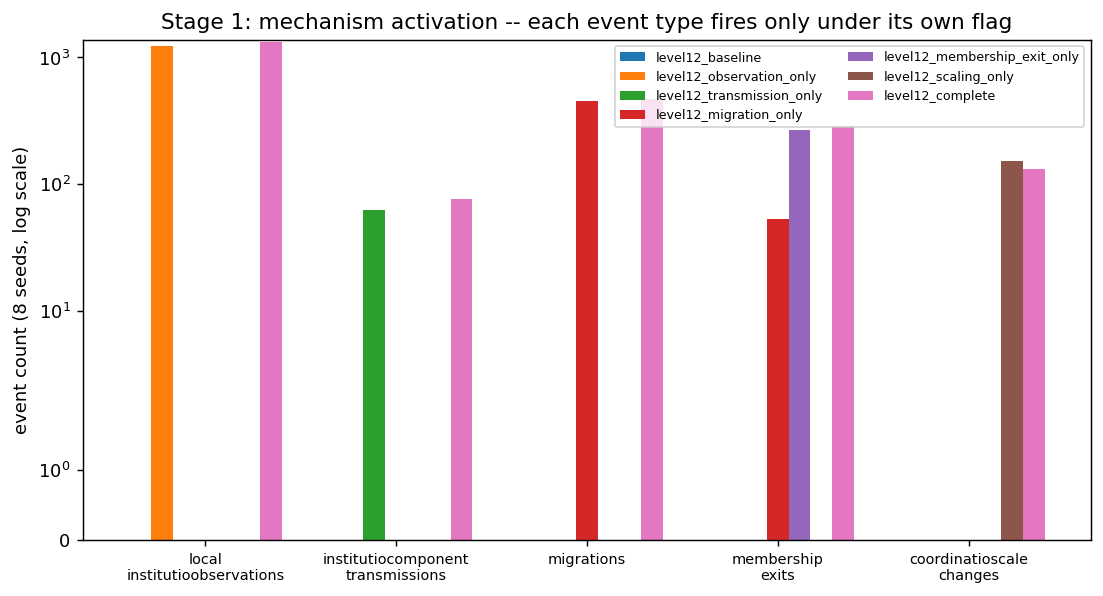
\includegraphics[width=0.75\textwidth]{figures/appendix/a_l12_stage1_activation.png}
\caption{Level 1.2 Stage 1: mechanism-activation totals across 7
conditions $\times$ 8 seeds (56 runs), confirming every new mechanism is
reachable and behaves as expected before any search stage runs.}
\end{figure}

\begin{figure}[htbp]
\centering
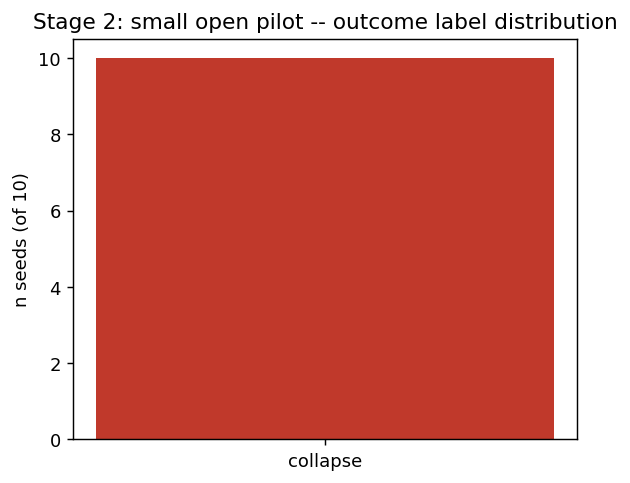
\includegraphics[width=0.7\textwidth]{figures/appendix/a_l12_stage2_outcome.png}
\caption{Level 1.2 Stage 2 small open pilot outcome distribution
($n$=10): 7 collapse, 3 fragmented, 0 viable.}
\end{figure}

\begin{figure}[htbp]
\centering
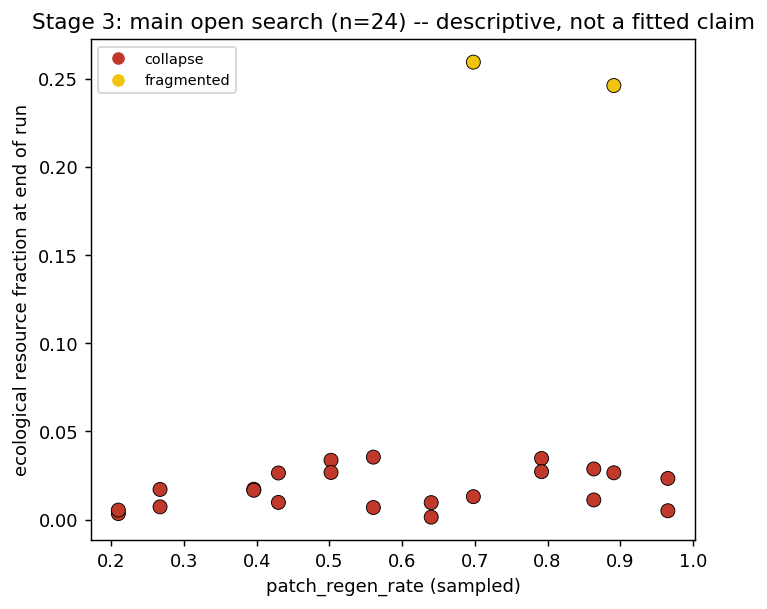
\includegraphics[width=0.75\textwidth]{figures/appendix/a_l12_stage3_regen_vs_eco.png}
\caption{Level 1.2 Stage 3: patch regeneration rate versus realized
ecological fraction across the 24-run main search --- the descriptive
association Section 13's regen-rate ablation later tested causally.}
\end{figure}

\begin{figure}[htbp]
\centering
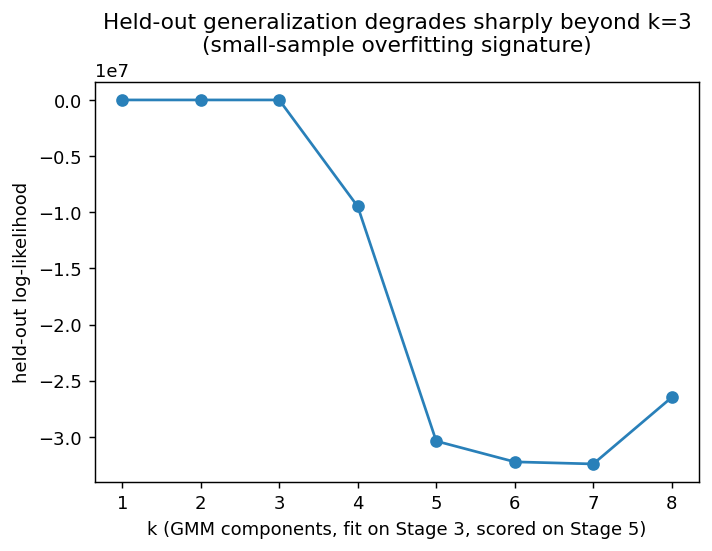
\includegraphics[width=0.7\textwidth]{figures/appendix/a_l12_stage5_heldout_ll.png}
\caption{Level 1.2 Stage 5: held-out log-likelihood by $k$, fit on Stage 3
and scored on Stage 5's fresh runs --- gradual degradation to $k$=3, then
catastrophic collapse at $k\geq4$, a small-sample Gaussian-mixture
overfitting signature.}
\end{figure}

\begin{figure}[htbp]
\centering
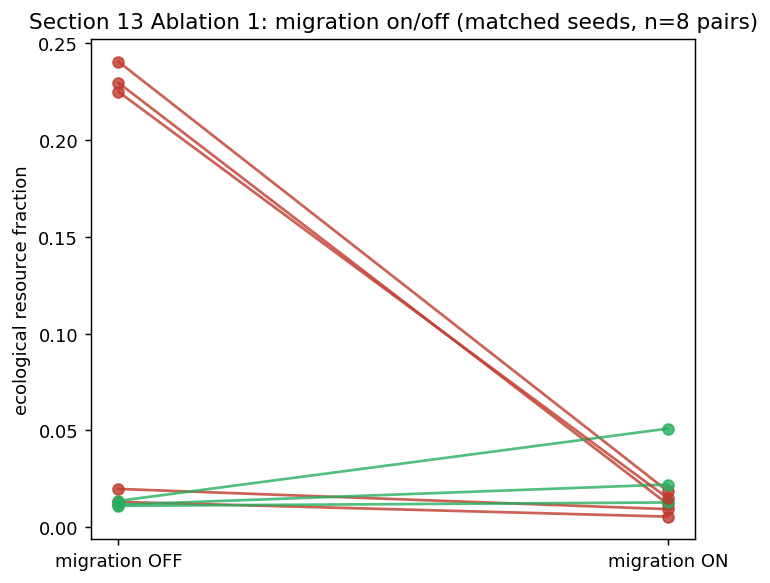
\includegraphics[width=0.85\textwidth]{figures/appendix/a_l12_stage13_migration_ablation.png}
\caption{Level 1.2 Section 13 matched-seed migration ablation
($n$=8 pairs): 5/8 pairs favor migration off on ecological fraction.}
\end{figure}

\begin{figure}[htbp]
\centering
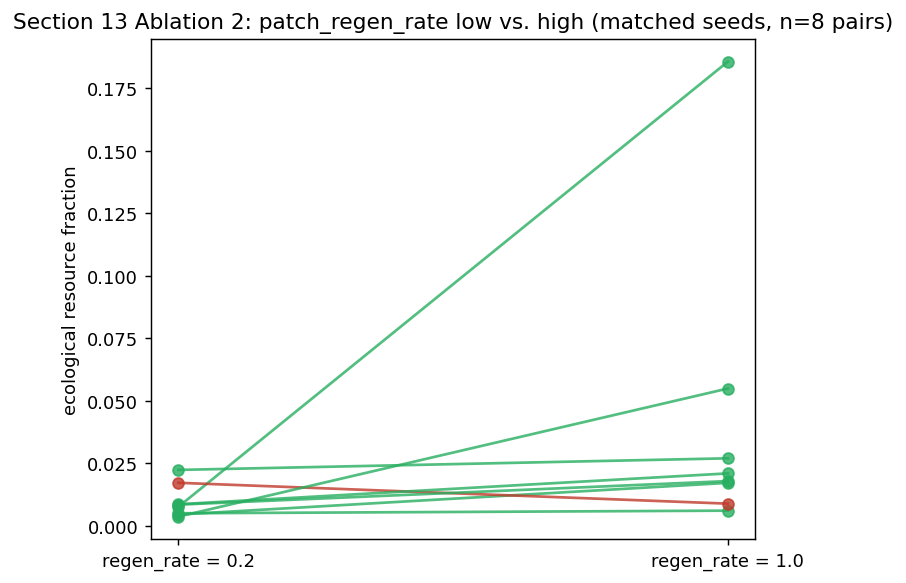
\includegraphics[width=0.85\textwidth]{figures/appendix/a_l12_stage13_regen_ablation.png}
\caption{Level 1.2 Section 13 matched-seed regeneration-rate ablation
($n$=8 pairs): 7/8 pairs favor the higher regeneration rate.}
\end{figure}

\begin{figure}[htbp]
\centering
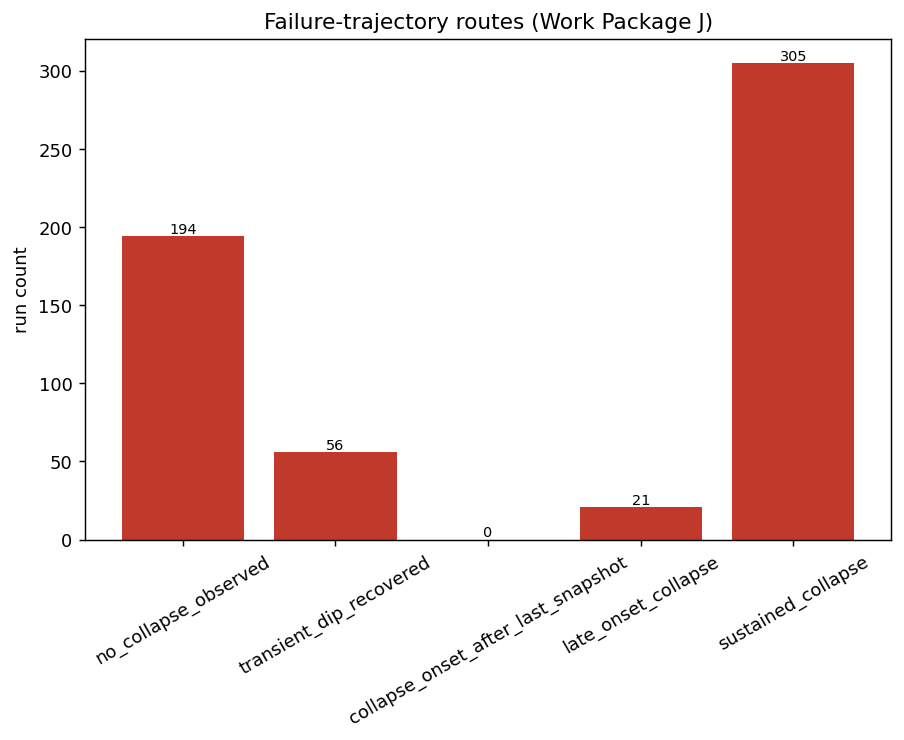
\includegraphics[width=0.75\textwidth]{figures/appendix/a_l12b_failure_trajectory.png}
\caption{Level 1.2b failure-trajectory classification, discovery pool
($n$=576): most collapse outcomes are \texttt{sustained\_collapse}, not a
last-instant artifact.}
\end{figure}

\begin{figure}[htbp]
\centering
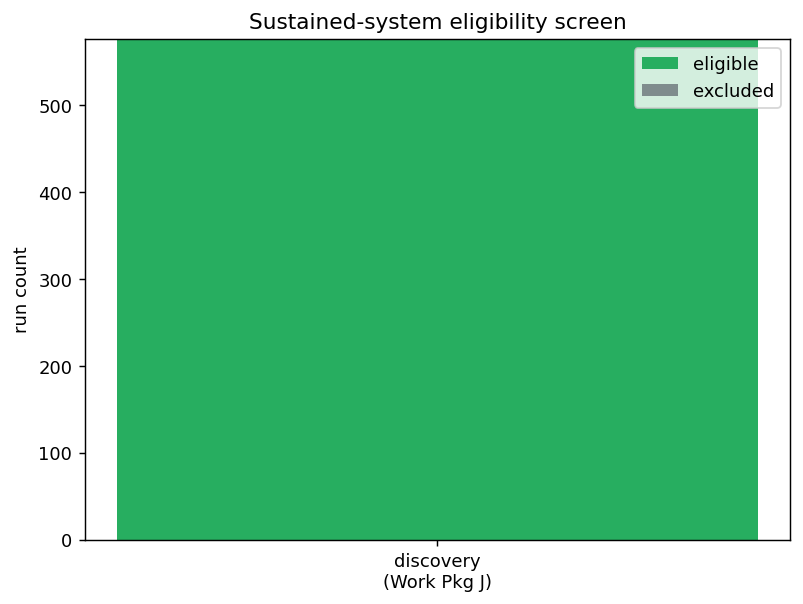
\includegraphics[width=0.7\textwidth]{figures/appendix/a_l12b_sustained_eligibility.png}
\caption{Level 1.2b sustained-system data-sufficiency screen: all 576
discovery runs eligible, 0 excluded, comfortably above both the preferred
(60) and hard-minimum (40) gates.}
\end{figure}

\begin{figure}[htbp]
\centering
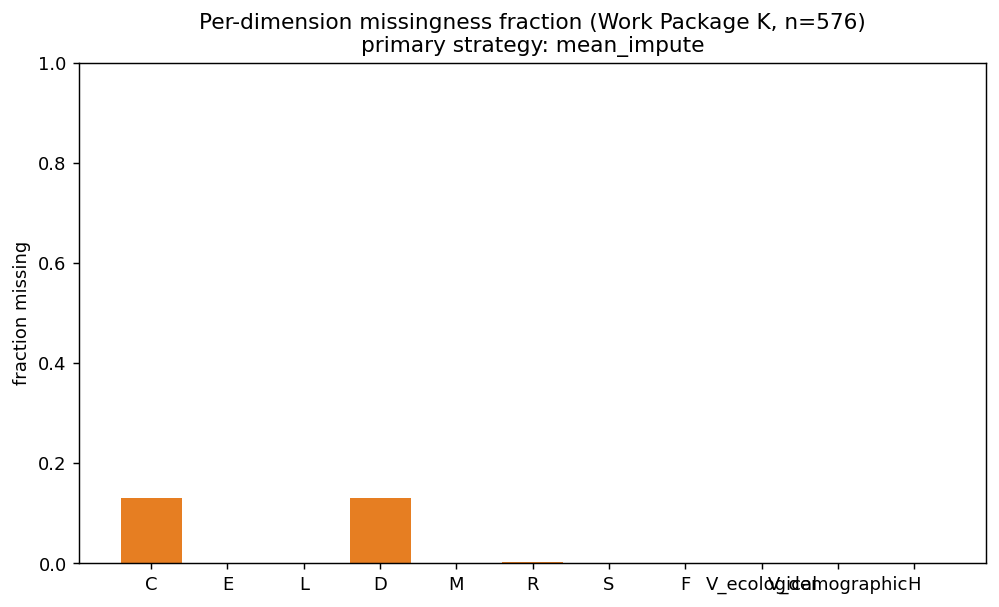
\includegraphics[width=0.7\textwidth]{figures/appendix/a_l12b_missingness.png}
\caption{Level 1.2b phenotype-feature missingness by dimension, discovery
pool ($n$=576).}
\end{figure}

\begin{figure}[htbp]
\centering
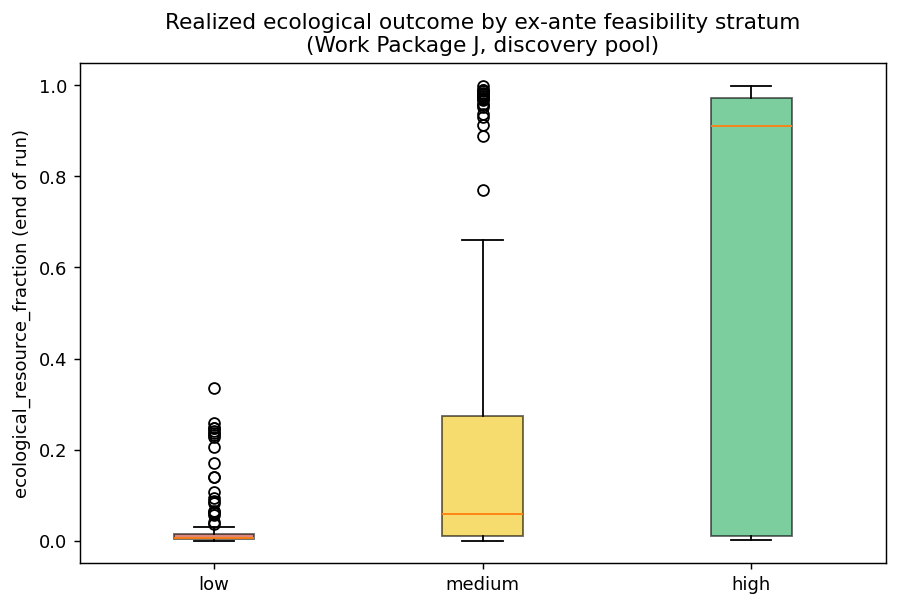
\includegraphics[width=0.85\textwidth]{figures/appendix/a_l12b_feature_by_stratum.png}
\caption{Level 1.2b phenotype-feature distributions by ecological stratum
(low/medium/high expected-pressure ratio).}
\end{figure}

\begin{figure}[htbp]
\centering
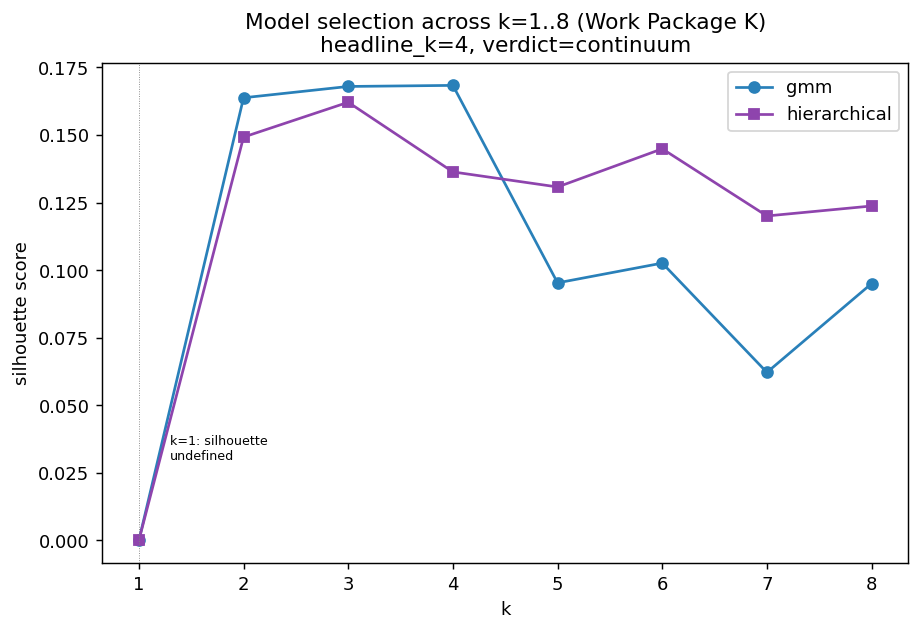
\includegraphics[width=0.8\textwidth]{figures/appendix/a_l12b_model_selection.png}
\caption{Level 1.2b model-selection metrics (silhouette,
Calinski--Harabasz, Davies--Bouldin) by $k$, discovery pool.}
\end{figure}

\begin{figure}[htbp]
\centering
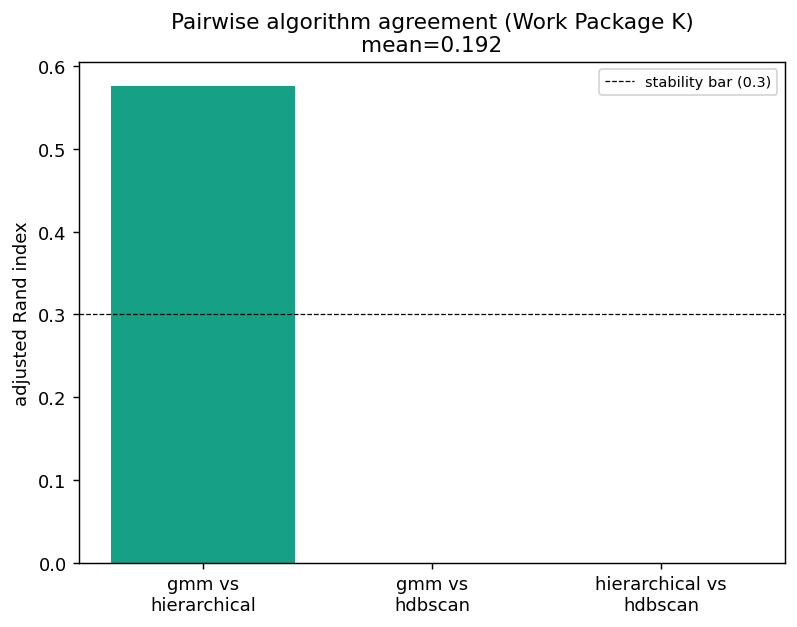
\includegraphics[width=0.75\textwidth]{figures/appendix/a_l12b_algorithm_agreement.png}
\caption{Level 1.2b pairwise algorithm-agreement (adjusted Rand index)
between Gaussian mixture, hierarchical, and \texttt{HDBSCAN} fits.}
\end{figure}

\begin{figure}[htbp]
\centering
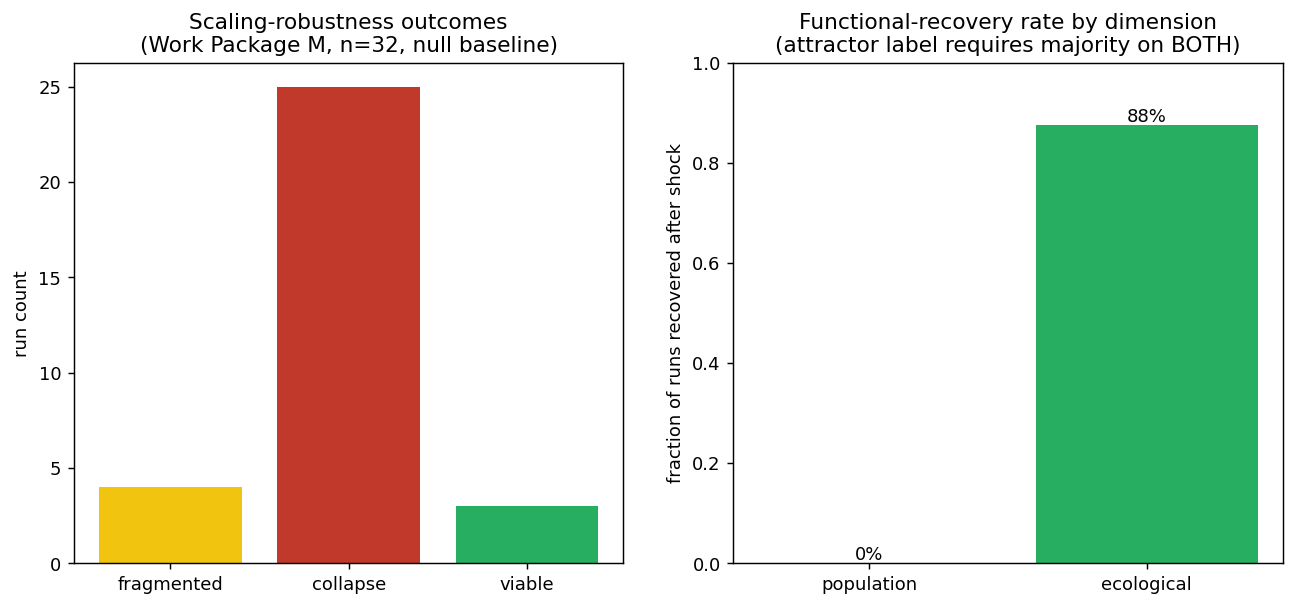
\includegraphics[width=0.85\textwidth]{figures/appendix/a_l12b_scaling_robustness.png}
\caption{Level 1.2b Work Package M scaling-robustness grid: outcome and
recovery detail across population $\times$ patch-count $\times$
modularity conditions ($n$=32).}
\end{figure}

\begin{figure}[htbp]
\centering
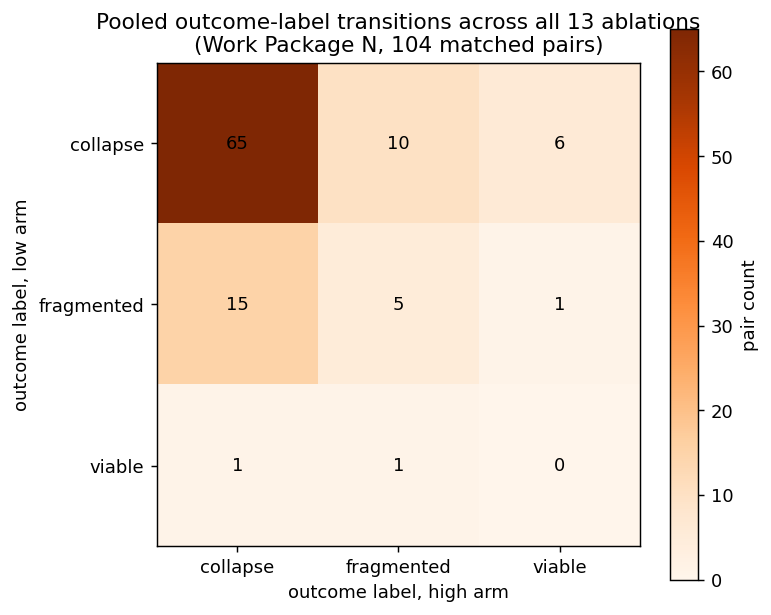
\includegraphics[width=0.75\textwidth]{figures/appendix/a_l12b_outcome_transition_matrix.png}
\caption{Level 1.2b outcome-label transition matrix, discovery versus
confirmation pools.}
\end{figure}

\begin{figure}[htbp]
\centering
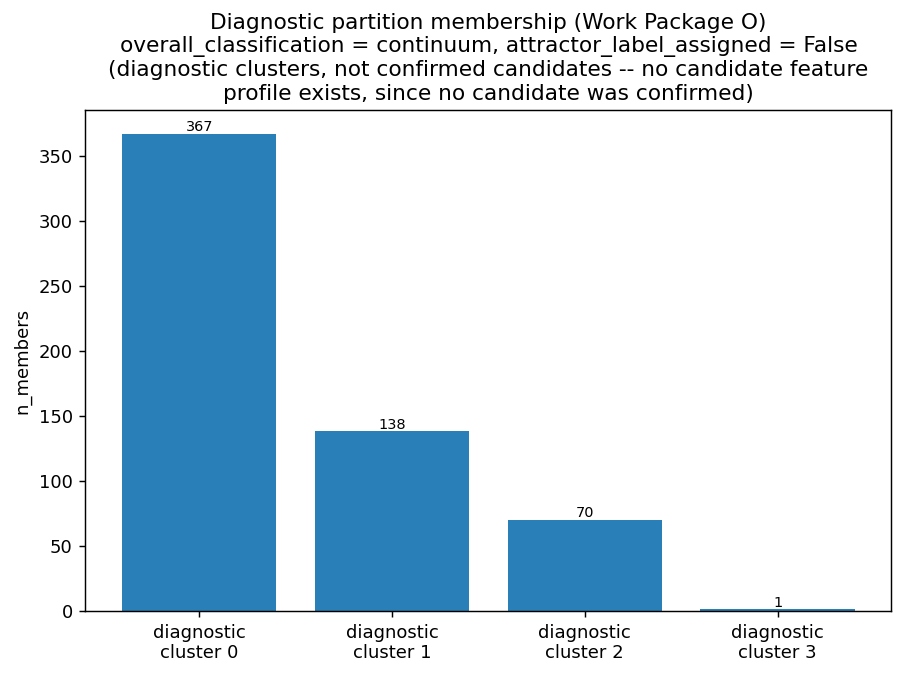
\includegraphics[width=0.75\textwidth]{figures/appendix/a_l12b_recurrence_classification.png}
\caption{Level 1.2b Work Package O overall recurrence classification
summary: \texttt{continuum}, \texttt{attractor\_label\_assigned=False}.}
\end{figure}

\begin{figure}[htbp]
\centering
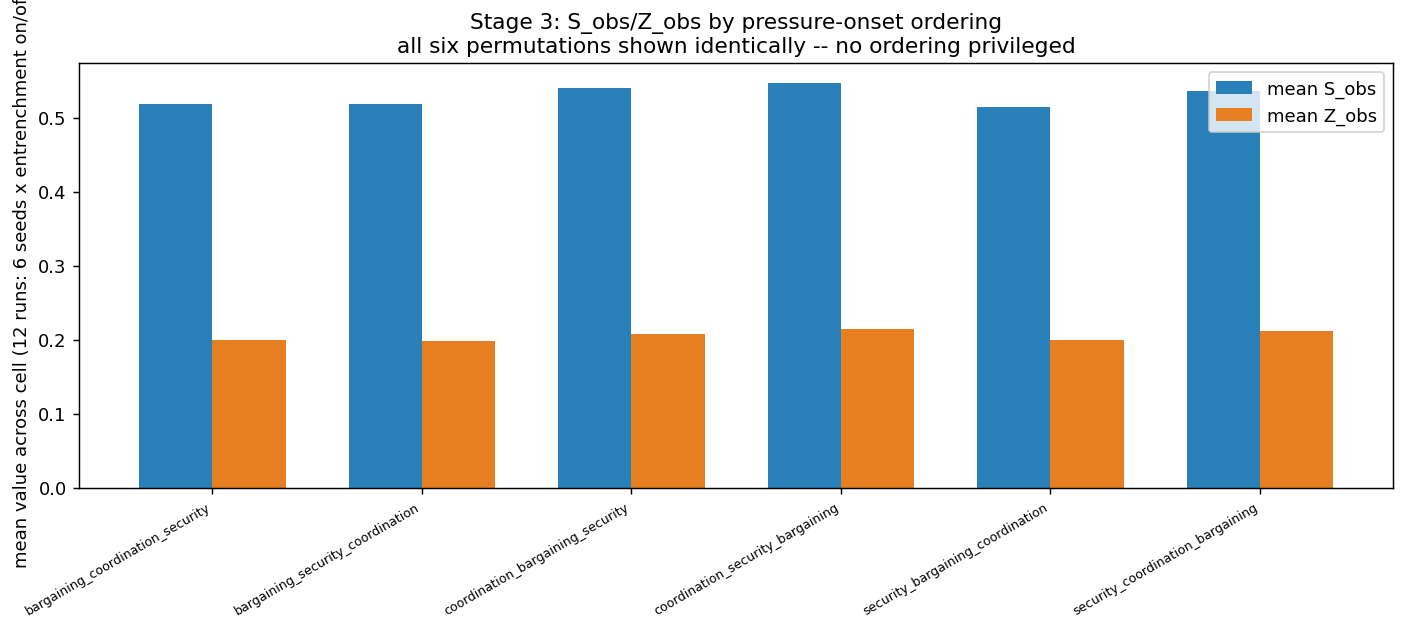
\includegraphics[width=0.85\textwidth]{figures/appendix/a_l13_stage3_by_ordering.png}
\caption{Level 1.3 Stage 3: mean $S_{\text{obs}}$/$Z_{\text{obs}}$ by
pressure-onset ordering (72-run matched factorial, six orderings),
descriptive precursor to Level 1.3b's own purpose-designed Stage 3
factorial (\cref{fig:l13b-ordering}).}
\end{figure}

\begin{figure}[htbp]
\centering
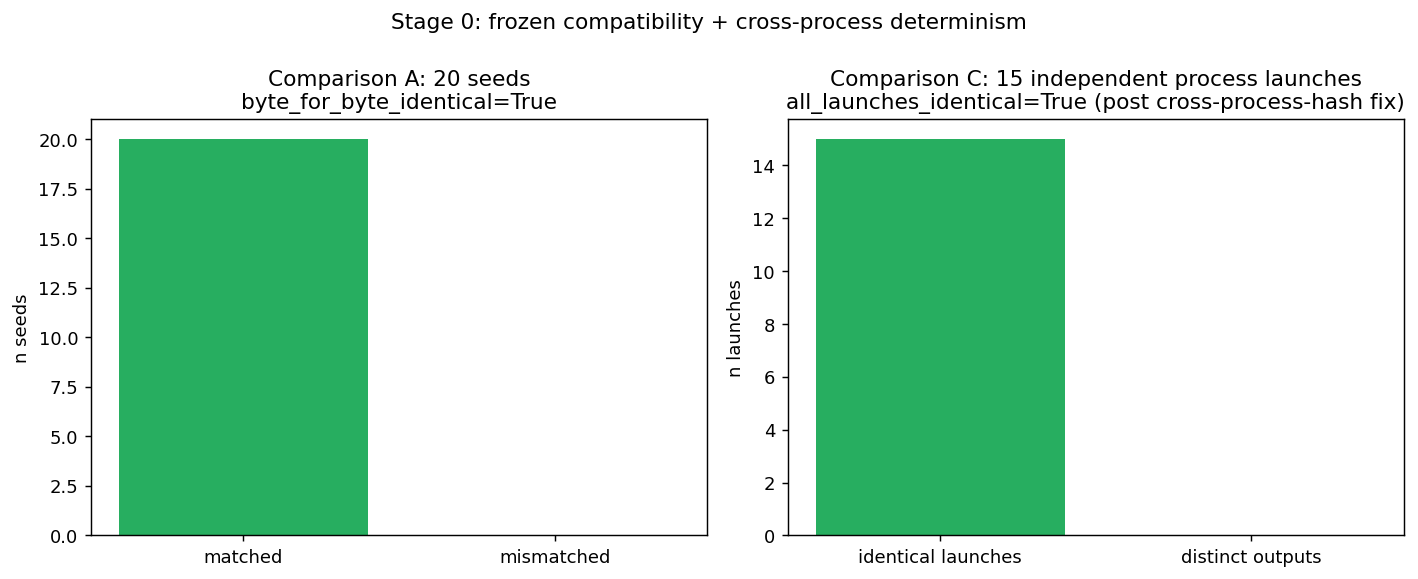
\includegraphics[width=0.75\textwidth]{figures/appendix/a_l13b_cross_process_repro.png}
\caption{Level 1.3b Stage 0: cross-process determinism comparison. 15
distinct outputs pre-fix (frozenset-hash non-determinism), 1 identical
output post-fix, across 15 separate process launches of the identical
seed and configuration.}
\end{figure}

\begin{figure}[htbp]
\centering
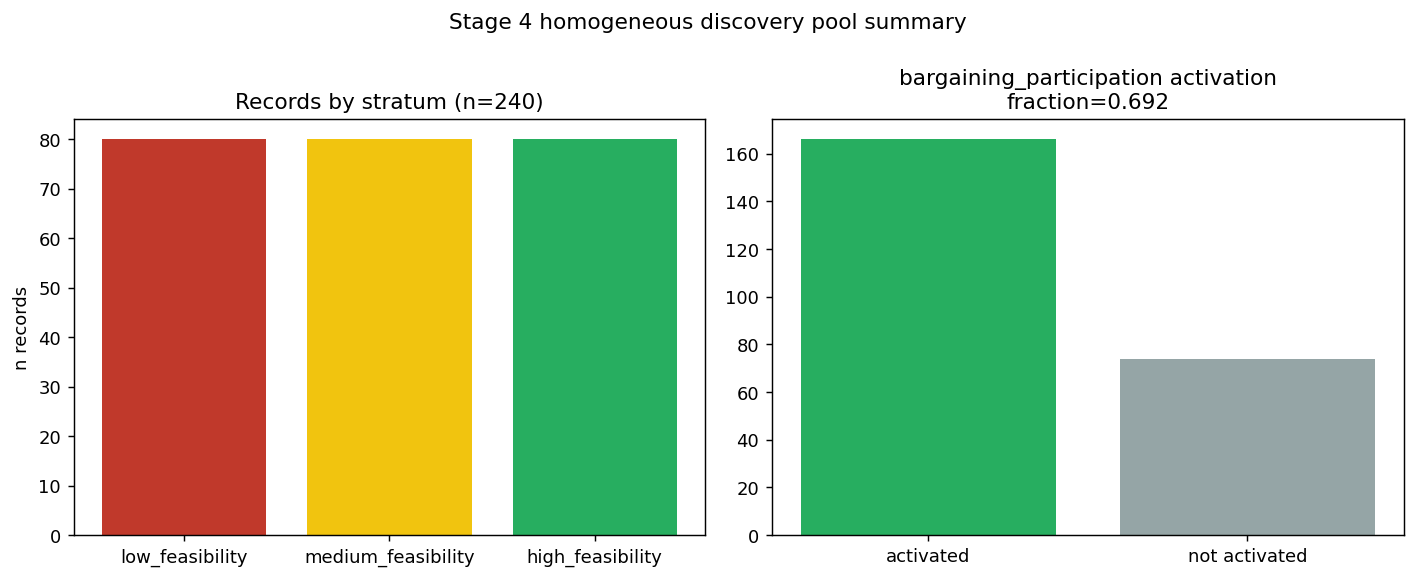
\includegraphics[width=0.8\textwidth]{figures/appendix/a_l13b_stage4_pool_summary.png}
\caption{Level 1.3b Stage 4: 240-run homogeneous discovery pool summary
(the purpose-designed successor to Level 1.3's own pooled 216-run
sample).}
\end{figure}

\begin{figure}[htbp]
\centering
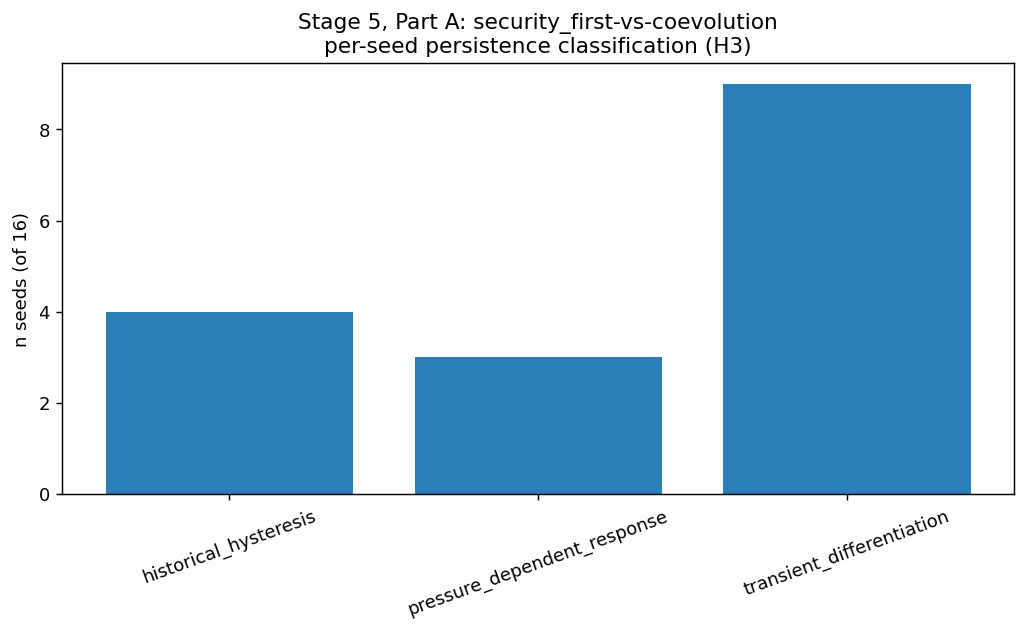
\includegraphics[width=0.8\textwidth]{figures/appendix/a_l13b_persistence_classification.png}
\caption{Level 1.3b Stage 5 Part A: per-seed persistence classification
(16 matched seeds, \texttt{security\_first} vs.\ \texttt{coevolution}) ---
9/16 \texttt{transient\_differentiation}, 4/16 \texttt{historical\_%
hysteresis}, 3/16 \texttt{pressure\_dependent\_response}, 0/16
\texttt{entrenched\_path\_dependence}.}
\end{figure}

\begin{figure}[htbp]
\centering
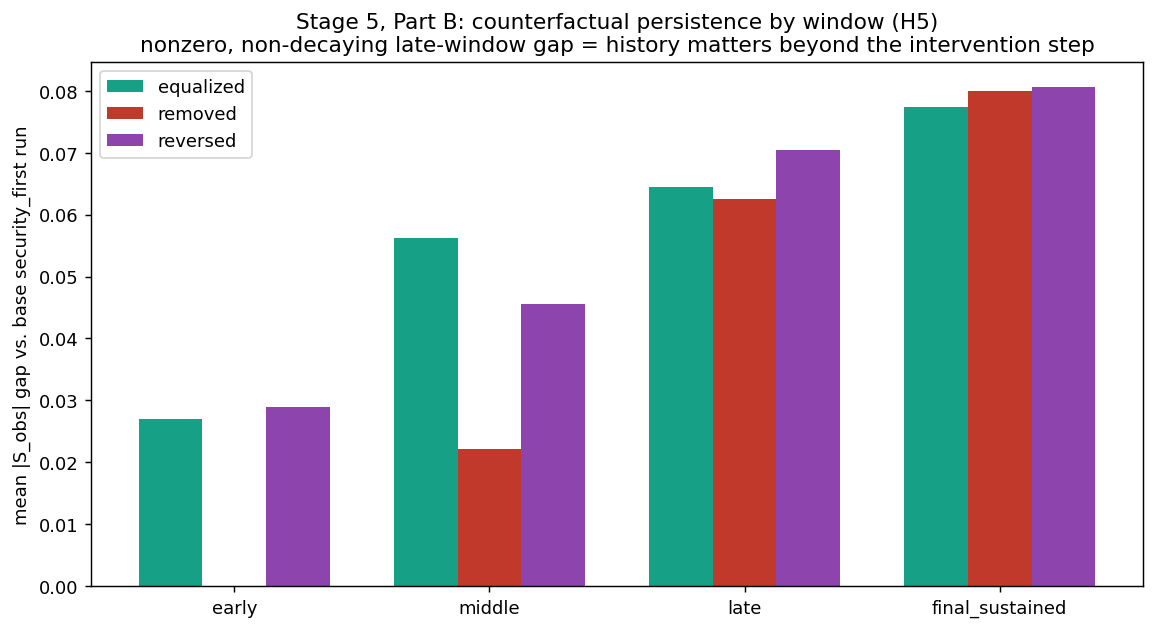
\includegraphics[width=0.8\textwidth]{figures/appendix/a_l13b_counterfactual_persistence.png}
\caption{Level 1.3b Stage 5 Part B: counterfactual-persistence gap by
window for the \texttt{removed}/\texttt{reversed}/\texttt{equalized}
pressure-history transforms versus the base \texttt{security\_first} run.}
\end{figure}

\begin{figure}[htbp]
\centering
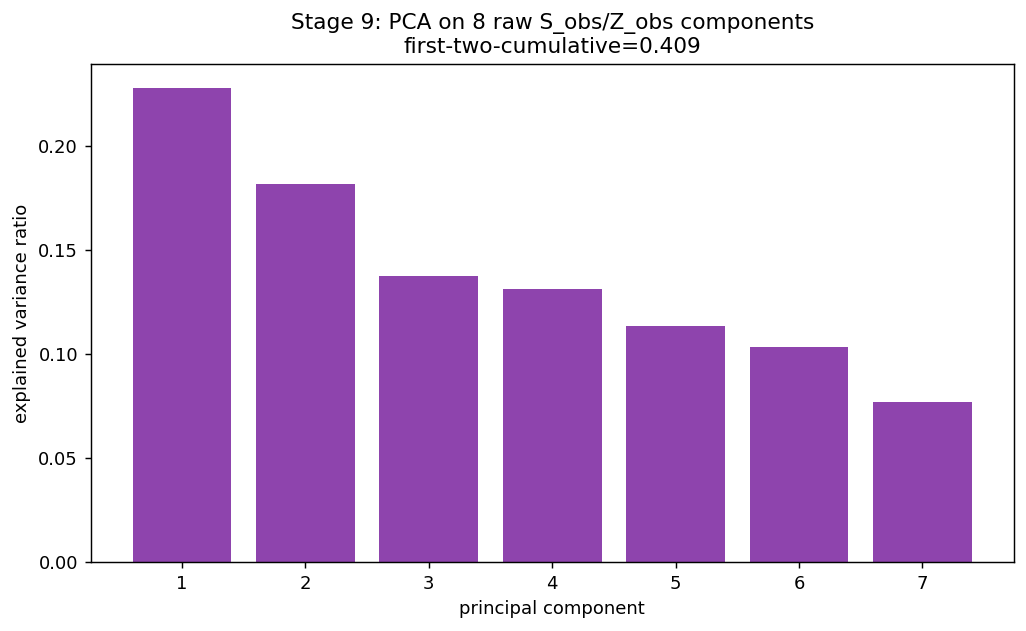
\includegraphics[width=0.75\textwidth]{figures/appendix/a_l13b_factor_structure.png}
\caption{Level 1.3b Stage 9: data-driven factor-structure analysis. PC1
(22.8\% of variance) is loaded by both legitimacy channels together
(0.654 performance, 0.674 procedural) rather than splitting cleanly along
an $S$-axis/$Z$-axis line; scree flat, top-two cumulative 40.9\%.}
\end{figure}

\begin{figure}[htbp]
\centering
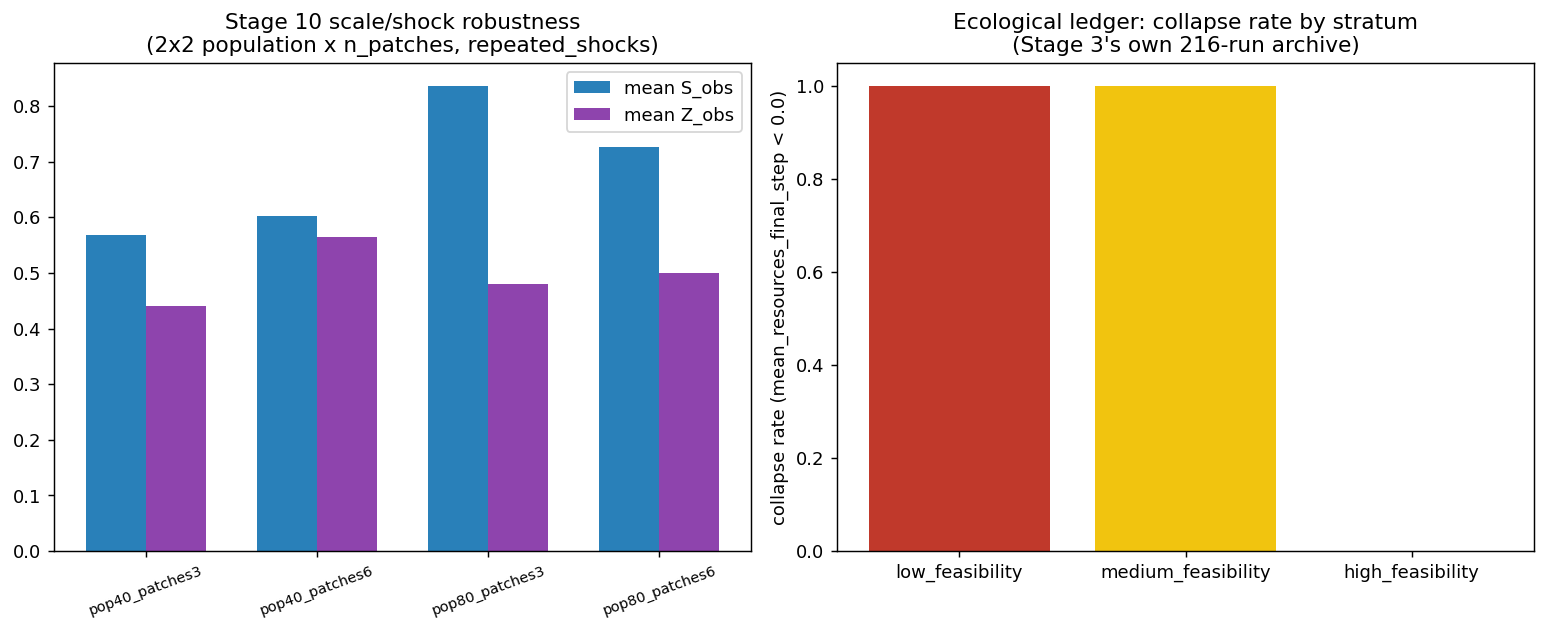
\includegraphics[width=0.75\textwidth]{figures/appendix/a_l13b_scale_and_ledger.png}
\caption{Level 1.3b Stage 10: ecological-control scale-shock check (24
runs) under the historically extended substrate.}
\end{figure}

\begin{figure}[htbp]
\centering
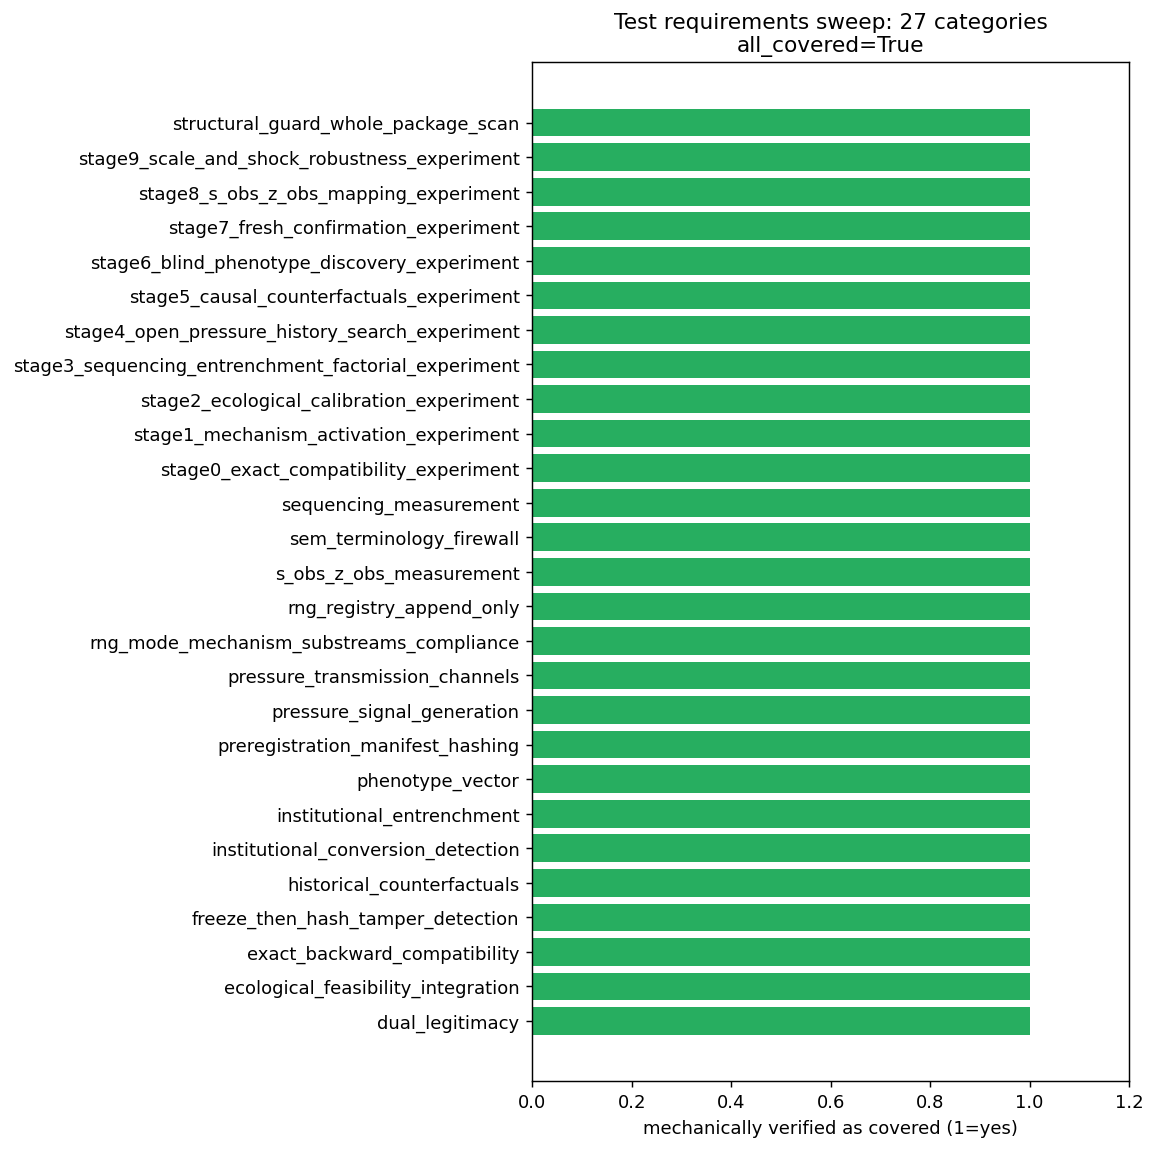
\includegraphics[width=0.9\textwidth]{figures/appendix/a_l13_test_requirements_coverage.png}
\caption{Level 1.3 test-requirements coverage matrix.}
\end{figure}

\begin{figure}[htbp]
\centering
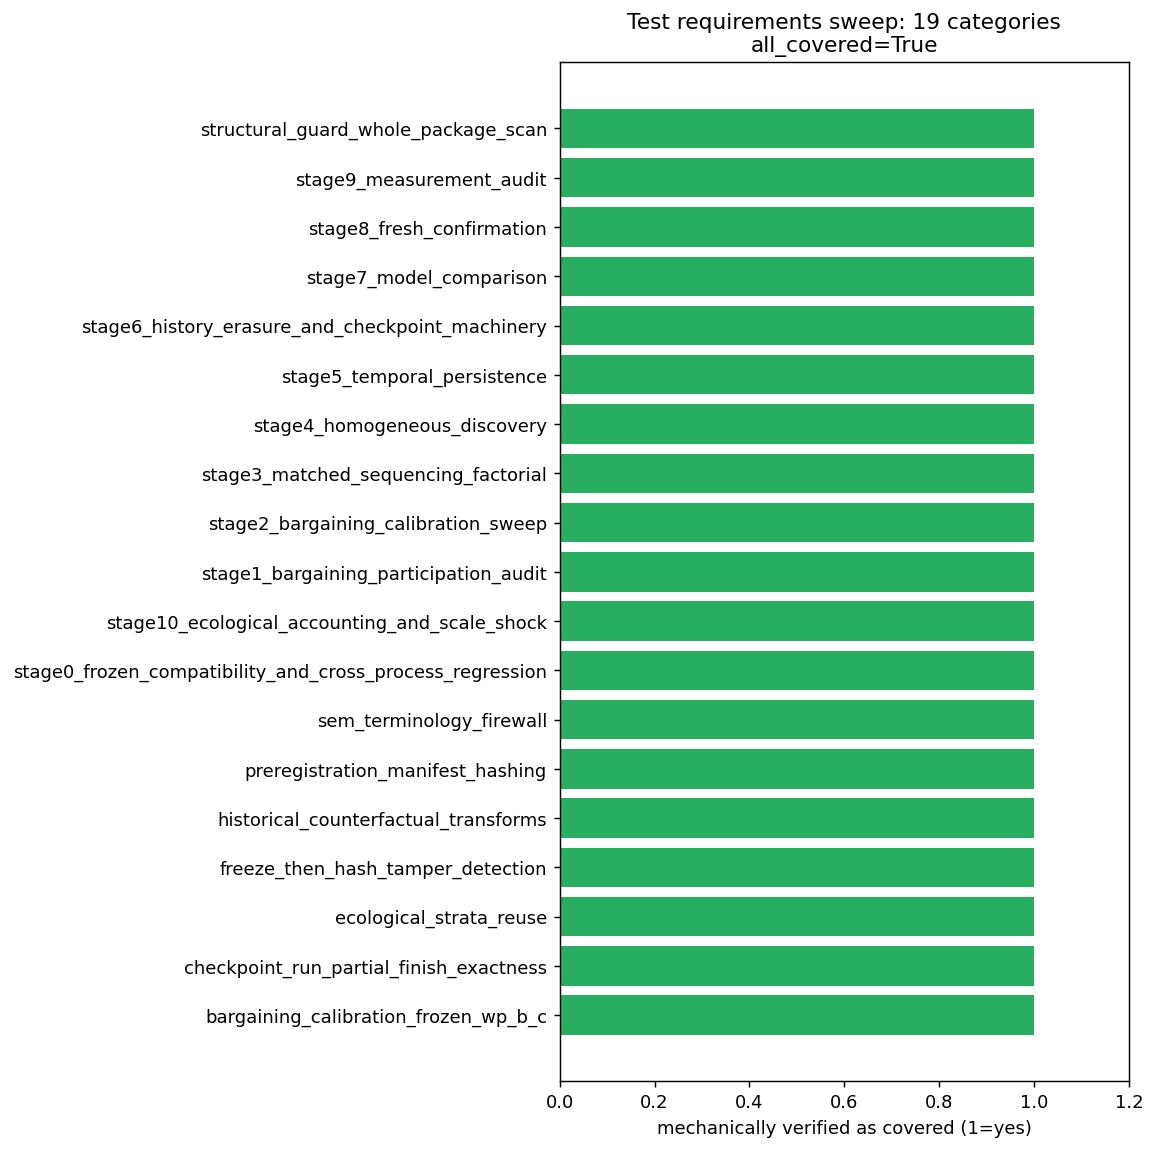
\includegraphics[width=0.9\textwidth]{figures/appendix/a_l13b_test_requirements_coverage.png}
\caption{Level 1.3b test-requirements coverage matrix (19 categories,
including two negative controls proving the checker can actually fail).}
\end{figure}


\end{document}
